% file: main.tex


% TODO

% Add clarification on semantics of define-fun for case of n=0
% Add more entries to Index


%\documentclass[10pt,twoside]{report}
\documentclass[11pt]{report}
\usepackage[Sonny]{fncychap}
% Sonny, Lenny, Glenn, Conny, Rejne, Bjarne, PetersLenny, Bjornstrup
\ChTitleVar{\huge\sf}
\ChNameVar{\large\sf}
\ChNumVar{\Huge}
\ChRuleWidth{1pt}

\usepackage[T1]{fontenc}
%\usepackage{lxfonts}
%\usepackage[math]{kurier}
%\usepackage[sfmath]{kpfonts}
%\usepackage{kpfonts}
%\usepackage[math]{iwona}
%\usepackage{arev}
\usepackage[sc]{mathpazo}
\linespread{1.04}         % Palladio needs more leading (space between lines)

\usepackage{multicol}

% This gives an acceptable placement of the bounding box on the page:
%\usepackage[a4paper]{geometry}
\usepackage{geometry}
\geometry{
textwidth=160mm,
top=35mm,
bottom=25mm,
%textheight=26cm,
nofoot,
headsep=8mm,
headheight=14pt
}

\newcommand{\headerfont}{\textnormal}

%\usepackage{draftwatermark}
%\SetWatermarkScale{1.1}
%\SetWatermarkLightness{0.97}

\usepackage{fancyhdr}
\pagestyle{fancy}
%\renewcommand{\subsectionmark}[1]{\markright{\thesection\quad #1}}
\lhead[\fancyplain{}{\thepage}]{\fancyplain{}{\headerfont{\rightmark}}}
%  i.e. empty on ``plain'' pages, \thepage on even, \rightmark on odd pages
\chead{}
\rhead[\fancyplain{}{\headerfont{\nouppercase{\leftmark}}}]{\fancyplain{}{\thepage}}
%  i.e. empty on ``plain'' pages, \leftmark on even, \thepage on odd pages
\lfoot{}
\cfoot{} % page number
\rfoot{}

\usepackage{verbatim}
\usepackage{amsmath,amssymb,amsthm}
\usepackage{xspace}
\usepackage{makeidx}
\usepackage{tocbibind}
\usepackage[usenames,dvipsnames,svgnames,table]{xcolor}


\usepackage{pgf}
\usepackage{tikz}
%\usepackage[active,tightpage]{preview}
%%\PreviewEnvironment{tikzpicture}
%%\setlength\PreviewBorder{5pt}%
\usepackage[utf8]{inputenc}
\usetikzlibrary{arrows,automata}
\usetikzlibrary{positioning}
\tikzset{
    state/.style={
           rectangle,
           rounded corners,
           draw=black, very thick,
           minimum height=2em,
           inner sep=2pt,
           text centered,
           },
}


\usepackage{listings}
\lstset{%
%frameround=tttt,
frame=shadowbox, 
basicstyle=\small\ttfamily\color{NavyBlue},
%frame=trBL,
%color=\color{blue},
rulesepcolor=\color{black},
showstringspaces=false,
xleftmargin=2em,
aboveskip=\bigskipamount,
belowskip=\bigskipamount}
%language=Lisp}
%\lstloadlanguages{Lisp}


\usepackage{hyperref}
\hypersetup{
 colorlinks=true,
 linkcolor=Grey, %DarkSlateBlue
 citecolor=Grey,
 urlcolor=Grey,
 pdftitle=The SMT-LIB Standard,
 pdfauthor=Clark Barrett; Pascal Fontaine; Aaron Stump; Cesare Tinelli
 pdfkeywords=SMT-LIB standard
}
\usepackage{endnotes}
%\documentclass{article}
%\usepackage{hyperref}
%\usepackage{endnotes}
\makeatletter
\newif\ifenotelinks
\newcounter{Hendnote}
% Redefining portions of endnotes-package:
\let\savedhref\href
\let\savedurl\url
\def\endnotemark{%
\@ifnextchar[\@xendnotemark{%
\stepcounter{endnote}%
\protected@xdef\@theenmark{\theendnote}%
\protected@xdef\@theenvalue{\number\c@endnote}%
\@endnotemark
}%
}%
\def\@xendnotemark[#1]{%
\begingroup\c@endnote#1\relax
\unrestored@protected@xdef\@theenmark{\theendnote}%
\unrestored@protected@xdef\@theenvalue{\number\c@endnote}%
\endgroup
\@endnotemark
}%
\def\endnotetext{%
\@ifnextchar[\@xendnotenext{%
\protected@xdef\@theenmark{\theendnote}%
\protected@xdef\@theenvalue{\number\c@endnote}%
\@endnotetext
}%
}%
\def\@xendnotenext[#1]{%
\begingroup
\c@endnote=#1\relax
\unrestored@protected@xdef\@theenmark{\theendnote}%
\unrestored@protected@xdef\@theenvalue{\number\c@endnote}%
\endgroup
\@endnotetext
}%
\def\endnote{%
\@ifnextchar[\@xendnote{%
\stepcounter{endnote}%
\protected@xdef\@theenmark{\theendnote}%
\protected@xdef\@theenvalue{\number\c@endnote}%
%ct \@endnotemark\@endnotetext
$^($\@endnotemark$^)$\@endnotetext
}%
}%
\def\@xendnote[#1]{%
\begingroup
\c@endnote=#1\relax
\unrestored@protected@xdef\@theenmark{\theendnote}%
\unrestored@protected@xdef\@theenvalue{\number\c@endnote}%
\show\@theenvalue
\endgroup
\@endnotemark\@endnotetext
}%
\def\@endnotemark{%
\leavevmode
\ifhmode
\edef\@x@sf{\the\spacefactor}\nobreak
\fi
\ifenotelinks
\expandafter\@firstofone
\else
\expandafter\@gobble
\fi
{%
\Hy@raisedlink{%
\hyper@@anchor{Hendnotepage.\@theenvalue}{\empty}%
}%
}%
\hyper@linkstart{link}{Hendnote.\@theenvalue}%
\makeenmark
\hyper@linkend
\ifhmode
\spacefactor\@x@sf
\fi
\relax
}%
\long\def\@endnotetext#1{%
\if@enotesopen
\else
\@openenotes
\fi
\immediate\write\@enotes{%
\@doanenote{\@theenmark}{\@theenvalue}%
}%
\begingroup
\def\next{#1}%
\newlinechar='40
\immediate\write\@enotes{\meaning\next}%
\endgroup
\immediate\write\@enotes{%
\@endanenote
}%
}%
\def\theendnotes{%
\immediate\closeout\@enotes
\global\@enotesopenfalse
\begingroup
\makeatletter
\edef\@tempa{`\string>}%
\ifnum\catcode\@tempa=12
\let\@ResetGT\relax
\else
\edef\@ResetGT{\noexpand\catcode\@tempa=\the\catcode\@tempa}%
\@makeother\>%
\fi
\def\@doanenote##1##2##3>{%
\def\@theenmark{##1}%
\def\@theenvalue{##2}%
\par
\smallskip %<-small vertical gap between endnotes
\begingroup
\def\href{\expandafter\savedhref}%
\def\url{\expandafter\savedurl}%
\@ResetGT
\edef\@currentlabel{\csname p@endnote\endcsname\@theenmark}%
\enoteformat
}%
\def\@endanenote{%
\par\endgroup
}%
% Redefine, how numbers are formatted in the endnotes-section:
\renewcommand*\@makeenmark{%
\hbox{\normalfont\@theenmark~}%
}%
% header of endnotes-section
%ct \enoteheading
% font-size of endnotes
\enotesize
\input{\jobname.ent}%
\endgroup
}%
\def\enoteformat{%
\rightskip\z@
\leftskip1.8em
\parindent\z@
\leavevmode\llap{%
\setcounter{Hendnote}{\@theenvalue}%
\addtocounter{Hendnote}{-1}%
\refstepcounter{Hendnote}%
\ifenotelinks
\expandafter\@secondoftwo
\else
\expandafter\@firstoftwo
\fi
{\@firstofone}%
{\hyperlink{Hendnotepage.\@theenvalue}}%
{\makeenmark}%
}%
}%
% stop redefining portions of endnotes-package:
\makeatother
%
%% Toggle switch in order to turn on/off back-links in the
%% endnote-section:
%\enotelinkstrue
%%\enotelinksfalse
%\begin{document}
%\addtocounter{section}{9}
%\section{test}

%A footnote works fine.%
%\footnote{Use \href{http://docs.python.org}{Python}.}

%A broken footnote also works fine.\footnotemark[4]%
%\footnotetext[4]{%
%Where is \href{http://docs.python.org}{Python}?
%Here: \url{http://docs.python.org}
%}

%An endnote does work now.%
%\endnote{%
%\label{enoteA}%
%Why not using \href{http://docs.python.org}{Python}?
%Here you find it: \url{http://docs.python.org}
%multi line text multi line text multi line text
%multi line text multi line text multi line text
%multi line text multi line text multi line text
%multi line text multi line text multi line text
%}

%You can also break it up.\endnotemark[4]\label{enoteB}%
%\endnotetext[4]{%
%\label{enoteC}%
%Where is \href{http://docs.python.org}{Python}?
%Here: \url{http://docs.python.org}
%multi line text multi line text multi line text
%multi line text multi line text multi line text
%multi line text multi line text multi line text
%multi line text multi line text multi line text
%}

%You can also break it up.\endnotemark[10]\label{enoteD}%
%\endnotetext[10]{%
%\label{enoteE}%
%Where is \href{http://docs.python.org}{Python}?
%Here: \url{http://docs.python.org}
%multi line text multi line text multi line text
%multi line text multi line text multi line text
%multi line text multi line text multi line text
%multi line text multi line text multi line text
%}

%You can also break it up.\endnotemark[100]\label{enoteF}%
%\endnotetext[100]{%
%\label{enoteG}%
%Where is \href{http://docs.python.org}{Python}?
%Here: \url{http://docs.python.org}
%multi line text multi line text multi line text
%multi line text multi line text multi line text
%multi line text multi line text multi line text
%multi line text multi line text multi line text
%}

%Continue in text\label{enoteH}.

%Reference in endnote: \ref{enoteA}.

%Reference in text after endnote-mark: \ref{enoteB}.

%Reference in endnote-text: \ref{enoteC}.

%Reference in text after endnote-text: \ref{enoteD}.

%Reference in endnote-text: \ref{enoteE}.

%Reference in text after endnote-text: \ref{enoteF}.

%Reference in endnote-text: \ref{enoteG}.

%Reference in Text: \ref{enoteH}
%\newpage
%\theendnotes

%\end{document}

% Toggle switch in order to turn on/off back-links in the endnote-section:
\enotelinkstrue
%\enotelinksfalse

\makeindex

%!TEX root = main.tex

% macros.tex

\newcommand{\thisversion}{Version 2.6\xspace}

\newcommand{\rem}[2]{\textsf{[#1: #2]}}
\newcommand{\cbrem}[1]{\rem{CB}{#1}}
\newcommand{\asrem}[1]{\rem{AS}{#1}}
\newcommand{\ctrem}[1]{\rem{CT}{#1}}
%\newcommand{\ctrem}[1]{\ignorespaces}

\newcommand{\new}[1]{{\color{FireBrick} #1}}
\newenvironment{newver}{\color{FireBrick}}{}
%\newcommand{\new}[1]{#1}
%\newenvironment{newver}{}{}
\newcommand{\adt}{\marginpar{[adts]}}

\newcommand{\Section}[1]{
 \newpage
 \section{#1}}

\theoremstyle{definition} 
\newtheorem{theorem}{Theorem}
\newtheorem{definition}[theorem]{Definition}
\newtheorem{constraint}{Constraint}
\newtheorem{remark}{Remark}
%\newtheorem{example}{Example}


\newenvironment{com}
{\rule{1ex}{1ex}%
\hspace{\stretch{1}}} 
{\hspace{\stretch{1}}%
\rule{1ex}{1ex}}

%\newcommand{\define}[1]{{\textcolor{MediumBlue}{\textsl{#1}}}}
\newcommand{\define}[1]{{\textcolor{Maroon}{\textsl{#1}}}}

\newcommand{\mode}[1]{\textsf{#1}}

\newcommand{\note}[1]{$^{\langle\ref{#1}\rangle}$}

\newcommand{\notetext}[2]{
\begin{designNote} \label{#1}
#2
\end{designNote}}


%\newcommand{\extra}[1]{{\small \sf #1}}
\newcommand{\extra}[1]{}

\newcommand{\dec}[1]{{#1}$_\mathrm{dec}$}
\newcommand{\hex}[1]{{#1}$_\mathrm{hex}$}

\newcommand{\str}[1]{\mathbf{#1}}
\newcommand{\inter}[1]{\mathcal{#1}}
\newcommand{\uni}[1]{\mathrm{#1}}
\newcommand{\eqs}{\approx}
\newcommand{\true}{\akey{true}}
\newcommand{\false}{\akey{false}}
\newcommand{\sorts}[1]{#1^\mathrm{S}}
\newcommand{\funs}[1]{#1^\mathrm{F}}
\newcommand{\cons}[1]{#1^\mathrm{C}}
\newcommand{\sels}[1]{#1^\mathrm{G}}
\newcommand{\tests}[1]{#1^\mathrm{T}}
\newcommand{\sortt}[1]{\mathit{Sort}(#1)}
%\newcommand{\subsorts}[1]{#1^{<:}}
\newcommand{\abset}[1]{\mathcal{#1}}
\newcommand{\so}{\abset{S}}
\newcommand{\fu}{\abset{F}}
\newcommand{\va}{\abset{X}}
\newcommand{\val}{\abset{V}}
\newcommand{\bo}{\abset{B}}
\newcommand{\at}{\abset{A}}
\newcommand{\ra}{\abset{R}}
\newcommand{\st}{\abset{W}}
\newcommand{\na}{\abset{N}}
\newcommand{\sop}{\abset{U}}
\newcommand{\la}{\abset{L}}
\newcommand{\te}{\abset{TN}}
\newcommand{\lo}{\abset{L}}
\newcommand{\pf}{\abset{P}}


\newcommand{\T}{\mathcal{T}}

\newcommand{\ar}{\mathrm{ar}}

\newlength{\brackt}
\settowidth{\brackt}{$[$}
\newcommand{\db}[1]{[\hspace{-.5\brackt}[{#1}]\hspace{-.5\brackt}]}
\newcommand{\mea}[2]{\db{#2}^{#1}}


\newcommand{\vars}[1]{\mathcal{V}\mathit{ar}(#1)}
%\newcommand{\fol}{$\mathit{FOL}^=$\xspace}

%\newcommand{\setof}[2]{\{#1 \:|\: #2 \}}

%% \newcommand{\opar}{'('}
%% \newcommand{\cpar}{')'}
%\newcommand{\rel}[1]{\mathbf{Tr}(#1)}
%\newcommand{\rel}[1]{{#1}^\mathrm{T}}
\newcommand{\rel}[1]{{#1}^\tau}
%\newcommand{\seq}{\approx}
\newcommand{\limplies}{\Rightarrow}
\newcommand{\lxor}{\oplus}

\newcommand{\proves}{\:\vdash\:}
\newcommand{\tproves}{\:\vdash_{\mathrm{t}}\:}
\newcommand{\fproves}{\:\vdash_{\mathrm{f}}\:}

\newcommand{\derives}[2]{
\renewcommand\arraystretch{1.2}
\(
\begin{array}{c}
 #1 \\
 \hline
 #2
\end{array}
\)}




%\newcommand{\psigma}{\sigma_\mathrm{p}}


%!TEX root = main.tex

\newcommand{\alt}{\ensuremath{~\mid~}}
\newcommand{\akey}[1]{\textbf{#1}}
\newcommand{\seque}[1]{l_{\mathrm{#1}}}
\newcommand{\bool}{\akey{Bool}}


\newcommand{\nter}[2][]{{\textcolor{OliveGreen}{\ensuremath{\langle}\emph{\sffamily{#2}}\ensuremath{\rangle^{#1}}}}\xspace}

\newcommand{\expr}[1]{{\textcolor{NavyBlue}{\texttt{#1}}}}
\newcommand{\ter}[1]{\expr{#1}\xspace}
\newcommand{\attr}[1]{\expr{:#1}\xspace}
\newcommand{\kw}[1]{$\backslash$\ter{#1}}


\newcommand{\aattr}[1]{\textbf{#1}\xspace}

%\newcommand{\opar}{\text{\bf(}}
%\newcommand{\cpar}{\text{\bf)}}


%----------------------------------------
% Concrete syntax
%----------------------------------------

\newcommand{\aLexical}{
\begin{tabular}{lcl}
 \nter{white\_space\_char} & ::= &
 \dec{9} \alt\  
 \dec{10} \alt\  
 \dec{13} \alt\  
 \dec{32}
 \\[1ex]
 \nter{printable\_char} & ::= &
 \dec{32}  \alt\ $\cdots$ \alt\ \dec{126} \alt\ \dec{128} \alt\ $\cdots$ \alt\ \dec{255}
 \\[1ex]
 \nter{digit} & ::= & \ter{0} \alt\ $\cdots$ \alt\ \ter{9}
 \\[1ex]
 \nter{letter} & ::= &
 \ter{A}  \alt\ $\cdots$ \alt\ \ter{Z} \alt\ 
 \ter{a} \alt\ $\cdots$ \alt\ \ter{z}
\end{tabular}
}

\newcommand{\tokens}{
\begin{tabular}{lcl}
 \nter{numeral} & ::= & \ter{0}
                  \alt\ \textit{a non-empty sequence of digits not starting with}
                        \ter{0}
 \\[1ex]
 \nter{decimal} & ::= & \nter{numeral}\!\!\ter{.0}\!\!$^*$\nter{numeral}
 \\[1ex]
 \nter{hexadecimal} & ::= & \ter{\#x} \textit{followed by a non-empty sequence of digits and letters}\\
            &     & \textit{from} \ter{A} \textit{to} \ter{F}\textit{, capitalized or not}
 \\[1ex]
 \nter{binary} & ::= & \ter{\#b}\textit{followed by a non-empty sequence of} \ter{0} \textit{and} \ter{1} \textit{characters}
 \\[1ex]
 \nter{string} & ::= & \textit{sequence of whitespace and printable characters in double quotes 
                                } \\
               &     & \textit{with escape sequence \ter{""}}
 \\[1ex]
 \nter{simple\_symbol} & ::= & \textit{a non-empty sequence of letters, digits and
                               the characters} \\
               &     & \ter{+ - / * = \% ?~!~.~\$ \_ \~{} \& \^{} $<$ $>$ @}
                       \textit{that does not start} \\
               &     & \textit{with a digit}
 \\[1ex]
 \nter{symbol} & ::= & \nter{simple\_symbol} \\
               &\alt & \textit{a sequence of whitespace and printable characters that }\\
               &     & \textit{starts and ends with} \ter{|} \textit{and does not otherwise include} \ter{|} \textit{ or } $\backslash$
 \\[1ex]
 \nter{keyword} 
               & ::= & {\texttt{:}}\nter{simple\_symbol}
                        
\end{tabular}
}

\newcommand{\sexpressions}{
\begin{tabular}{lcl}
 \nter{spec\_constant} & ::= & \nter{numeral} \alt\ \nter{decimal}
                         \alt\ \nter{hexadecimal} \alt\ \nter{binary}
                         \alt\ \nter{string}
 \\[1ex]
 \nter{s\_expr} & ::= & \nter{spec\_constant} \alt\ \nter{symbol}
                  \alt\ \nter{reserved} \alt\ \nter{keyword} \\
                & \alt& \ter{(} \nter[*]{s\_expr} \ter{)}
\end{tabular}
}


\newcommand{\cIdentifiers}{
\begin{tabular}{lcl}
 \nter{index} & ::= & \nter{numeral} \alt\ \nter{symbol}
 \\[1ex]
 \nter{identifier} & ::= & \nter{symbol}
                     \alt\ \ter{(} \ter{\_} \nter{symbol} \nter[+]{index} \ter{)}
\end{tabular}
}

\newcommand{\cSorts}{
\begin{tabular}{lcl}
 \nter{sort} & ::= & \nter{identifier}
               \alt\ \ter{(} \nter{identifier} \nter[+]{sort} \ter{)}
\end{tabular}
}

\newcommand{\cAttributes}{
\begin{tabular}{lcl}
 \nter{attribute\_value} & ::= & \nter{spec\_constant} \alt\ \nter{symbol}
                  \alt\ \ter{(} \nter[*]{s\_expr} \ter{)}
 \\[1ex]
 \nter{attribute} & ::= & \nter{keyword}
                     \alt\ \nter{keyword} \nter{attribute\_value}
\end{tabular}
}

\newcommand{\cTerms}{
\begin{tabular}{lcl}
 \nter{qual\_identifier} & ::= & \nter{identifier}
                            \alt\ \ter{(} \ter{as} \nter{identifier} \nter{sort} \ter{)}
 \\[1ex]
% \nter{qual\_constructor} & ::= & \nter{symbol}
%                            \alt\ \ter{(} \ter{as} \nter{symbol} \nter{sort} \ter{)}
% \\[1ex]
 \nter{var\_binding} & ::= & \ter{(} \nter{symbol} \nter{term} \ter{)}
 \\[1ex]
 \nter{sorted\_var} & ::= & \ter{(} \nter{symbol} \nter{sort} \ter{)}
 \\[1ex]
 \nter{pattern} & ::= & \nter{symbol} % \\
%                & \alt\ & \nter{qual\_constructor} \\
%                & \alt\ & \ter{(} \nter{qual\_constructor} \nter[+]{symbol} \ter{)}
                 \alt\ \ter{(} \nter{symbol} \nter[+]{symbol} \ter{)}
 \\[1ex]
 \nter{match\_case} & ::= & \ter{(} \nter{pattern} \nter{term} \ter{)}
 \\[1ex]
 \nter{term} & ::= & \nter{spec\_constant} \\
             &\alt &  \nter{qual\_identifier} \\ 
             &\alt & \ter{(} \nter{qual\_identifier} \nter[+]{term} \ter{)} \\
             &\alt & \ter{(} \ter{let} 
                             \ter{(} \nter[+]{var\_binding} \ter{)} \nter{term}
                     \ter{)} \\
             &\alt & \ter{(} \ter{lambda} 
                             \ter{(} \nter[+]{sorted\_var} \ter{)} \nter{term}
                     \ter{)} \\
             &\alt & \ter{(} \ter{forall} 
                             \ter{(} \nter[+]{sorted\_var} \ter{)} \nter{term}
                     \ter{)} \\
             &\alt & \ter{(} \ter{exists} 
                             \ter{(} \nter[+]{sorted\_var} \ter{)} \nter{term}
                     \ter{)} \\
             &\alt & \ter{(} \ter{match} \nter{term}  
                             \ter{(} \nter[+]{match\_case} \ter{)}
                     \ter{)} \\
             &\alt & \ter{(} \ter{!} \nter{term} \nter[+]{attribute} \ter{)}
\\[1ex]
\nter{pterm} & ::= & \nter{term} \\
             &\alt &  \ter{(} \ter{par} \ter{(} \nter[+]{symbol} \ter{)} \nter{term} \ter{)} \\ 
             &\alt &  \ter{(} \ter{!} \ter{(} \ter{par} \ter{(} \nter[+]{symbol} \ter{)} \nter{term} \ter{)} \nter[+]{attribute} \ter{)}
\end{tabular}
}


\newcommand{\cTheories}{
\begin{tabular}{lcl}
 \nter{sort\_symbol\_decl} 
  & ::= & \ter{(} \nter{identifier} \nter{numeral} \nter[*]{attribute} \ter{)}
 \\[1ex]
 \nter{meta\_spec\_constant}
  & ::= & \ter{NUMERAL} \alt\ \ter{DECIMAL} \alt\ \ter{STRING}
 \\[1ex]
 \nter{fun\_symbol\_decl}
  & ::= & \ter{(} \nter{spec\_constant} \nter{sort} \nter[*]{attribute} \ter{)}\\
  & \alt& \ter{(} \nter{meta\_spec\_constant} \nter{sort} \nter[*]{attribute} 
          \ter{)} \\
  & \alt& \ter{(} \nter{identifier} \nter[+]{sort} \nter[*]{attribute} \ter{)}
 \\[1ex]
 \nter{par\_fun\_symbol\_decl}
  & ::= & \nter{fun\_symbol\_decl}\\
  & \alt& \ter{(} \ter{par} \ter{(} \nter[+]{symbol} \ter{)} %\\ &    &  \ \ 
  \ter{(} \nter{identifier} \nter[+]{sort} \nter[*]{attribute} \ter{)} 
          \ter{)}
 \\[1ex]
 \nter{theory\_attribute}
  & ::=  & \attr{sorts} \ter{(} \nter[+]{sort\_symbol\_decl} \ter{)} \\
  & \alt & \attr{funs}\ \ter{(} \nter[+]{par\_fun\_symbol\_decl} \ter{)} \\
  & \alt & \attr{sorts-description}\ \nter{string}  \\
  & \alt & \attr{funs-description}\ \nter{string}  \\
  & \alt & \attr{definition}\ \nter{string}  \\
%ct  & \alt & \attr{axioms} \ter{(} \nter[+]{term} \ter{)} \\
  & \alt & \attr{values}\ \nter{string} \\
  & \alt  & \attr{notes}\ \nter{string}  \\
  & \alt & \nter{attribute}
 \\[1ex]
  \nter{theory\_decl}
 & ::= & \ter{(} \ter{theory}\ \nter{symbol} \nter[+]{theory\_attribute} \ter{)}
\end{tabular}
}


\newcommand{\cLogics}{
\begin{tabular}{lcl}
 \nter{logic\_attribute}
  & := & \attr{theories}\ \ter{(} \nter[+]{symbol} \ter{)} \\
  & \alt & \attr{language}\ \nter{string} \\
  & \alt & \attr{extensions}\ \nter{string} \\
  & \alt & \attr{values}\ \nter{string} \\
  & \alt & \attr{notes}\ \nter{string}  \\
  & \alt & \nter{attribute}
 \\[1ex]
  \nter{logic}
  & ::= & \ter{(} \ter{logic}\ \nter{symbol} \nter[+]{logic\_attribute} \ter{)}
\end{tabular}
}

\newcommand{\cCommandOptions}{
\begin{tabular}{lcl}
 \nter{b\_value}
  & ::= & \ter{true} \alt\ \ter{false}
 \\[2ex]
 \nter{option}
  & ::=  & \attr{diagnostic-output-channel} \nter{string} \\
%  & \alt & \attr{expand-definitions} \nter{b\_value} \\
  & \alt & \attr{global-declarations} \nter{b\_value} \\
  & \alt & \attr{interactive-mode} \nter{b\_value} \\
  & \alt & \attr{print-success} \nter{b\_value} \\
  & \alt & \attr{produce-assertions} \nter{b\_value} \\
  & \alt & \attr{produce-assignments} \nter{b\_value} \\
  & \alt & \attr{produce-models} \nter{b\_value} \\
  & \alt & \attr{produce-proofs} \nter{b\_value} \\
  & \alt & \attr{produce-unsat-assumptions} \nter{b\_value} \\
  & \alt & \attr{produce-unsat-cores} \nter{b\_value} \\
  & \alt & \attr{random-seed} \nter{numeral} \\
  & \alt & \attr{regular-output-channel} \nter{string} \\
  & \alt & \attr{reproducible-resource-limit} \nter{numeral} \\
  & \alt & \attr{verbosity} \nter{numeral} \\
  & \alt & \nter{attribute}
\end{tabular}
}

\newcommand{\cInfoFlags}{
\begin{tabular}{lcl}
 \nter{info\_flag}
  & ::=  & \attr{all-statistics} 
    \alt\  \attr{assertion-stack-levels} 
    \alt\  \attr{authors} \\
  & \alt & \attr{error-behavior}
    \alt\  \attr{name} 
    \alt\  \attr{reason-unknown} \\
%    \alt\  \attr{status} \\
  & \alt & \attr{version}
    \alt\  \nter{keyword}
\end{tabular}
}

\newcommand{\cCommands}{
\begin{tabular}{lcl}
 \nter{sort\_dec} & ::= & \ter{(} \nter{symbol} \nter{numeral} \ter{)}
 \\[1ex]
 \nter{selector\_dec} & ::= & \ter{(} \nter{symbol} \nter{sort} \ter{)}
 \\[1ex]
 \nter{constructor\_dec} & ::= & \ter{(} \nter{symbol} \nter[*]{selector\_dec} \ter{)}
 \\[1ex]
 \nter{datatype\_dec} & ::= & \ter{(} \nter[+]{constructor\_dec} \ter{)}
                       \alt  \ter{(} \ter{par} \ter{(} \nter[+]{symbol} \ter{)} \ter{(} \nter[+]{constructor\_dec} \ter{)} \ter{)}
 \\[1ex]
 \nter{function\_dec} & ::= & \ter{(} \nter{symbol} \ter{(} \nter[*]{sorted\_var} \ter{)} \nter{sort} \ter{)}
 \\[1ex]
 \nter{function\_def} & ::= & \nter{symbol} \ter{(} \nter[*]{sorted\_var} \ter{)} \nter{sort} \nter{term}
 \\[1ex]
 \nter{prop\_literal} & ::= & \nter{symbol} \alt\ \ter{(} \ter{not} \nter{symbol} \ter{)}
 \\[1ex]
 \nter{command}
  & ::=  & \ter{(} \ter{assert} \nter{pterm} \ter{)}\\
  & \alt & \ter{(} \ter{check-sat} \ter{)} \\
  & \alt & \ter{(} \ter{check-sat-assuming} \ter{(} \nter[*]{prop\_literal} \ter{)} \ter{)}
            \\
  & \alt & \ter{(} \ter{declare-const} \nter{symbol} \nter{sort} \ter{)}
            \\
  & \alt & \ter{(} \ter{declare-datatype} \nter{symbol} \nter{datatype\_dec}\ter{)}
            \\
  & \alt & \ter{(} \ter{declare-datatypes} \ter{(} \nter[n+1]{sort\_dec} \ter{)} \ter{(} \nter[n+1]{datatype\_dec} \ter{)} \ter{)}
            \\
  & \alt & \ter{(} \ter{declare-fun} \nter{symbol}
            \ter{(} \nter[*]{sort} \ter{)} \nter{sort}
           \ter{)} \\
  & \alt & \ter{(} \ter{declare-sort} \nter{symbol} \nter{numeral} \ter{)}\\
  & \alt & \ter{(} \ter{define-fun} \nter{function\_def} \ter{)} \\
  & \alt & \ter{(} \ter{define-fun-rec} \nter{function\_def} \ter{)}
           \\
  & \alt & \ter{(} \ter{define-funs-rec} \ter{(} \nter[n+1]{function\_dec} \ter{)} \ter{(} \nter[n+1]{term} \ter{)} \ter{)}
           \\
  & \alt & \ter{(} \ter{define-sort} \nter{symbol}
            \ter{(} \nter[*]{symbol} \ter{)} \nter{sort}
           \ter{)} \\
  & \alt & \ter{(} \ter{echo} \nter{string} \ter{)}
           \\
  & \alt &  \ter{(} \ter{exit} \ter{)} \\
  & \alt & \ter{(} \ter{get-assertions} \ter{)} \\
  & \alt & \ter{(} \ter{get-assignment} \ter{)} \\
  & \alt & \ter{(} \ter{get-info} \nter{info\_flag} \ter{)} \\
  & \alt & \ter{(} \ter{get-model} \ter{)}
           \\
  & \alt & \ter{(} \ter{get-option} \nter{keyword} \ter{)} \\
  & \alt & \ter{(} \ter{get-proof} \ter{)}\\
  & \alt & \ter{(} \ter{get-unsat-assumptions}  \ter{)}
          \\
  & \alt & \ter{(} \ter{get-unsat-core}  \ter{)} \\
  & \alt & \ter{(} \ter{get-value} \ter{(} \nter[+]{term} \ter{)}
           \ter{)}
           \\
  & \alt & \ter{(} \ter{pop} \nter{numeral} \ter{)} \\
  & \alt & \ter{(} \ter{push} \nter{numeral} \ter{)} \\
  & \alt & \ter{(} \ter{reset} \ter{)}
           \\
  & \alt & \ter{(} \ter{reset-assertions} \ter{)}
           \\
  & \alt & \ter{(} \ter{set-info} \nter{attribute} \ter{)} \\
  & \alt & \ter{(} \ter{set-logic} \nter{symbol} \ter{)} \\
  & \alt & \ter{(} \ter{set-option} \nter{option} \ter{)}
 \\[1ex]
 \nter{script} & ::= & \nter[*]{command}
\end{tabular}
}


\newcommand{\cResponsesI}{
\begin{tabular}{lcl}
 \nter{error-behavior} 
  & ::= & \ter{immediate-exit} \alt \ter{continued-execution}
 \\[1ex]
 \nter{reason-unknown} 
  & ::= & \ter{memout} \alt \ter{incomplete} \alt \nter{s\_expr}
 \\[1ex]
 \nter{model\_response}
  & ::= & \ter{(} \ter{define-fun} \nter{function\_def} \ter{)} \alt
          \ter{(} \ter{define-fun-rec} \nter{function\_def} \ter{)}
          \\
  & \alt & \ter{(} \ter{define-funs-rec} \ter{(} \nter[n+1]{function\_dec} \ter{)} \ter{(} \nter[n+1]{term} \ter{)} \ter{)}
 \\[1ex]
 \nter{info\_response}
  & ::= & \attr{assertion-stack-levels} \nter{numeral} \\
  & \alt& \attr{authors} \nter{string}\\
  & \alt& \attr{error-behavior} \nter{error-behavior} \\
  & \alt& \attr{name} \nter{string}\\
  & \alt& \attr{reason-unknown} \nter{reason-unknown}\\
  & \alt& \attr{version} \nter{string}\\
  & \alt& \nter{attribute}
 \\[1ex]
 \nter{valuation\_pair} 
  & ::= & \ter{(} \nter{term} \nter{term} \ter{)}
 \\[1ex]
 \nter{t\_valuation\_pair} 
  & ::= & \ter{(} \nter{symbol} \nter{b\_value} \ter{)}
\end{tabular}
}

\newcommand{\cGeneralResponse}{
 \nter{general\_response}
   & ::=  & \ter{success}
     \alt\  \nter{specific\_success\_response} \\
   & \alt & \ter{unsupported}
     \alt\  \ter{(} \ter{error} \nter{string} \ter{)} 
}

\newcommand{\cResponsesII}{
\begin{tabular}{lcl}
 \nter{check\_sat\_response} & ::= & \ter{sat} \alt\ \ter{unsat} \alt\ \ter{unknown}
 \\[1ex]
 \nter{echo\_response} & ::= & \nter{string}
 \\[1ex]
 \nter{get\_assertions\_response} & ::= & \ter{(} \nter[*]{term} \ter{)}
 \\[1ex]
 \nter{get\_assignment\_response} & ::= & \ter{(} \nter[*]{t\_valuation\_pair} \ter{)}
 \\[1ex]
 \nter{get\_info\_response} & ::= & \ter{(} \nter[+]{info\_response} \ter{)}
 \\[1ex]
 \nter{get\_model\_response} & ::= & \ter{(} \nter[*]{model\_response} \ter{)}
 \\[1ex]
 \nter{get\_option\_response} & ::= & \nter{attribute\_value}
 \\[1ex]
 \nter{get\_proof\_response} & ::= & \nter{s\_expr}
 \\[1ex]
 \nter{get\_unsat\_assump\_response} & ::= & \ter{(} \nter[*]{symbol} \ter{)}
 \\[1ex]
 \nter{get\_unsat\_core\_response} & ::= & \ter{(} \nter[*]{symbol} \ter{)}
 \\[1ex]
 \nter{get\_value\_response} & ::= & \ter{(} \nter[+]{valuation\_pair} \ter{)}
 \\[1ex]
 \nter{specific\_success\_response}
   & ::= & \nter{check\_sat\_response}
     \alt\ \nter{echo\_response}
   \\
   & \alt & \nter{get\_assertions\_response}
     \alt\ \nter{get\_assignment\_response}
   \\
   & \alt & \nter{get\_info\_response}
     \alt\ \nter{get\_model\_response}
   \\
   & \alt & \nter{get\_option\_response}
     \alt\ \nter{get\_proof\_response}
   \\
   & \alt & \nter{get\_unsat\_assumptions\_response}
   \\
   & \alt & \nter{get\_unsat\_core\_response}
     \alt\  \nter{get\_value\_response}
 \\[2ex]
 \cGeneralResponse
\end{tabular}
}



%----------------------------------------
% Abstract syntax
%----------------------------------------

\newcommand{\sortterms}{
\(
\begin{array}{llcl}
 \text{(Monomorphic Sorts)} & 
 \sigma
 & ::= & s\: \sigma^*
 \\[2ex]
 \text{(Polymorphic Sorts)} &
 \tau & ::= & u \alt s\: \tau^*
\end{array}
\)
}

\begin{comment}
\[
\begin{array}{llll}
s \in \mathcal{S}, & \text{the set of sort symbols \ \ } &
u \in \mathcal{U}, & \text{the set of sort parameters} 
\end{array}
\]
\end{comment}


\newcommand{\terms}{
\(
\begin{array}{llcl}
 \text{(Attributes)} &
  \alpha & ::= & a \alt a = v
 \\[2.2ex]
 \text{(Patterns)} &
  p & ::= & x \alt f\: x^*
  \\[2.2ex]
  \text{(Terms)} &
  \mathit{t} & ::= & x % \alt c
      \alt f\: t^* \alt f^\tau\: t^* \\ %\alt t \eqs t \\
  & & \alt & \exists\, (x{:}\tau)^+\ t \alt
              \forall\, (x{:}\tau)^+\ t \alt
  %& & \alt & 
  \akey{let}\ (x = t)^+\ \akey{in}\ t
      \alt   \akey{match}\ t\ \akey{with}\ (p \to t)^+ \\
  & & \alt & \mathit{t} \ \alpha^+\\[2.2ex]
  \text{(PTerms)} &
  \mathit{t'} & ::= & \forall\, u^+\ t \alt \\
 \end{array}
\)
}

\begin{comment}
\[
\begin{array}{llll}
a \in \mathcal{A}, &  \text{the set of attribute names\ \ } &
v \in \mathcal{V}, &  \text{the set of attribute values} \\
%n \in \mathcal{N}, & \text{the set of numerals} &
%r \in \mathcal{R}, & \text{the set of positive rationals} \\
%h \in \mathcal{H}, & \text{the set of hexadecimal constants} &
%b \in \mathcal{BV}, & \text{the set of bitvector constants} \\
%w \in \mathcal{W}, & \text{the set of character strings}  &
x \in \mathcal{X}, & \text{the set of variables} &
f \in \mathcal{F}, & \text{the set of function symbols}
\end{array}
\]
\end{comment}



\newcommand{\termrules}{
%% variable
\begin{tabular}{ll}
\derives
{}
{\Sigma \vdash x\ \alpha^*:\sigma}
&
if $x{:}\sigma \in \Sigma$
\end{tabular}
\bigskip

%% function application
\begin{tabular}{ll}
\derives{
\Sigma \vdash t_1:\sigma_1 \quad \cdots \quad
\Sigma \vdash t_k:\sigma_k
}
{\Sigma \vdash (f\; t_1\; \cdots\; t_k)\ \alpha^*: \sigma}
&
%\text{if $f:\sigma_1 \cdots \sigma_k\sigma \in \Sigma$ and
%         $f:\sigma_1 \cdots \sigma_k\sigma' \notin \Sigma$ with 
%         $\sigma' \neq \sigma$}
if
\(
\begin{cases}
f{:}\sigma_1 \cdots \sigma_k\sigma \in \Sigma, \\
f{:}\sigma_1 \cdots \sigma_k\sigma' \notin \Sigma \ \text{ for all } \sigma' \neq \sigma
\end{cases}
\)
\end{tabular}
\bigskip

%% annotated function application
\begin{tabular}{ll}
\derives{
\Sigma \vdash t_1:\sigma_1 \quad \cdots \quad
\Sigma \vdash t_k:\sigma_k
}
{\Sigma \vdash (f^\sigma\; t_1\; \cdots\; t_k)\ \alpha^*: \sigma}
&
if 
\(
\begin{cases}
f{:}\sigma_1 \cdots \sigma_k\sigma \in \Sigma, \\
f{:}\sigma_1 \cdots \sigma_k\sigma' \in \Sigma \ \text{ for some } \sigma' \neq \sigma
\end{cases}
\)
\end{tabular}
\bigskip

%% quantifiers
\begin{tabular}{ll}
\derives{\Sigma[x_1{:}\sigma_1,\: \ldots,\: x_{k+1}{:}\sigma_{k+1}]\: \vdash t:\bool}
{\Sigma \vdash (Q x_1{:}\sigma_1\, \cdots\, x_{k+1}{:}\sigma_{k+1}\; t)\ \alpha^* : \bool}
&
if $Q\, \in \{\exists, \forall\}$
\end{tabular}
\bigskip

%% let
\begin{tabular}{ll}
\derives{
\Sigma \vdash t_1:\sigma_1 \quad \cdots \quad
\Sigma \vdash t_{k+1}:\sigma_{k+1} \\
\Sigma[x_1{:}\sigma_1,\: \ldots,\: x_{k+1}{:}\sigma_{k+1}]\: \vdash t:\sigma}
{\Sigma \vdash (\akey{let}\ x_1 = t_1\;\cdots\; x_{k+1} = t_{k+1}\ \akey{in}\ t)\ \alpha^* : \sigma}
&
if $x_1, \ldots, x_{k+1}$ are all distinct
\end{tabular}
\bigskip

%% match 1
\begin{tabular}{ll}
\derives{
\Sigma \vdash t:\delta \\
\Sigma[\bar x_i{:}\bar\sigma_i]\: \vdash t_i:\sigma \text{ for } i=1,\ldots,k+1
}
{\Sigma \vdash (\akey{match}\ t\ \akey{with}\ c_1\:\bar x_1 \to t_1 \;\cdots\; c_{k+1}\:\bar x_{k+1} \to t_{k+1})\ \alpha^* : \sigma}
&
if 
\(
\begin{cases}
\{c_1,\ldots,c_{k+1}\} = \mathrm{con}_\Sigma(\delta), \\
\text{ for all } i=1,\ldots,k+1 \\
\quad c_i{:}\bar\sigma_i\delta \in \Sigma \text{ and}\\
\quad \bar{x}_i \text{ contains no repetitions}
\end{cases}
\)
\end{tabular}
\bigskip

%% match 2
\begin{tabular}{ll}
\derives{
\Sigma \vdash t:\delta \\
\Sigma[\bar x_i{:}\bar\sigma_i]\: \vdash t_i:\sigma \text{ for } i=1,\ldots,k\\
\Sigma[x_i{:}\delta]\: \vdash t_i:\sigma \text{ for } i=k+1,\ldots,n 
}
{\Sigma \vdash (\akey{match}\ t\ \akey{with}\ p_1 \to t_1 \;\cdots\; p_n \to t_n)\ \alpha^* : \sigma}
&
if 
\(
\begin{cases}
\{c_1,\ldots,c_k\} \subseteq \mathrm{con}_\Sigma(\delta) \neq \emptyset,  \\
\{p_1,\ldots, p_n\} = \{c_1\:\bar x_1, \ldots, c_k\:\bar x_k\} \cup {} \\
                      \hspace{6.7em} \{x_{k+1}, \ldots, x_n\}, \\
\;k < n,\\
\text{ for all } i=1,\ldots,k \\
\quad c_i{:}\bar\sigma_i\delta \in \Sigma \text{ and}\\
\quad \bar{x}_i \text{ contains no repetitions}
\end{cases}
\)
\end{tabular}
\bigskip
}



\newcommand{\theories}{
\(
\begin{array}{llcl}
 \text{(Sort symbol declarations)} &
 \mathit{sdec} & ::= & s\: n\: \alpha^*
 \\[2ex]
 \text{(Fun.~symbol declarations)} &
 \mathit{fdec} & ::= & f\: \sigma^+\: \alpha^*
 \\[2ex]
 \text{(Param. fun.~symbol declarations)} &
 \mathit{pdec} & ::= & \mathit{fdec} \alt \Pi\, u^+\: (f\: \tau^+\: \alpha^*)
 \\[2ex]
 \text{(Theory attributes)} &
 \mathit{tattr} & ::= & \aattr{sorts} = \mathit{sdec}^+
        \alt \aattr{funs} = \mathit{pdec}^+ \\
   & & \alt& \aattr{sorts-description} = w \\
   & & \alt& \aattr{funs-description} = w \\
   & & \alt& \aattr{definition} = w
       \alt  \aattr{values} = t^+ \\
   & & \alt& \aattr{notes} = w
       \alt  \alpha
 \\[2ex]
 \text{(Theory declarations)} &
 \mathit{tdec} & ::= & 
 \akey{theory}\ T\  \mathit{tattr}^+
\end{array}
\)
}

\begin{comment}
\[
\begin{array}{llll}
s \in \mathcal{S}, & \text{the set of sort symbols} &
n \in \mathcal{N}, & \text{the set of numerals} \\
u \in \mathcal{U}, & \text{the set of sort parameters \ \ } &
w \in \mathcal{W}, & \text{the set of Unicode character strings} \\
T \in \mathcal{T}, & \text{the set of theory names}
\end{array}
\]
\end{comment}

\newcommand{\logics}{
\(
\begin{array}{llcl}
 \text{(Logic attributes)} &
 \mathit{lattr} & ::= & \aattr{theories} = T^+
       \alt  \aattr{language} = w \\
   & & \alt& \aattr{extensions} = w
       \alt  \aattr{values} = w \\
   & & \alt& \aattr{notes} = w
       \alt  \alpha
 \\[2ex]
 \text{(Logic declarations)} &
 \mathit{ldec} & ::= & \akey{logic}\ L\  \mathit{lattr}^+
\end{array}
\)
}

\begin{comment}
\[
\begin{array}{llll}
T \in \mathcal{T}, & \text{the set of theory names \ \ } &
w \in \mathcal{W}, & \text{the set of character strings} \\
L \in \mathcal{L}, & \text{the set of logic names} \\
\end{array}
\]
\end{comment}

\newcommand{\options}{
 \text{(Options)} &
  o & ::= &  \aattr{print-success} = b \\
  & & \alt&  \aattr{expand-definitions} = b \\
  & & \alt&  \aattr{interactive-mode} = b \\
% as removed:
%  & & \alt& \aattr{timeout} = r \\
%  & & \alt& \aattr{timeout} = \akey{none}\\
  & & \alt&  \aattr{produce-proofs} = b \\
  & & \alt&  \aattr{produce-unsat-cores} = b \\
  & & \alt&  \aattr{produce-models} = b \\
  & & \alt&  \aattr{produce-assignments} = b \\
  & & \alt& \aattr{regular-output-channel} = w \\
  & & \alt&  \aattr{diagnostic-output-channel} = w \\
  & & \alt& \aattr{random-seed} = n \\
  & & \alt&  \aattr{verbosity} = n\\
  & & \alt&  \alpha
}

\newcommand{\infoNames}{
 \text{(Info flags)} &
  i & ::= & \aattr{all-statistics} \\
  %ct eliminated these flags
  %& & \alt& \aattr{decisions} \\
  %& & \alt& \aattr{conflicts} \\
  %& & \alt& \aattr{restarts} \\
  %& & \alt& \aattr{notes} \\
  %ct eliminated these flags for now
  %& & \alt& \aattr{time} \\
  %& & \alt& \aattr{memory} \\
  & & \alt& \aattr{error-behavior} \\
  & & \alt& \aattr{name} \\
  & & \alt& \aattr{authors} \\
  & & \alt& \aattr{version} \\
  & & \alt& \aattr{status} \\
  & & \alt& \aattr{reason-unknown} \\
  & & \alt& a
}


\newcommand{\commandOptions}{
\(
\begin{array}{llcl}
 \options
 \\[2ex]
 \infoNames
\end{array}
\)
}

\newcommand{\commands}{
\(
\begin{array}{llcl}
 \text{(Commands)} &
  c & ::= & \akey{set-logic}\ L\\
  & & \alt& \akey{set-option}\ o \\
  & & \alt & \akey{set-info}\ \alpha \\
  & & \alt & \akey{declare-sort}\ s\ n \\
  & & \alt & \akey{define-sort}\ s\ u^*\ \tau \\
  & & \alt & \akey{declare-fun}\ f\ \sigma^*\ \sigma \\
  & & \alt & \akey{define-fun}\ f\ (x{:}\sigma)^*\ \sigma\ t \\
  & & \alt & \akey{push}\ n \\
  & & \alt & \akey{pop}\ n \\
  & & \alt & \akey{assert}\ t \\
  %ct & & \alt & \akey{assert}\ t\ l \\
  & & \alt & \akey{check-sat}  \\
  %ct & & \alt & \akey{keep-model}\\
  & & \alt & \akey{get-assertions} \\
  %ct  & & \alt & \akey{get-model}\ t^* \\     
  & & \alt & \akey{get-value}\ t^+ \\
  & & \alt & \akey{get-proof} \\
  %ct  & & \alt & \akey{get-rank}\ s \\
  & & \alt & \akey{get-unsat-core}\\
  & & \alt & \akey{get-info}\ i \\
  & & \alt & \akey{get-option}\ a \\
  & & \alt & \akey{exit}
 \\[2ex]
 \text{(Scripts)} &
  \mathit{scr} & ::= & c^*
 \end{array}
\)
}

\newcommand{\gresponses}{
 \text{(General response)} &
  \mathit{gr} & ::= & \akey{unsupported}
      \alt  \akey{success}
      \alt  \akey{error}\ w
}

\newcommand{\csresponses}{
 \text{(check-sat response)} &
 \mathit{csr} & ::= & \akey{sat} \alt \akey{unsat} \alt \akey{unknown} 
}

\newcommand{\iresponses}{
 \text{(get-info response)} &
 \mathit{gir}  & ::= & i^+ 
 \\[2ex]
 \text{(Info response)} &
  i & ::= 
%as removed:
%& \aattr{decisions} = n \\
%  & & \alt& \aattr{conflicts} = n\\
%  & & \alt& \aattr{restarts} = n\\
%  & & \alt& \aattr{time} = r\\
%  & & \alt& \aattr{memory} = r\\
%  & & \alt
& \aattr{error-behavior} = \mathit{eb}\\
  & & \alt& \aattr{name} = w\\
  & & \alt& \aattr{authors} = w\\
  & & \alt& \aattr{version} = w\\
  & & \alt& \aattr{reason-unknown} = \mathit{ru}\\
%  & & \alt& \aattr{notes} = w \\
  & & \alt& \alpha
 \\[2ex]
 \text{(Error behavior)} &
 \mathit{eb} & ::= & \akey{immediate-exit} \alt \akey{continue-execution}
 \\[2ex]
 \text{(Reason unknown)} &
 \mathit{ru} & ::= & %as removed: \akey{timeout}\alt
 \akey{memout} \alt \akey{incomplete}
}

\newcommand{\garesponses}{
 \text{(get-assertions response)} &
 \mathit{gar} & ::= & t^* 
}

\newcommand{\gpresponses}{
 \text{(get-proof response)} &
 \mathit{gpr} & ::= & p
}

\newcommand{\gucresponses}{
 \text{(get-unsat-core response)} &
 \mathit{gucr} & ::= & f^*
}

\newcommand{\gvresponses}{
 \text{(get-value responses)} &
 \mathit{gvr}  & ::= & (t\ t)^+
}

\newcommand{\gtaresponses}{
 \text{(get-assignment response)} &
 \mathit{gta} & ::= & (f\ b)^* 
}

\newcommand{\goresponses}{
 \text{(get-option response)} &
 \mathit{go} & ::= & v
}

\newcommand{\responses}{
\(
\begin{array}{llcl}
 \gresponses
 \\[2ex]
 \iresponses
 \\[2ex]
 \csresponses
 \\[2ex]
 \garesponses
 \\[2ex]
 \gpresponses
 \\[2ex]
 \gucresponses
 \\[2ex]
 \gvresponses
 \\[2ex]
 \gtaresponses
 \\[2ex]
 \goresponses
 \end{array}
\)
}

\begin{comment}
\[
\begin{array}{llll}
n \in \mathcal{N}, & \text{the set of numerals\ \ \ }  &
w \in \mathcal{W}, & \text{the set of character strings}
\end{array}
\]
\end{comment}






\bibliographystyle{alpha}

\begin{document}

\title{\Huge
The SMT-LIB Standard\\[1ex]
\thisversion\\[1ex]
%Reference Manual\\[2ex]
}

\author{
Clark Barrett
\and 
Pascal Fontaine
\and
Cesare Tinelli
\\[2ex]
}

\date{{\bf Release:} \today}
\vfill

\maketitle
\thispagestyle{empty}

\newpage
\noindent Copyright \copyright\ 2015-21 Clark Barrett, Pascal Fontaine, and Cesare Tinelli.
\medskip

\noindent {\em
Permission is granted to anyone to make or distribute verbatim copies of this document, in any medium, provided that the copyright notice and permission notice are preserved, and that the distributor grants the recipient permission for further redistribution as permitted by this notice. Modified versions may not be made.
}
\thispagestyle{empty}

% preface.tex

%!TEX root = main.tex

\addcontentsline{toc}{chapter}{Preface} 
\chapter*{Preface}


The SMT-LIB initiative is an international effort, 
supported by several research groups worldwide, 
with the two-fold goal of producing an extensive on-line library of benchmarks and
promoting the adoption of common languages and interfaces for SMT solvers. 
This document specifies \thisversion of the \emph{SMT-LIB Standard}
which is a backward-compatible extension of Version 2.5.
\medskip

\thispagestyle{empty}

% !TEX root = main.tex

\chapter*{Acknowledgments}
\addcontentsline{toc}{chapter}{Acknowledgments} 

\thispagestyle{empty}

We would like to thank the people below for their feedback, suggestions and corrections
on this document.
It is understood that we, the authors, are to blame for any remaining errors
and omissions.


\section*{Version 2.0}

Version 2.0 of the SMT-LIB standard was developed with the input of 
the whole SMT community and
three international work groups consisting of developers and users of SMT tools:
the SMT-API work group, led by A.~Stump,
the SMT-LOGIC work group, led by C.~Tinelli, and
the SMT-MODELS work group, led by C.~Barrett.
The Version 2.0 document was written by C.~Barrett, A.~Stump and C.~Tinelli.

Particular thanks are due to the following work group members, 
who contributed numerous suggestions and helpful constructive criticism 
in person or in email discussions:
Nikolaj Bj{\o}rner, 
Sascha Boehme, 
David Cok, 
David Deharbe, 
Bruno Dutertre,
Pascal Fontaine,
Vijay Ganesh,
Alberto Griggio,
Jim Grundy,
Paul Jackson, 
Albert Oliveras, 
Sava Krsti\'c,
Michal Moskal, 
Leonardo de Moura,
Philipp R\"ummer,
Roberto Sebastiani,
and
Johannes Waldmann.

Thanks also go to
David Cok,
Morgan Deters,
Anders Franz\'en,
Amit Goel,
Jochen Hoenicke,
and
Tjark Weber
for additional feedback on the standard,
and to Jochen Hoenicke, Philipp R\"ummer,
and above all David Cok,
for their careful proof-reading of earlier versions of the Version 2.0 document.

\section*{Version 2.5}

Version 2.5 was developed again with the input of the SMT community, 
based on their experience with Version 2.0.

Special thanks go to the following people
for their thoughtful feedback and useful suggestions:
Martin Brain,
Adrien Champion,
J{\"u}rgen Christ,
David Cok,
Morgan Deters,
Bruno Dutertre,
Andrew Gacek,
Alberto Griggio,
Jochen Hoenicke,
Tim King,
Tianyi Liang,
Aina Niemetz,
Margus Veanes,
and
Christoph Wintersteiger.
We also thank David Cok and J\"{u}rgen Christ for their very careful 
proof reading of this document.


\section*{Version 2.6}

The main difference between 2.6 and Version 2.5 is the addition of algebraic datatypes to the language.
Special thanks go to the following people
for their feedback and useful suggestions on this extension:
Guillaume Bury,
David Cok,
Tim King,
Viktor Kuncak,
Jochen Hoenicke,
Pierre van de Laar,
Calvin Loncaric,
Andres N{\"o}tzli,
Andrew Reynolds,
and
Cristina Serban.

\section*{\thisversion}

\begin{newver}
The main difference between 2.7 and Version 2.6 is the inclusion of two extensions to
the SMT-LIB base logic:
$(i)$ support for prenex polymorphism in user-defined sorts and functions, and
$(ii)$ an extension to higher-order logic obtained, 
in essence, by the introduction of a theory of \emph{maps}.
Aside from new functionality, which assigns special meaning 
to the symbols \ter{\_}, \ter{lambda}, and \ter{->},  
%\cbrem{What are they?  Either spell
%  them out or give a pointer to where they are described specifically.}
Version 2.7 is fully backward-compatible with Version 2.6
and is designed to ease the transition to the upcoming Version 3,
whose base logic will be a higher-order logic with dependent (and polymorphic)
types.
Special thanks go to 
Nikolaj Bj{\o}rner and
Andrew Reynolds for proposing this transitional version and 
for their feedback and useful suggestions.
We also thank Guillaume Bury and Levent Erkök for their feedback on the reference document and the standard.

Pascal Fontaine is grateful to Jasmin Blanchette for his support through his European Research Council (ERC) starting grant Matryoshka (713999).  
He also thanks Amazon for its support through the Amazon Research Award program 
(SMT: Modules, Formats, and Standards).
\end{newver}


\newpage
\thispagestyle{empty}
\tableofcontents

\newpage
\listoffigures

\setcounter{chapter}{0}

\part{Introduction}
 % general-info.tex

%!TEX root = main.tex

%===============================================================================
\chapter{General Information}
%===============================================================================
\thispagestyle{empty}

%\rem{CT}{Chapter synopsis}

%-------------------------------------------------------------------------------
\section{About This Document}
%-------------------------------------------------------------------------------

This document is mostly self-contained, though 
it assumes some familiarity with first-order logic, \emph{aka} predicate calculus.
The reader is referred to any of several textbooks on the to\-pic~\cite{Gal-86,Fit-96,Hen-01,Men-09}. 
Previous knowledge of Version 1.2 of the SMT-LIB standard~\cite{RanTin-RR-06}
is not necessary.
In fact, Version 1.2 users are warned that this version,
while largely based on Version 1.2, 
is \emph{not} backward compatible with it.
See the Version 2.0 document~\cite{BarST-RR-10} for a summary of the major differences.

This document provides BNF-style abstract and concrete syntax 
for a number of SMT-LIB languages.
\emph{Only the concrete syntax is part of the official SMT-LIB standard.}
The abstract syntax is used here mainly for descriptive convenience;
adherence to it is not prescribed.
Implementors are free to use whatever internal structure 
they please for their abstract syntax trees.
\medskip

New releases of the document are identified by their release date.
Each new release of the same version of the SMT-LIB standard 
contains, by and large, only \emph{conservative} additions and 
changes with respect to the standard described in the previous release,
as well as improvements to the presentation.
The only non-conservative changes may be error fixes.

Historical notes and 
explanations of the rationale of design decisions
in the definition of the SMT-LIB standard are provided 
in Appendix~\ref{chap:notes}, 
with reference in the main text given as a superscript number 
enclosed in parentheses.

%-------------------------------------------------------------------------------
\subsection{Change log for Version 2.6}
%-------------------------------------------------------------------------------

\paragraph{Release: 2021-05-12}
\begin{itemize}
\item Fixed misleading example of usage of \expr{as} to disambiguate symbol sorts.
\end{itemize}

\paragraph{Release: 2021-04-02}
\begin{itemize}
\item Now allowing reserved words in s-expression (as arguments of attributes).
\item Disambiguated description of in-line definition (\attr{named} annotation).
\end{itemize}


\paragraph{Release: 2017-07-18}
\begin{itemize}
\item First release of Version 2.6.
\end{itemize}

%-------------------------------------------------------------------------------
\subsection{Differences between Version 2.6 and Version 2.5}
%-------------------------------------------------------------------------------

The SMT-LIB 2 language and logic now supports user-defined algebraic datatypes.
Such types can be introduced with two new commands:
\ter{declare-datatype}, to declare a single algebraic datatype, and
\ter{declare-datatypes}, to declare two or more mutually recursive datatypes
(see Section~\ref{sec:new-symbols}).
The language of terms now includes a new binder, \ter{match}, 
for pattern-matching-based case analysis over datatype values
(see Section~\ref{sec:binders}).
The variables bound by \ter{match} are those that occur in \emph{patterns},
also a new addition to the language.
The underlying logic has also been modified to provide built-in semantics
for the constructor, selector and tester symbols defined 
with each new algebraic datatype
(see Chapter~\ref{chap:logical-semantics}).

This version also makes official a number of \ter{set-info} attributes
used in benchmarks from the official SMT-LIB repository
and specifies some requirements on their occurrence and order
(see Section~\ref{sec:benchmarks} and Section~\ref{sec:script-info}).
Any other differences in this document are only edits to improve 
the presentation.
Except for the addition of algebraic datatypes, 
which is fully backward compatible,
the rest of the SMT-LIB language is unchanged.


%-------------------------------------------------------------------------------
\subsection{Change log for Version 2.5}
%-------------------------------------------------------------------------------

\paragraph{Release: 2015-06-28}
\begin{itemize}
\item 
Clarified in Section~\ref{sec:modes} that the \ter{exit} command can be issued in any mode.
\end{itemize}


\paragraph{Release: 2015-05-28}
\begin{itemize}
\item 
First release of Version 2.5.
\end{itemize}

%-------------------------------------------------------------------------------
\subsection{Differences between Version 2.5 and Version 2.0}
%-------------------------------------------------------------------------------

Version 2.5 is an extension of Version 2.0 and, with two minor exceptions,
is fully backward compatible with it.
There is then no need to have separate support for 2.0 
if one supports \thisversion.
The following list summarizes notable differences and extensions.
The first two items are the only non-backward compatible changes.


\begin{itemize}
\item
There is now a different set of escape sequences for string literals.
It consists of a single sequence, \ter{""}, used to represent the double quote
character within the literal.

\item
The predefined option \attr{expand-definitions} has been removed
because there are now no cases in which it applies. 

\item
SMT-LIB source files are not limited to the US-ASCII format anymore
and can now consist of Unicode characters.  
The concrete encoding is currently left unspecified, but should be 
a compatible 8-bit extension of the 7-bit US-ASCII set, such as UTF-8.

\item
We have clarified several points about the character set used 
by the SMT-LIB language and specified more precisely which characters are allowed
in string literals, identifiers and symbols.

\item
We have made explicit several details on the scoping and shadowing rules
for identifiers, in particulars those occurring in binders.

\item
Identifiers can now be indexed not just with numerals but also with symbols.

\item
The use of the term attribute \attr{pattern} and its related syntax 
for quantifier patterns has been made official.

%\item
%The command \ter{set-info} has been renamed \ter{meta-info}.
%The old name is still accepted but its use is now deprecated.
 
\item
The solver option \attr{interactive-mode} has been renamed 
\attr{produce-assertions}.
The old name is still accepted but its use is now deprecated.

\item
There is now a predefined argument, \ter{ALL}, for the \ter{set-logic} command
which refers to the most general logic supported by the solver executing the command.

\item
We have introduced a notion of \emph{execution mode} for a solver
to better describe the restriction on when commands can be executed 
or options set.

\item
There is a new solver option \attr{global-declarations} 
that makes all definitions and declarations global and 
not removable by \ter{pop} operations.
Global declarations can be removed only 
by the new command \ter{reset}.

\item
The new command \ter{reset} brings the state of a solver
to the state it had immediately after start up (resetting everything).

\item
The new command \ter{reset-assertions} empties the assertion stack
and removes all assertions.
If \attr{global-declarations} is set to \ter{false}, it also removes 
all declarations and definitions.

\item
The new command \ter{check-sat-assuming} checks the satisfiability 
of the current context under an additional number of assumptions provided 
as input to the command.
When it returns \ter{unsat}, a new companion command, 
\ter{get-unsat-assumptions}, returns the subset of input assumptions
used by the solver to prove the context unsatisfiable. 
The latter command is enabled or disabled with the new option 
\attr{produce-unsat-assumptions}.
The old \ter{check-sat} command can now be defined, conservatively,
as a special case of \ter{check-sat-assuming} with an empty set of assumptions.

\item
The new command \ter{declare-const} can now be used to declare 
nullary function symbols.

\item
The new command \ter{echo} prints back on the regular output channel
a string provided as input.

\item
The new commands \ter{define-fun-rec} and \ter{define-funs-rec} respectively
allow the definition of recursive functions and of sets of mutually recursive
functions.

\item
The new command \ter{get-model} returns a representation of a model computed
by the solver in response to an invocation of the \ter{check-sat} or 
\ter{check-sat-assuming} command.

\item
The new \ter{get-info} flag \attr{assertion-stack-levels} returns 
the current number of levels in the assertion stack.

\item
The new option \attr{reproducible-resource-limit} can be used to set 
a solver-defined resource limit that applies to each invocation of 
\ter{check-sat} or \ter{check-sat-assumptions}.

\end{itemize}





%-------------------------------------------------------------------------------
\subsection{Typographical and notational conventions}
%-------------------------------------------------------------------------------

The concrete syntax of the SMT-LIB language is defined
by means of BNF-style production rules.
In the concrete syntax notation,
terminals are written in typewriter font, as in \ter{false},
while syntactic categories (non-terminals) are written 
in slanted font and enclosed in angular brackets, as in \nter{term}.
In the production rules, the meta-operators $::=$ and $\mid$ are used as usual 
in BNF. 
Also, as usual, the meta-operators $\_^*$ and $\_^+$ denote zero, respectively, 
one, or more repetitions of their argument.
We use $\_^n$ and $\_^{n+1}$ instead of $\_^*$ and $\_^+$ 
when we want to indicate that multiple occurrences to the latter operators 
have the same number of repetitions.
%We refer to input characters by their decimal or hexadecimal code 
%in the Extended ASCII character set.
We use the notation \dec{$d$} (resp., \hex{$e$}) to represent 
the Unicode character with decimal code $d$ (resp., hexadecimal code $e$).  Remember that the US-ASCII character with code $d < 128$ is also 
the \href{http://www.utf8-chartable.de/unicode-utf8-table.pl?utf8=dec}{Unicode character} \dec{$d$}.
Examples of concrete syntax expressions are provided in shaded boxes like the following.
\begin{lstlisting}[linewidth=10em]
(f (- x) x) 
\end{lstlisting}
 
In the abstract syntax notation,
which uses the same meta-operators as the concrete syntax,
words in $\akey{boldface}$ as well as the symbols $\eqs, \exists, \forall$, 
and $\Pi$ denote terminal symbols,
while words in $\mathit{italics}$ and Greek letters denote 
syntactic categories.
For instance, $x, \sigma$ are non-terminals and $\bool$ is a terminal.
Parentheses are meta-symbols, used just for grouping---they are not part
of the abstract language.
Function applications are denoted simply by juxtaposition, 
which is enough at the abstract level.

To simplify the notation, 
when there is no risk of confusion,
the name of an abstract syntactic category is also used,
possibly with subscripts, to denote individual elements of that category.
For instance, $t$ is the category of terms
and $t$ (as well as $t_1, t_2$ and so on) is also used to denote individual terms. 

The meta-syntax $\bar{x}$ denotes a sequence of the form $x_1 x_2 \cdots x_n$
for some $x_1, x_2, \ldots, x_n$ and $n \geq 0$.


%-------------------------------------------------------------------------------
\section{Overview of SMT-LIB}
%-------------------------------------------------------------------------------

Satisfiability Modulo Theories (SMT)\index{SMT} is an area of automated deduction 
that studies methods for checking the satisfiability of first-order formulas 
with respect to some logical theory $\T$ of interest~\cite{BarSST-09}.
What distinguishes SMT from general automated 
deduction is that the background theory $\T$ need not be finitely or even first-order 
axiomatizable, and that specialized inference methods are used for each theory. 
By being theory-specific and restricting their language to certain classes 
of formulas (such as, typically but not exclusively, quantifier-free formulas), 
these specialized methods can be implemented in solvers 
that are more efficient in practice than general-purpose theorem provers. 

While SMT techniques have been traditionally 
used to support deductive software verification, they have found applications 
in other areas of computer science such as, for instance, planning, model checking and 
automated test generation. 
Typical theories of interest in these applications
include formalizations of various forms of arithmetic, arrays, finite sets, 
bit vectors, algebraic datatypes, strings, floating point numbers,
equality with uninterpreted functions, and various combinations of these.


%-------------------------------------------------------------------------------
\subsection{What is SMT-LIB?}

%The main goal of the SMT-LIB\index{SMT-LIB} initiative~\cite{SMT},
%coordinated by these authors,
%is to provide an on-line library of benchmarks for 
%\emph{Satisfiability Modulo Theories}\index{satisfiability!modulo theories}.  

%A lot of work has been done in the last few years by several research groups
%on building systems for satisfiability modulo theories\cite{systems}.

%Examples of background theories typically used in computer science
%are the theory of real numbers, the theory of integer numbers,  
%and the theories of various data structures 
%such as lists, arrays, bit vectors and so on.

SMT-LIB is an international initiative,
coordinated by the authors of this document and 
endorsed by a large number of research groups world-wide,
aimed at facilitating research and development in SMT~\cite{SMT-LIB}\index{SMT-LIB}.
Since its inception in 2003, the initiative has pursued these aims
by focusing on the following concrete goals:
provide standard rigorous descriptions of background theories used in SMT systems;
develop and promote common input and output languages for SMT solvers;
establish and make available to the research community a large library of
benchmarks for SMT solvers. 

The main motivation of the SMT-LIB initiative was the expectation that 
the availability of common standards and of a library of benchmarks would 
greatly facilitate the evaluation and the comparison of SMT systems,
and advance the state of the art in the field,
in the same way as, for instance,
the TPTP library~\cite{Sut-JAR-09} has done for theorem proving,
or the SATLIB library~\cite{HooStu-SAT-00} did 
for propositional satisfiability.
These expectations have been largely met, 
thanks in no small part 
to extensive benchmark contributions from the research community and
to an annual SMT solver competition, SMT-COMP~\cite{BardMS-CAV-05},
based on benchmarks from the library.

At the time of this writing, 
the library contains more than 100,000 benchmarks and continues to grow.
Formulas in SMT-LIB format are accepted by the great majority 
of current SMT solvers.
Moreover, much published experimental work in SMT relies significantly 
on SMT-LIB benchmarks.


\subsection{Main features of the SMT-LIB standard}

The previous main version of the SMT-LIB standard, Version 1.2, 
provided a language for specifying theories, logics (see later), and benchmarks,
where a benchmark was, in essence, a logical formula to be checked for 
satisfiability with respect to some theory.

Version 2.0 sought to improve the usefulness of the SMT-LIB standard
by simplifying its logical language 
while increasing its expressiveness and flexibility.
In addition, 
it introduced a command language for SMT solvers that 
expanded their SMT-LIB interface considerably,
allowing users to tap the numerous functionalities 
that most modern SMT solvers provide.

Like Version 2.0 and later versions, \thisversion defines:
\begin{itemize}
\item
a language for writing \emph{terms and formulas} in a sorted (i.e., typed) 
version of first-order logic;
\item
a language for specifying \emph{background theories} and 
fixing a standard vocabulary of sort, function, and predicate symbols for them;
\item
a language for specifying \emph{logics}, 
suitably restricted classes of formulas to be checked 
for satisfiability with respect to a specific background theory;
\item
a \emph{command} language for interacting with SMT solvers
via a textual interface
that allows asserting and retracting formulas, 
querying about their satisfiability, examining their models or 
their unsatisfiability proofs, and so on.

\end{itemize}


 % basic-assumptions.tex

%!TEX root = main.tex


%===============================================================================
\chapter{Basic Assumptions and Structure} 
%===============================================================================
\thispagestyle{empty}


This chapter introduces the defining basic assumptions 
of the SMT-LIB standard and 
describes its overall structure.


\bigskip

\section{Satisfiability Modulo Theories}

The defining problem of Satisfiability Modulo Theories is checking 
whether a given (closed) logical formula $\varphi$ is \emph{satisfiable},
not in general but in the context of some background theory $\T$
which constrains the interpretation of the symbols used in $\varphi$.
Technically, the SMT problem for $\varphi$ and $\T$ is 
the question of 
whether there is a model of $\T$ that makes $\varphi$ true.
%For instance, \trem{example here}
 
A dual version of the SMT problem, 
which we could call \emph{Validity Modulo Theories},
asks whether a formula $\varphi$ is \emph{valid} in some theory $\T$,
that is, satisfied by every model of $\T$.
As the name suggests, SMT-LIB focuses only on the SMT problem.
However, at least for classes of formulas that are closed under logical negation,
this is no restriction because the two problems are inter-reducible:
a formula $\varphi$ is valid in a theory $\T$ exactly when 
its negation is not satisfiable in the theory.

Informally speaking, SMT-LIB calls an \define{SMT solver}\index{SMT!solver}
any software system that implements 
a procedure for satisfiability modulo some given theory.
In general,
one can distinguish among a solver's 
\begin{enumerate}
\item
\emph{underlying logic},
e.g., first-order, modal, temporal, second-order, and so on,

\item
\emph{background theory},
the theory against which satisfiability is checked,

\item
\emph{input formulas}, 
the class of formulas the solver accepts as input,
and

\item
\emph{interface}, 
the set of functionalities provided by the solver.
\end{enumerate}

For instance, in a solver for linear arithmetic
the underlying logic is first-order logic with equality,
the background theory is the theory of real numbers, and
the input language may be limited to conjunctions of inequations 
between linear polynomials.
The interface may be as simple as accepting a system
of inequations and returning a binary response indicating 
whether the system is satisfiable or not.
More sophisticated interfaces include
the ability to return concrete solutions for satisfiable inputs,
return proofs for unsatisfiable ones,
allow incremental and backtrackable input, and so on.

For better clarity and modularity, 
the aspects above are kept separate in SMT-LIB.
SMT-LIB's commitment to each of them is described in the following.


%-------------------------------------------------------------------------------
\section{Underlying Logic}
%-------------------------------------------------------------------------------


\thisversion of the SMT-LIB format adopts as its underlying logic
a version of many-sorted first-order logic with equality~\cite{Man-MSL-93,Gal-86,Hen-01}.
Like traditional many-sorted logic, it has sorts (i.e., basic types) 
and sorted terms.
Unlike that logic, however,
it does not have a syntactic category of formulas distinct from terms.
Formulas are just sorted terms of a distinguished Boolean sort,
which is interpreted as a two-element set in every SMT-LIB theory.\footnote{This is similar
to some formulations of classical higher-order logic, such as that of~\cite{andrews86}.}
Furthermore, the SMT-LIB logic uses a language of sort terms,
as opposed to just sort constants, to denote sorts:
sorts can be denoted by sort constants like \texttt{Int}
as well as sort terms like
\texttt{(List (Array Int Real))}.
Finally,
in addition to the usual existential and universal quantifiers, 
the logic includes a \emph{let} binder
and a \emph{match} binder
analogous to constructs with the same name
found in functional programming languages.

SMT-LIB's underlying logic,
henceforth \define{SMT-LIB logic},
provides the formal foundations of the SMT-LIB standard.
The concrete syntax of the logic is part of the SMT-LIB language
of formulas and theories, which is defined in Part~\ref{part:syntax} 
of this document.
An abstract syntax for SMT-LIB logic and 
the logic's formal semantics are provided in Part~\ref{part:semantics}.



%-------------------------------------------------------------------------------
\section{Background Theories}
%-------------------------------------------------------------------------------

One of the goals of the SMT-LIB initiative is 
to clearly define a catalog of background theories,
starting with a small number of popular ones,
and adding new ones as solvers for them are developed.\footnote{
This catalog is available, separately from this document,
from the SMT-LIB website (\href{http://www.smt-lib.org}{www.smt-lib.org}).
}
Theories are specified in SMT-LIB independently of any benchmarks or solvers.
On the other hand, 
each SMT-LIB script refers, indirectly, to one or more theories 
in the SMT-LIB catalog.

This version of the SMT-LIB standard distinguishes 
between \emph{basic}\index{theory!basic} theories and 
\emph{combined}\index{theory!combined} theories.
Basic theories,
such as the theory of real numbers, the theory of arrays, 
the theory of fixed-size bit vectors and so on,
are those explicitly defined in the SMT-LIB catalog.
Combined theories are defined implicitly in terms of basic theories 
by means of a general modular combination operator.
The difference between a basic theory and a combined one
in SMT-LIB is essentially operational.
Some SMT-LIB theories, 
such as the theory of finite sets with a cardinality operator, 
are defined as basic theories,
even if they are in fact a combination of smaller theories,
because they cannot be obtained by modular combination.
%
%This document defines a standard format for specifying not single basic theories,
%but basic \emph{theory schemas},
%where a theory schema defines an \emph{infinite family} of basic theories 
%with similar features.
%For example, \trem{More}.

Theory specifications have mostly documentation purposes.
They are meant to be standard references for human readers.
For practicality then, the format insists that only the \emph{signature} of 
a theory (essentially, its set of sort symbols and sorted function symbols) 
be specified formally---provided it is finite.\footnote{
The finiteness condition can be relaxed a bit for signatures
that include certain commonly used sets of constants such as 
the set of all numerals.
}
By ``formally'' here 
we mean written in a machine-readable and processable format,
as opposed to written in free text, no matter how rigorously.
By this definition, theories themselves are defined informally, 
in natural language.
%
Some theories, such as the theory of bit vectors, have an infinite signature.
For them, the signature too is specified informally in English.\endnote{
\label{informal-signature}
To define such theory signatures formally,
SMT-LIB would need to rely on a more powerful underlying logic,
for instance one with dependent types.
}

%-------------------------------------------------------------------------------
\section{Input Formulas}
%-------------------------------------------------------------------------------

SMT-LIB adopts a single and general first-order (sorted) language 
in which to write logical formulas.
It is often the case, however, that 
SMT applications work with formulas expressed in some particular fragment 
of the language.
The fragment in question matters
because one can often write a solver specialized on that sublanguage 
that is much more efficient than a solver meant for a larger sublanguage.\footnote{
By efficiency here we do not necessarily refer to worst-case time complexity,
but efficiency in practice.
}

An extreme case of this situation occurs
when satisfiability modulo a given theory $\T$
is decidable for a certain fragment (quantifier-free, say)
but undecidable for a larger one (full first-order, say),
as for instance happens with the theory of arrays~\cite{BraMS-VMCAI-06}.
But a similar situation occurs even
when the decidability of the satisfiability problem is preserved 
across various fragments.
For instance, 
if $\T$ is the theory of real numbers,
the satisfiability in $\T$ of full-first order formulas
built with the symbols $\{0,1,+,*,<,=\}$ is decidable.
However, one can implement increasingly faster solvers by restricting
the language respectively to quantifier-free formulas, 
linear equations and inequations,
difference inequations (inequations of the form $x < y + n$),
and
inequations between variables~\cite{Bozzanoetal2005TACAS}.

Certain pairs of theories and input languages are very common in the field
and are often conveniently considered as a single entity.
In recognition of this practice,
the SMT-LIB format allows one to pair together 
a background theory and an input language into a \emph{sublogic}, 
or, more briefly, \define{logic}.
We call these pairs (sub)logics because,
intuitively, 
each of them defines a sublogic of SMT-LIB logic
for restricting 
both the set of allowed models---to the models of the background theory---and 
the set of allowed formulas---to the formulas in the input language.


%-------------------------------------------------------------------------------
\section{Interface}
%-------------------------------------------------------------------------------

Starting with Version 2.0, the SMT-LIB standard includes a scripting language that 
defines a textual interface for SMT solvers.
SMT solvers implementing this interface act as interpreters
of the scripting language.
The language is command-based,
and defines a number of input/output functionalities
that go well beyond simply checking the satisfiability of an input formula.
It includes commands for 
setting various solver parameters,
declaring new symbols, 
asserting and retracting formulas, 
checking the satisfiability of the current set of asserted formulas, 
inquiring about models of satisfiable sets,
printing various diagnostics, and so on.



\part{Syntax} \label{part:syntax}
 % concrete-syntax.tex

%!TEX root = main.tex


%===============================================================================
\chapter{The SMT-LIB Language} \label{chap:concrete-syntax}
%===============================================================================
\thispagestyle{empty}

This chapter defines and explains the concrete syntax of the SMT-LIB standard, 
what we comprehensively refer to as \define{the SMT-LIB language}.
The SMT-LIB language has three main components:
\emph{theory declarations}, \emph{logic declarations}, and \emph{scripts}. 
%
Its syntax is similar to that of the LISP programming language.
In fact, every expression in this version is 
a legal \emph{S-expression} of Common Lisp~\cite{Ste-90}. 
The choice of the S-expression syntax and 
the design of the concrete syntax was mostly driven by the goal of simplifying parsing,
as opposed to facilitating human readability.\endnote{
\label{why-LISP-syntax}
Preferring ease of parsing over
%cb human-readability
human readability is reasonable in this context
not only because SMT-LIB benchmarks are meant to be read by solvers
but also because they are produced in the first place by automated tools 
like verification condition generators or translators from other formats.
}

The three main components of the language are defined in this chapter 
by means of BNF-style production rules.
The rules, with additional details, are also provided in Appendix~\ref{app:concrete-syntax}.
The language generated by these rules is actually a superset
of the SMT-LIB language.
The legal expressions of the language must satisfy additional constraints,
such as well-sortedness,
also specified in this document.



%-------------------------------------------------------------------------------
\section{Lexicon}
%-------------------------------------------------------------------------------

The syntax rules in this chapter are given directly with respect to streams
of lexical tokens from the set defined in this section.
The whole set of concrete syntax rules is also available 
for easy reference in Appendix~\ref{app:concrete-syntax}.

%The permitted characters of SMT-LIB source files are a subset of the ASCII character set.
%They consist of all letters, digits, whitespace characters
%(space, tab and line-breaking characters), as well as
%the characters
%\begin{center}
%\verb'~ ! @ # $ % ^ & * _ - + = | \ : ; " < > . ? / ( )'
%\end{center}
%
SMT-LIB source files consist of Unicode characters in any 8-bit encoding, 
such as \href{http://en.wikipedia.org/wiki/UTF-8}{UTF-8},  
that extends the original 7-bit US-ASCII set.
While not technically Unicode,
the \href{http://en.wikipedia.org/wiki/ISO_8859-1}{ISO 8859-1} 
character set is also allowed since it coincides 
with the first 256 characters of UTF-8.\endnote{
The move to the Unicode character standard was motivated by the fact that
US-ASCII is is inadequate in international settings and
Unicode has become the dominant standard. 
}

%\endnote{
%There was much internal discussion on whether to adopt the Unicode UTF-8 standard instead, 
%which is used in most web-based applications currently.
%We opted for ISO 8859-1 mostly because it is a fixed character encoding and is still
%well supported by all operating systems.
%A move to UTF-8 might be made in a later version, depending on the feedback and needs
%of the community.
%}
Most lexical tokens defined below are limited to \href{http://en.wikipedia.org/wiki/ASCII#ASCII_printable_characters}{US-ASCII printable characters},
namely, characters \dec{32} to \dec{126}.
The remaining printable characters,
mostly used for non-English alphabet letters
(characters \dec{128} and beyond), % PF We already specified unicode, no need to say anything about encodings 
are allowed in string literals, quoted symbols, and comments.

%
A \define{comment} is any character sequence 
not contained within a string literal or a quoted symbol (see later)
that begins with the semi-colon character \ter{;}
and ends with the first subsequent line-breaking character,
i.e., \dec{10} or \dec{13}.
Both comments and consecutive white space characters occurring outside
a string literal or a symbol (see later) are considered \define{whitespace}.
The only lexical function of whitespace is to break the source text into tokens.\footnote{%
Which implies that the language's semantics does not depend on indentation and spacing.
}

The lexical tokens of the language are
the parenthesis characters \ter{(} and \ter{)},
the elements of the syntactic categories 
\nter{numeral},
\nter{decimal},
\nter{hexadecimal},
\nter{binary},
\nter{string},
\nter{symbol},
\nter{keyword},
as well as a number of \define{reserved words},
all defined below together with a few auxiliary syntactic categories.


\begin{description}
\item[White Space Characters.]
A \nter{white\_space\_char} is one of the following characters:
\dec{9} (tab), 
\dec{10} (line feed),
\dec{13} (carriage return), and
\dec{32} (space).
%, and \dec{160} (non-breaking space).

\item[Printable Characters.]
A \nter{printable\_char} is any character from 
\dec{32} to \dec{126} (US-ASCII) and from \dec{128} on.\footnote{%
%Note that the space and the non-breaking space characters are both printable and 
%whitespace characters.
Note that the space character is both a printable and a whitespace character.
}

\item[Digits.]
A \nter{digit} is any character from \dec{48} to \dec{57} 
(\ter{0} through \ter{9})

\item[Letters.]
A \nter{letter} is any character 
from \dec{65} to \dec{90} (English alphabet letters \ter{A} through \ter{Z}) and
from \dec{97} to \dec{122} (English alphabet letters \ter{a} through \ter{z}).\endnote{
This syntactical category excludes the non-English letters of Unicode
because it is used to define identifiers, which traditionally use only English letters.
Future versions might extend it to non-English letters as well.
}

\item[Numerals.]
A \nter{numeral} is the digit \ter{0} or a non-empty sequence of digits not starting with \ter{0} .

\item[Decimals.]
A \nter{decimal} is
a token of the form \nter{numeral}\!\!\ter{.0}\!\!$^*$\nter{numeral} .

\item[Hexadecimals.]
A \nter{hexadecimal} is a non-empty \emph{case-insensitive} sequence of digits and letters from \ter{A} to \ter{F} 
preceded by the (case sensitive) characters \ter{\#x} .
\smallskip

\begin{lstlisting}[linewidth=11.6em]
#x0      #xA04  
#x01Ab   #x61ff
\end{lstlisting}

\item[Binaries.]
A \nter{binary} is a non-empty sequence of the characters \ter{0} and \ter{1}
preceded by the characters \ter{\#b} .

\begin{lstlisting}[linewidth=12.5em]
#b0     #b1
#b001   #b101011
\end{lstlisting}

\item[String literals.]
%
% Version 2.0 text
%
%A \nter{string} is any sequence of printable ASCII characters delimited by double quotes 
%(\ter{"})
%and possibly containing the C-style escape sequences \verb+\"+ and \verb+\\+ , 
%both of which are treated as a single character---respectively \verb+"+ and \verb+\+ .
%The first escape sequence allows as usual the double quote character 
%to appear within a string literal,
%the second allows the backslash character to end a string literal.
%
%\begin{lstlisting}[linewidth=33em]
%""    "this is a string literal"    "one\n two"
%"She said: \"Hello!\""    "Here is a backslash: \\" 
%\end{lstlisting}
%
%Note that, \verb+\"+ and \verb+\\+ are the only escape sequences in SMT-LIB.
%So, for example---and in contrast to most programming languages---
%within a \nter{string} the character sequences
%\verb+\n+, \verb+\012+, \verb+\x0A+, and \verb+\u0008+
%are not escape sequences all denoting the same character (new line),
%but regular sequences denoting their individual characters.\endnote{
%This is to achieve maximum generality and independence 
%from programming language conventions.
%Future SMT-LIB theories of strings that use string literals
%as constant symbols will have the liberty to define certain string constants,
%such as \texttt{"$\backslash$n"} and \texttt{"$\backslash$012"},
%as equivalent (or not).
%}
A \nter{string} (literal) is any sequence of characters 
from \nter{printable\_char} or \\
\nter{white\_space\_char}
delimited by the double quote character \ter{"} (\dec{34}).
The character \ter{"} can itself occur \emph{within} a string literal only if
%surrounded by single quotes (\dec{39}) in the sequence \ter{'"'} which is treated as just \ter{"}.
duplicated.
In other words, after an initial \ter{"} that starts a literal, a lexer should
treat the sequence \ter{""} as an escape sequence denoting a single occurrence 
of \ter{"} within the literal.


\begin{lstlisting}[linewidth=23em]
"this is a string literal"

""

"She said: ""Bye bye"" and left."

"this is a string literal

with a line break in it"
\end{lstlisting}

SMT-LIB string literals are akin to \emph{raw strings} 
in certain programming languages.
However, they have only one escape sequence: \ter{""} .
This means, for example and in contrast to most programming languages, 
that within a \nter{string} the character sequences
\verb+\n+, \verb+\012+, \verb+\x0A+, and \verb+\u0008+
are \emph{not} escape sequences (all denoting the new line character),
but regular sequences denoting their individual characters.\endnote{
This is to achieve maximum generality and independence 
from programming language conventions.
This way, SMT-LIB theories of strings that use string literals 
as constant symbols have the choice to define certain string constants,
such as \ter{"$\backslash$n"} and \ter{"$\backslash$012"},
as equivalent or not.
If we used, say, C-style backslash-prefixed escape sequences 
at the SMT-LIB level, it would be impractical and possibly confusing 
to represent literally certain sequences of characters.
For instance, with C-style conventions the literals 
\ter{"$\backslash\backslash$e"} and \ter{"$\backslash$e"} would be parsed
as the same two-character literal consisting of the characters 
\hex{5C} and \hex{65}.
To represent the three-character string literal consisting of the characters 
\hex{5C}\hex{5C}\hex{65},
one would have to write, for instance, something like
\ter{"$\backslash$$\backslash$$\backslash$e"}
or 
\ter{"$\backslash$x5C$\backslash$e"}.
}

\item[Reserved words.]
The language uses a number of reserved words, sequences of printable characters 
that are to be treated as individual tokens.
The basic set of reserved words consists of the following:
\begin{center}
 \ter{BINARY} \quad 
 \ter{DECIMAL} \quad
 \ter{HEXADECIMAL} \quad
 \ter{NUMERAL} \quad
 \ter{STRING} \\[2ex]
 \verb|_| \quad
 \ter{!} \quad
 \ter{as} \quad
 \ter{let} \quad
 \ter{exists} \quad
 \ter{forall} \quad
 \ter{match} \quad
 \ter{par}
\end{center}
%
Additionally, each command name in the scripting language defined in Section~\ref{sec:scripts} 
(\ter{set-logic}, \ter{set-option}, \ldots) is also a reserved word.\endnote{
Strictly speaking, command names do not need to be reserved words
because of the language's namespace conventions.
Having them as reserved words, however, simplifies the creation of compliant parsers
with the aid of parser generators such as Lex/YACC and ANTLR.
}

The syntactic category \nter{reserved} denotes any reserved word.

\item[Symbols.]
A \nter{symbol} is either a simple symbol or a quoted symbol.
A \define{simple symbol} is any non-empty sequence of elements of \nter{letter} and 
\nter{digit} and the characters
\begin{center}
\verb|~ ! @ $ % ^ & * _ - + = < > . ? /|
\end{center}
that does not start with a digit and is not a reserved word.\footnote{%
Note that simple symbols cannot contain non-English letters.
}

\begin{lstlisting}[linewidth=25.5em]
 +  <=  x plus ** $ <sas  <adf> 
 
 abc77 *$s&6   .kkk   .8   +34   -32 
\end{lstlisting}

A \define{quoted symbol} is any sequence of whitespace characters and printable characters
that starts and ends with \verb+|+ and does not contain \verb+|+ or \verb+\+ .\endnote{
Backslash is disallowed in quoted symbols just for simplicity.
Otherwise, for Common Lisp compatibility they would have to be treated
as an escaping symbol (see Section 2.3 of~\cite{Ste-90}).
}
\smallskip

\newpage
\begin{lstlisting}[linewidth=25.5em]
|this is a quoted symbol|

|so is 
 this one|

||

| " can occur too|

|af klj^*0asfe2(&*)&(#^$>>>?"']]984|
\end{lstlisting}

Symbols are case sensitive.
They are used mainly as operators or identifiers.
Conventionally, arithmetic characters and the like are used, 
individually or in combination, as operator names;
in contrast, alpha-numeric symbols, possibly with punctuation characters and underscores, are used as identifiers.
But, as in LISP, this usage is only recommended (for human readability),
not prescribed.
For additional flexibility, arbitrary sequences of whitespace and printable characters 
(except for \verb+|+ and \verb+\+)
enclosed in vertical bars are also allowed as symbols.
Following Common Lisp's conventions, 
\emph{enclosing a simple symbol in vertical bars does not produce a new symbol}.
This means for instance that \ter{abc} and \ter{|abc|} are the \emph{same} symbol.

Simple symbols starting with the character
\ \ter{@} \ or \ \ter{.} \  are reserved for solver use.\footnote{%
This includes symbols such as \ter{|@abc|} and \ter{|.abc|}
which are considered the same as \ter{@abc} and \ter{.abc}, respectively.
}
Solvers can use them respectively as identifiers for abstract values and
solver-generated function symbols other than abstract values.


\item[Keywords.]
A \nter{keyword} is
%a non-empty sequence of elements of \nter{letter} and \nter{digit} and 
%the characters
%\begin{center}
%\verb'~ ! @ $ % ^ & * _ - + = < > . ? /'
%\end{center}
%preceded by a colon (\ter{:}).
a token of the form {\ter{:}}\nter{simple\_symbol} .
Elements of this category have a special use in the language.
They are used as \emph{attribute} names or \emph{option} names (see later).

\begin{lstlisting}[linewidth=15em]
:date   :a2   :foo-bar
:<=     :56   :->
\end{lstlisting}
\end{description}




%-------------------------------------------------------------------------------
\section{S-expressions}
%-------------------------------------------------------------------------------

An S-expression is either a non-parenthesis token or 
a (possibly empty) sequence of S-ex\-press\-ions enclosed in parentheses.
Every syntactic category of the SMT-LIB language is a specialization
of the category \nter{s\_expr} defined by the production rules below.
\bigskip

\sexpressions
\bigskip

\begin{remark}[Meaning of special constants]
Elements of the \nter{spec\_constant} category do not always have the expected
associated semantics in the SMT-LIB language
(i.e., elements of \nter{numeral} denoting integers, 
elements of \nter{string} denoting character strings, and so on).
In particular, in the \nter{term} category (defined later) they simply denote
constant symbols, with no fixed, predefined semantics.
Their semantics is determined locally by each SMT-LIB theory that uses them.
For instance, it is possible for an SMT-LIB theory of sets to use 
the numerals \ter{0} and \ter{1} to denote respectively the empty set and 
universal set.
Similarly, the elements of \nter{binary} may denote integers modulo $n$ 
in one theory and binary strings in another;
the elements of \nter{decimal} may denote rational numbers in one theory and 
floating point values in another.
\end{remark}



%-------------------------------------------------------------------------------
\section{Identifiers} \label{sec:identifiers}
%-------------------------------------------------------------------------------

Identifiers are used mostly as function and sort symbols.
When defining certain SMT-LIB theories 
it is convenient to have indexed identifiers as well.
Instead of having a special token syntax for that,
indexed identifiers are defined more systematically 
as the application of the reserved word \verb+_+
to a symbol and one or more \emph{indices}.
Indices can be numerals or symbols.\endnote{
Symbols have been added as indices in Version 2.6 for increased flexibility.
}
\bigskip

\cIdentifiers
\bigskip

\begin{lstlisting}[linewidth=38em]
plus    +       <=    Real   |John Brown|
(_ vector-add 4 5)  (_ BitVec 32)
(_ move up)  (_ move down)  (_ move left)  (_ move right)
\end{lstlisting}

We refer to identifiers from \nter{symbol} as \define{simple} identifiers
and to the others as \define{indexed} identifiers.
Since identifiers are used as the names of function symbols, sort symbols,
sort parameters, variables and commands, we often refer to them informally 
as \define{names} in this document.
  
\begin{remark}[Namespaces and shadowing of identifiers]
There are several namespaces for identifiers:
sorts, terms, command names, and attributes. 
The same identifier can occur in different namespaces with no risk of conflicts
because each namespace can always be identified syntactically.
Within the term namespace, bound variables can shadow one another as well as
function symbols in accordance with a lexical scoping discipline described 
in Section~\ref{sec:concrete-terms}. 
Similarly, sort parameters can shadow sort symbols,
as described in Section~\ref{sec:concrete-sorts}.
\end{remark}


%-------------------------------------------------------------------------------
\section{Attributes}
%-------------------------------------------------------------------------------

Several syntactic categories in the language contain \define{attributes}.
These are generally pairs consisting of an attribute name and an associated value,
although attributes with no value are also allowed.

Attribute names belong to the \nter{keyword} category. 
Attribute values are in general S-expressions other than keywords,
although most predefined attributes use a more restricted category for 
their values.
\bigskip

\cAttributes
\bigskip

\begin{lstlisting}[linewidth=21em]
:left-assoc      
:status unsat
:my_attribute (humpty dumpty)
:authors "Jack and Jill"
\end{lstlisting}

%\bigskip


%-------------------------------------------------------------------------------
\section{Sorts} \label{sec:concrete-sorts}
%-------------------------------------------------------------------------------

A major subset of the SMT-LIB language is 
the language of \emph{well-sorted} terms,
used to represent logical expressions.
Such terms are typed, or \define{sorted} in logical terminology; 
that is, each is associated with a (unique) \define{sort}.
The set of sorts consists itself of \define{sort terms}.
In essence, a sort term is 
a \define{sort symbol},
a \define{sort parameter}, 
or a sort symbol applied to a sequence of sort terms.

Syntactically, a sort symbol can be either the distinguished symbol \ter{Bool}
or any \nter{identifier}. 
A sort parameter can be any \nter{symbol} 
(which in turn, is an \nter{identifier}).
\bigskip

\cSorts
\medskip

\begin{lstlisting}[linewidth=35em]
Int                         Bool

(_ BitVec 3)                (List (Array Int Real))

((_ FixedSizeList 4) Real)  (Set (_ Bitvec 3))       

(-> Int Real)               (-> Int (-> Int Real))
\end{lstlisting}

A \define{(non-)parametric} sort is a sort containing (no) parameters.
We will use $\sigma$ to denote non-parametric sorts and 
$\tau$ to denote possibly parametric sorts.


\subsection{Ranks}

Each function symbol in an SMT-LIB script is associated with one or more 
\define{ranks}, non-empty sequences of sorts.
Intuitively, a function symbol $f$ with rank $\sigma_1\cdots\sigma_n\sigma$,
with none of the sorts parametric,
denotes a function that takes as input $n$ values of respective sorts
$\sigma_1, \ldots, \sigma_n$,
and returns a value of sort $\sigma$.

In contrast, a function symbol $f$ with rank $\tau_1\cdots\tau_n\tau$,
where each sort may contain sort parameters,
actually stands for a whole \emph{class} of function symbols, 
all named $f$ and each with a rank obtained from $\tau_1\cdots\tau_n\tau$ 
by instantiating in all possible ways every occurrence in $\tau_1\cdots\tau_n\tau$
of a sort parameter with a non-parametric sort.


%-------------------------------------------------------------------------------
\section{Terms and Formulas} \label{sec:concrete-terms}
%-------------------------------------------------------------------------------

Abstractly, term are constructed out of 
constant symbols in the \nter{spec\_constant} category
(numerals, decimals, strings, etc.),
\define{variables}, 
\define{function symbols}, 
four kinds of \define{binders} 
(introduced by the reserved words \ter{let}, \ter{forall}, \ter{exists}, and \ter{match}),
and an annotation operator (the reserved word \ter{!}).
In its simplest form, a term is 
a special constant symbol,
a variable,
a function symbol,
or the application of a function symbol to one or more terms.
More complex terms include one or more binders.

Concretely, a variable can be any \nter{symbol},
while a function symbol can be any \nter{identifier}
(i.e., a symbol or an indexed symbol).
As a consequence, contextual information is needed during parsing
to know whether an identifier is to be treated as a variable or 
a function symbol. 
For variables, this information is provided by the three binders 
which are the only mechanism to introduce variables.
Function symbols, in contrast, are predefined, as explained later.
Recall that every function symbol $f$ is separately associated with one or more ranks,
each specifying the sorts of $f$'s arguments and result.
To simplify sort checking,
a function symbol in a term can be annotated with one of its result sorts $\sigma$.
Such an annotated function symbol is a \define{qualified identifier}
of the form \expr{(as $f$ $\sigma$)}.
\bigskip

\cTerms
\bigskip

SMT-LIB scripts can contain only \define{well-sorted} terms
(see Section~\ref{well-sortedness}).
Formulas in SMT-LIB are just well-sorted terms of sort \ter{Bool}.
As a consequence, there is no syntactic distinction 
between function and predicate symbols;
the latter are simply function symbols whose result sort is \ter{Bool}.
Another consequence is that function symbols can take formulas 
(even quantified ones) as arguments.

\begin{lstlisting}[linewidth=29em]
(forall ((x (List Int)) (y (List Int)))
  (= (append x y)
    (ite (= x (as nil (List Int)))
      y
      (let ((h (head x)) (t (tail x)))
        (insert h (append t y))))))
\end{lstlisting}


%-------------------------------------------------------------------------------
\subsection{Variable Binders}  \label{sec:binders}
%-------------------------------------------------------------------------------

Variables are introduced by means of one of the four binders.
Each binder allows the introduction of one or more variables 
or parameters with local scope.

\paragraph{Exists and forall quantifiers.}
These binders correspond 
to the usual universal and existential quantifiers of first-order logic,
except that each variable they quantify is also associated with a sort.
Both binders have a non-empty list of variables, 
which abbreviates a sequential nesting of quantifiers.
Specifically, a formula of the form
%
\begin{equation} \label{eq:forall}
\expr{
(forall (($x_1$ $\sigma_1$) ($x_2$ $\sigma_2$) $\cdots$ ($x_n$ $\sigma_n$)) 
  $\varphi$)
}
\end{equation}
%
has the same semantics as the formula
%
\begin{equation} \label{eq:nested-forall}
\expr{
 (forall (($x_1$ $\sigma_1$)) 
 (forall (($x_2$ $\sigma_2$)) ($\cdots$ 
 (forall (($x_n$ $\sigma_n$)) $\varphi$) $\cdots$)
}
\end{equation}
%
Note that the variables in the list 
\expr{(($x_1$ $\sigma_1$)\ ($x_2$ $\sigma_2$) $\cdots$ ($x_n$ $\sigma_n$))}
of (\ref{eq:forall}) are not required to be pairwise disjoint.
However, because of the nested quantifier semantics, earlier occurrences 
of same variable in the list are shadowed by the last occurrence---making 
those earlier occurrences useless.
The same argument applies to the \ter{exists} binder.

\paragraph{Let.}
The \ter{let} binder introduces and defines 
one or more local variables \emph{in parallel}.
Semantically, a term of the form
%
\begin{equation} \label{eq:let}
\expr{(let (($x_1$ $t_1$) $\cdots$ ($x_n$ $t_n$)) $t$)}
\end{equation}
%
is equivalent to the term $t[t_1/x_1, \ldots, t_n/x_n]$ obtained from $t$ 
by simultaneously replacing each free occurrence of $x_i$ in $t$ by $t_i$, 
for each $i=1,\ldots,n$,
possibly after a suitable renaming of $t$'s bound variables 
to avoid capturing any variables in $t_1, \ldots, t_n$.
Because of the parallel semantics, 
\emph{the variables $x_1, \ldots, x_n$ in (\ref{eq:let}) must be pairwise distinct}.

\begin{remark}[No sequential version of \ter{let}]
The language does not have a sequential version of \ter{let}.
Its effect is achieved by nesting lets, as in 
\expr{(let (($x_1$ $t_1$)) (let (($x_2$ $t_2$)) $t$))}.
\qed
\end{remark}

\paragraph{Match.}
Similarly to pattern matching statements in functional programming languages
or in certain interactive theorem provers,
the \ter{match} binder is used to perform pattern matching on values 
of an algebraic data type (see Section~\ref{sec:new-symbols}).
It has the form
%
\begin{equation} \label{eq:match}
\expr{(match $t$ (($p_1$ $t_1$) $\cdots$ ($p_{m+1}$ $t_{m+1}$)))}
\end{equation}
%
where $t$ is a term of some datatype sort $\delta$ and,
for each $i=1,\ldots,m+1$,
$p_i$ is a \define{pattern} for $\delta$, and $t_i$ a term of some sort $\sigma$.
A pattern $p$ in turn is either a variable $x$ of sort $\delta$, 
a nullary constructor $c$ of $\delta$, 
or a term of the form \expr{($c$ $x_1$ $\cdots$ $x_k$)}
where $c$ is a constructor of $\delta$ of rank
$\sigma_1\cdots\sigma_k\delta$ 
with $k > 0$, and $x_1, \ldots, x_k$ are \emph{distinct} variables 
of respective sort $\sigma_1,\ldots,\sigma_k$.\endnote{
The sorts of pattern variables are not specified explicitly
since they can be readily inferred from the datatype.
}
The list $p_1,\ldots p_{m+1}$ may contain more than one pattern with the same constructor 
or more than one pattern consisting of a variable.\endnote{
Such lists are semantically redundant in the sense that some of the cases 
can be dropped without affecting its meaning.
This is allowed to simplify parsing.
}
However, it \emph{must} contain a pattern consisting of a variable, 
unless every constructor of $\delta$ occurs in one of the patterns.\endnote{
This guarantees that the match expressions are always well defined
(see Section~\ref{sec:models}).
}


%For the expression~(\ref{eq:match}) to be well-formed
%the list $p_1,\ldots p_n$ must satisfy these additional requirements:\footnote{%
%Intuitively, these requirements guarantee that the term $t$ matches 
%exactly one pattern.
%}
%\begin{enumerate}
%\item 
%the constructors occurring in the patterns must be mutually distinct;
%\item 
%only $p_n$, the last pattern, can be a variable;
%\item 
%unless $p_n$ is a variable,
%every constructor of $\delta$ must occur in one of the patterns.
%\end{enumerate}

The term $t_i$ in~(\ref{eq:match}) can contain free occurrences 
of the variables occurring in pattern $p_i$, if any.
The scope of those variables is the term $t_i$.

\begin{lstlisting}[linewidth=29em]
; Axiom for list append: version 1
; List is a parametric datatype 
; with constructors "nil" and "cons"
;
(forall ((l1 (List Int)) (l2 (List Int)))
  (= (append l1 l2)
     (match l1 (
       (nil l2)
       ((cons h t) (cons h (append t l2)))))))

; Axiom for list append: version 2
(forall ((l1 (List Int)) (l2 (List Int)))
  (= (append l1 l2)
     (match l1 (
       ((cons h t) (cons h (append t l2)))
       (x l2)))))   ; x is a variable
\end{lstlisting}

\begin{remark}[No nested patterns]
\define{Nested} patterns, where the arguments of a constructor can be themselves
non-variable patterns, are not allowed.\endnote{
The restriction to flat patterns is for simplicity and may be lifted in later versions.
}
This implies in particular that in a pattern of the form \expr{($c$ $s_1$ $\cdots$ $s_k$)},
where $s_1, \ldots, s_k$ are symbols, those symbols are \emph{always} to be parsed as variables.
\qed
\end{remark}

Strictly speaking, the \ter{match} binder is not essential 
since it can be defined in terms of the other binders. 
Specifically, expression (\ref{eq:match})
can be written equivalently as follows.
\begin{enumerate}
\item
Suppose that for all $i=1,\ldots, m + 1$, the pattern $p_i$ has the form
\expr{($c_i$ $x_{i,1}$ $\cdots$ $x_{i,k_i}$)} with $k_i>0$;
$q_i$ is the associate tester for that constructor; and
$s_{i,1}, \ldots, s_{i,k_i}$ are the selectors associated, in order,
with the constructor's arguments.
Then, match expression (\ref{eq:match}) has the same meaning as 
%
\begin{equation} \label{eq:match-alt}
\begin{array}{l}
\expr{(ite ($q_1$ $t$) 
 (let (($x_{1,1}$ ($s_{1,1}$ $t$)) $\cdots$ ($x_{1,k_1}$ ($s_{1,k_1}$ $t$))) $t_1$)}
\\
\expr{ (ite ($q_2$ $t$) 
 (let (($x_{2,1}$ ($s_{2,1}$ $t$)) $\cdots$ ($x_{2,k_2}$ ($s_{2,k_2}$ $t$))) $t_2$)}
\\
\quad \expr{ $\cdots$}
\\
\quad\quad\expr{(ite ($q_m$ $t$) 
 (let (($x_{m,1}$ ($s_{m,1}$ $t$)) $\cdots$ ($x_{m,k_m}$ ($s_{m,k_m}$ $t$))) $t_m$)}
\\
\quad\quad\expr{ (let (($x_{m+1,1}$ ($s_{m+1,1}$ $t$)) $\cdots$ ($x_{m+1,k_{m+1}}$ ($s_{m+1,k_{m+1}}$ $t$))) $t_{m+1}$) $\cdots$ ) }
\end{array}
\end{equation}

\item 
When for some $i \in \{1,\ldots, m + 1\}$, the pattern $p_i$ is a nullary constructor, 
the corresponding \ter{let} subexpression in (\ref{eq:match-alt}) is replaced 
by $t_i$.

\item 
If instead for some minimal $i \in \{1,\ldots, m + 1\}$, the pattern $p_i$ is
a variable $x$, then the whole $i$th \ter{ite} subexpression of (\ref{eq:match-alt}),
if $i\leq m$, 
or the \ter{let} subexpression, if $i=m$, is replaced by \expr{(let (($x$ $t$)) $t_i$)}.
\end{enumerate}


%-------------------------------------------------------------------------------
\subsection{Parameter Binders}
%-------------------------------------------------------------------------------

SMT-LIB allows the declaration of parametric function symbols 
in theory declarations (see Section~\ref{sec:theory-declarations}) 
and of parametric datatypes in user scripts (see Section~\ref{sec:new-symbols}).
Sort parameters are introduced with expressions of the form
\begin{center}
 \expr{(par ($u_1$ $\cdots$ $u_k$) $e$)}
\end{center}
where $u_1, \ldots, u_k$ are $k>0$ pairwise distinct sort parameters and
$e$ is an expression containing occurrences of $u_1, \ldots, u_k$.


%-------------------------------------------------------------------------------
\subsection{Scoping of variables and parameters} \label{sec:free}
%-------------------------------------------------------------------------------

The notions of \define{free} variable/parameter occurrence in an s-expression,
\define{bound} variable/parameter, and
\define{(binder) scope} are defined as follows.
\smallskip

\noindent A variable $x$:
\begin{itemize}
\item
occurs free in the expression $x$;
\item
occurs free in an expression \expr{($e_1$ $\cdots$ $e_n$)}
if $e_1$ is \ter{par} or not a binder, and 
$x$ occurs free in some $e_i$ ($1\le i\le n$); 
\item
occurs free in an expression 
\expr{(forall ($s_1$ $\cdots$ $s_n$) $t$)} or
\expr{(exists ($s_1$ $\cdots$ $s_n$) $t$)} 
if it does not occur in $s_1, \ldots, s_n$ and occurs free in $t$;
\item
occurs free in an expression 
\expr{(let (($x_1$ $t_1$) $\cdots$ ($x_n$ $t_n$)) $t$)} if 
$(i)$ it occurs free in some $t_i$ ($1\le i\le n$) and 
the corresponding $x_i$ occurs free in $t$, or 
$(ii)$ it does not occur in $x_1, \ldots, x_n$ and occurs free in $t$;
\item
occurs free in an expression
\expr{(match $t$ (($p_1$ $t_1$) $\cdots$ ($p_n$ $t_n$)))}
if it occurs free in $t$ or it occurs free in some $t_i$ ($1\le i\le n$) and
does not occur in the corresponding $p_i$.
\end{itemize}

\noindent A parameter $u$:
\begin{itemize}
\item
occurs free in the expression $u$;
\item
occurs free in an expression \expr{($e_1$ $\cdots$ $e_n$)}
if $e_1$ is not \ter{par} and $u$ occurs free in some $e_i$ ($1\le i\le n$); 
\item
occurs free in an expression
\expr{(par ($u_1$ $\cdots$ $u_n$) $e$)}
if it occurs free in $e$ and does not occur in \expr{($u_1$ $\cdots$ $u_n$)}.
\end{itemize}

\noindent 
Each non-free, or \define{bound}, occurrence of a variable in an expression
has a \define{scope} defined as follows.

\begin{itemize}
\item
In an expression 
\expr{($q$ (($x_1$ $\sigma_1$) ($x_2$ $\sigma_2$) $\cdots$ ($x_n$ $\sigma_n$)) $t$)} 
where $q$ is either \ter{forall} or \ter{exists}, 
or in an expression \expr{(let (($x_1$ $t_1$) $\cdots$ ($x_n$ $t_n$)) $t$)},
the scope of each variable in $\{x_1, \ldots, x_n\}$ is the term $t$.
\item
In an expression 
\expr{(match $t$ (($p_1$ $t_1$) $\cdots$ ($p_n$ $t_n$)))},
the scope of each variable occurring in pattern $p_i$ is the corresponding term $t_i$
($1\le i\le n$).
\item
In an expression 
\expr{(par ($u_1$ $\cdots$ $u_n$) $e$)},
the scope of each parameter in $\{u_1, \ldots, u_n\}$ is the expression $e$.
\end{itemize}

\paragraph{Shadowing}
All binders follow a lexical scoping discipline, 
consistently with the semantics of the SMT-LIB logic,
as described in Section~\ref{sec:models}.
In particular, a bound variable or parameter will shadow any variable or user-defined 
function symbol with the same name from an enclosing scope.
For instance, in a function symbol declaration like
%\begin{center}
\expr{(par (Int) (f (Array Int Int) Int))},
%\end{center}
all occurrences of \ter{Int} are sort parameters regardless of the existence
of a previously defined sort symbol \ter{Int}.\endnote{
This shadowing rule follows common lexical scoping conventions.
It is easy to avoid declarations like \expr{(par (Int) (f (Array Int Int) Int))},
which are potentially confusing to human readers,
simply by a more judicious choice of parameter names.
In patterns like \expr{(cons x nil)} are problematic 
}
Similarly, in a \ter{match} pattern like \expr{(cons x nil)},
the symbol \ter{nil} is a variable regardless of the existence 
of a previously defined constructor symbol \ter{nil}.\footnote{%
Note that a pattern \expr{(cons x nil)} where \ter{nil} was a constructor
would be nested, which is not allowed. 
}

\begin{remark}[No shadowing of theory symbols]
One exception is that binders cannot shadow \define{theory function symbols},
that is, function symbols from the declaration 
(see Section~\ref{sec:theory-declarations})
of a theory included in the current logic
(see Section~\ref{sec:logic-declarations} and Subsection~\ref{sec:restarting}).
In other words, variables and parameters cannot have the same name 
as a theory function symbol in the same scope.\endnote{
The reason for this exception is mostly historical. 
Many SMT solvers apply this restriction, possibly under the assumption
that shadowing a theory symbol is, more often than not, unintended and 
so best treated as an error.
}
\end{remark}


\subsection{Well-sortedness requirements} \label{well-sortedness}

All terms of the SMT-LIB language are additionally required to be well sorted.
Well-sortedness rules are presented and discussed in Section~\ref{sec:language},
in terms of the logic's abstract syntax.

Except for patterns in \ter{match} expressions,
every occurrence of an \emph{ambiguous} function symbol\footnote{%
That is, function symbols with more than one possible output sort 
for the same sequence of input sorts (see Subsection~\ref{sec:signature}).
}
$f$ in a term \emph{must} occur as a qualified identifier of the form
\expr{(as $f$ $\sigma$)} where $\sigma$ is the intended output sort
of that occurrence.\endnote{
This restriction eliminates the need for a solver to do sort inference
in order to determine the sorts of terms containing applications 
of ambiguous function symbols.
The use of \ter{as} is not required in patterns because 
there sort inference is needed anyway since pattern variables 
are not explicitly assigned a sort.
}
The same requirement applies to occurrences of solver-generated constants
within terms output by the solver---as the type of these constants is unknown
to the user.

\begin{lstlisting}[linewidth=32em]
(cons "abc" (as nil (List String)))

; const-array takes a value v and
; returns an array storing v at all positions
(= a ((as const-array (Array Int Real)) 0.0))

(select (as @a1 (Array Int Int)) 3)
\end{lstlisting}


%-------------------------------------------------------------------------------
\subsection{Annotations}
%-------------------------------------------------------------------------------
Every term $t$ can be optionally annotated with one or more attributes 
$\alpha_1,\ldots,\alpha_n$
using the wrapper expression \expr{(!~$t$ $\alpha_1\ \cdots\ \alpha_n$)}.
Term attributes have no logical meaning---semantically,
\expr{(!~$t$ $\alpha_1\ \cdots\ \alpha_n$)} is equivalent to $t$---but 
they are a convenient mechanism for adding meta-logical information 
for SMT solvers.

%-------------------------------------------------------------------------------
\subsection{Term attributes}
%-------------------------------------------------------------------------------
Currently there are only two predefined term attributes:
\attr{named} and \attr{pattern}.
The values of the \attr{named} attribute range over the \nter{symbol} category.
The attribute can be used in scripts to give a closed term a symbolic name, 
which can then be used as a proxy for the term (see Section~\ref{sec:commands}).

\begin{lstlisting}[linewidth=20em]
(=> (! (> x y) :named p1)
    (! (= x z) :named p2))
\end{lstlisting}

The values of the \attr{pattern} attribute range over sequences 
of \nter{term} elements.
The attribute is used to define instantiation patterns for quantifiers,
which provide heuristic information to SMT solvers that 
reason about quantified formulas by quantifier instantiation.
Instantiation patterns can only be used to annotate the body $\varphi$ of a quantified formula of the form
\begin{center}
\expr{($Q$ (($x_1$ $\sigma_1$) $\cdots$ ($x_k$ $\sigma_k$)) $\varphi$)}
\end{center}
where $Q$ is \ter{forall} or \ter{exists},
so that the resulting annotated formula has the form
\begin{center}
\begin{tabular}{l@{\ }l}
\expr{($Q$ (($x_1$ $\sigma_1$) $\cdots$ ($x_k$ $\sigma_k$)) 
 (!~$\varphi$} 
 & \expr{:pattern ($p_{1,1}$  $\cdots$ $p_{1,n_1}$)} \\
 & \hspace{4em} \expr{$\vdots$} \\
 & \expr{:pattern ($p_{m,1}$  $\cdots$ $p_{m,n_m}$)))}
\end{tabular}
\end{center}
where each $p_{i,j}$ is a binder-free term with no annotations and
the same well-sortedness requirements as the formula's body.\endnote{
The reason patterns annotate the \emph{body} of a formula they refer to
as opposed to the formula itself, is that, this way, they can use
the body's free variables as pattern variables.
}

%In particular, every variable in $p_{i,j}$ that is not global to the formula 
%must be among $x_1,\ldots, x_k$. 
%\newpage

\begin{lstlisting}[linewidth=31em]
(forall ((x0 A) (x1 A) (x2 A))
  (! (=> (and (r x0 x1) (r x1 x2)) (r x0 x2))
   :pattern ((r x0 x1) (r x1 x2)) 
   :pattern ((p x0 a)) 
  ))
\end{lstlisting}

The intended use of these patterns is to suggest to the solver that it should
try to find independently
for each $i=1,\ldots,m$, a sequence $t_{i,1}$  $\cdots$ $t_{i,n_i}$ of $n_i$ 
ground terms 
that simultaneously match the pattern terms $p_{i,1}$  $\cdots$ $p_{i,n_i}$.\footnote{%
The terms assigned to the variables $x_1, \ldots, x_k$ by the simultaneous 
matching substitution are typically used to instantiate the body 
of a universally quantified formula in order to generate ground consequences 
of that formula.
}

%-------------------------------------------------------------------------------
\section{Theory Declarations} \label{sec:theory-declarations}
%-------------------------------------------------------------------------------

\begin{figure}
\cTheories
\caption{Theory declarations.}
\label{fig:theory-decls}
\end{figure}

The set of SMT-LIB theories is defined by a catalog of \define{theory declarations}
written in the format specified in this section.  
This catalog is available on the SMT-LIB web site at \href{http://www.smt-lib.org}{www.smt-lib.org}.
In earlier versions of the SMT-LIB standard,
a theory declaration defined both a many-sorted \define{signature},
i.e., a collection of sorts and sorted function symbols,
and a theory with that signature.
The signature was determined by the collection 
of individual declarations of sort symbols
and function symbols with an associated \emph{rank}---specifying
the sorts of the symbol's arguments and of its result.

From Version 2.0 on, 
theory declarations may also declare entire families 
of overloaded function symbols by using ranks that contain 
\emph{sort parameters}, locally scoped sort symbols of arity 0. 
This kind of parametricity entails that a theory declaration generally defines 
a whole \emph{class} of similar theories.

The syntax of theory declarations, specified in Figure~\ref{fig:theory-decls},
follows an attribute-value-based format.
A theory declaration consists of a theory name and a list of \nter{attribute} elements.
Theory attributes with the following keywords are 
\define{predefined attributes}, with prescribed usage and semantics:
\begin{center}
\attr{definition}\qquad
\attr{funs}\qquad
\attr{funs-description}\qquad

\attr{notes}\qquad
\attr{sorts}\qquad
\attr{sorts-description}\qquad
\attr{values} .
\end{center}
Additionally, 
a theory declaration can contain any number of user-defined attributes.\endnote{
\label{user-defined-attributes}
The rationale for allowing user-defined attributes
is the same as in other attribute-value-based languages
(such as, e.g., BibTeX).
It makes the SMT-LIB format more flexible and customizable.
The understanding is that user-defined attributes are allowed
but need not be supported by an SMT solver
for the solver to be considered \emph{SMT-LIB compliant}.
We expect, however, that with continued use of the SMT-LIB format,
certain user-defined attributes will become widely used.
Those attributes might then be officially adopted into the format 
(as non-user-defined attributes) in later versions.
}

Theory attributes can be \emph{formal} or \emph{informal} depending on 
whether or not their values have a formal semantics and can be processed 
in principle automatically.
The value of an informal attribute is free text, 
in the form of a \nter{string} literal or a quoted symbol.
For instance, 
the attributes \attr{funs} and \attr{sorts} are formal in the sense above,
whereas \attr{definition}, \attr{funs-description} and \attr{sorts-description}
are not.

A theory declaration \expr{(theory $T$ $\alpha_1\ \cdots\ \alpha_n$)}
defines a \emph{theory schema} with name $T$ and attributes $\alpha_1, \ldots, \alpha_n$.
Each instance of the schema is a theory $\T_\Sigma$
with an \emph{expanded} signature $\Sigma$,
containing (zero or more) additional sort and function symbols
with respect to those declared in $T$.
Theories are defined as classes of first-order structures (or \define{models})
of signature $\Sigma$.
See Section~\ref{sec:theories} for a formal definition of theories and 
a more detailed explanation of how a theory declaration can be instantiated 
to a theory.
Concrete examples of instances of theory declarations are discussed later.

The value of a \attr{sorts} attribute is a non-empty sequence
of sort symbol declarations \nter{sort\_symbol\_decl}.
A sort symbol declaration \expr{($s$ $n$ $\alpha_1\ \cdots\ \alpha_m$)} declares 
a sort symbol $s$ of arity $n$, and 
may additionally contain zero or more annotations,
each in the form of an \nter{attribute}.
In this version, there are no predefined annotations for sort declarations.

The value of a \attr{funs} attribute is a non-empty sequence
of possibly parametric function symbol declarations \nter{par\_fun\_symbol\_decl}.
A (non-parametric) function symbol declaration \nter{fun\_symbol\_decl}
of the form \expr{($c$ $\sigma$)},
where $c$ is an element of \nter{spec\_constant},
declares $c$ to have sort $\sigma$.
For convenience,
it is possible to declare all the special constants in \nter{numeral} 
to have sort $\sigma$ by means of the function symbol declaration
\expr{(NUMERAL $\sigma$)}.
This is done for instance in the theory declaration in Figure~\ref{fig:Integers}.
The same can be done for the set of \nter{decimal} and \nter{string} constants
by using \ter{DECIMAL} and \ter{STRING}, respectively. 
 
A (non-parametric) function symbol declaration of the form
\begin{center}
\expr{($f$ $\sigma_1\ \cdots\ \sigma_n$ $\sigma$)}
\end{center}
with $n \geq 0$ declares a function symbol $f$ with rank $\sigma_1\cdots\sigma_n\sigma$.

A parametric function symbol declaration, which has the form,
\begin{center}
\expr{(par ($u_1\ \cdots\ u_k$) ($f$ $\tau_1\ \cdots\ \tau_n$ $\tau$))}
\end{center}
with $k > 0$, $n \geq 0$ and $u_1, \ldots, u_k$ all distinct,
declares a function symbol $f$ with parametric rank $\tau_1\cdots\tau_n\tau$.
This effectively declares a whole class of function symbols, 
all named $f$ and each with a rank obtained from $\tau_1\cdots\tau_n\tau$ 
by instantiating in all possible ways each occurrence in $\tau_1\cdots\tau_n\tau$
of the sort parameters $u_1,\ldots,u_k$ with non-parametric sorts.

As with sorts, each (parametric) function symbol declaration 
may additionally contain zero or more annotations $\alpha_1, \ldots, \alpha_n$,
each in the form of an \nter{attribute}.
In this version, there are only 4 predefined function symbol annotations,
all attributes with no value:
\attr{chainable}, 
\attr{left-assoc},
\attr{right-assoc},
and
\attr{pairwise}. 
The \attr{left-assoc} annotation can be added only 
to function symbol declarations of the form
\begin{center}
\expr{($f$ $\sigma_1$ $\sigma_2$ $\sigma_1$)}
\ or \ 
\expr{(par ($u_1\ \cdots\ u_k$) ($f$ $\tau_1$ $\tau_2$ $\tau_1$))}.
\end{center}
Then, an expression of the form \expr{($f$ $t_1\ \cdots\ t_n$)} 
with $n > 2$ is allowed as syntactic sugar (recursively) for
\expr{($f$ ($f$ $t_1\ \cdots\ t_{n-1}$) $t_n$)}.
Similarly,
the \attr{right-assoc} annotation can be added only 
to function symbol declarations of the form
\begin{center}
\expr{($f$ $\sigma_1$ $\sigma_2$ $\sigma_2$)}
\ or \ 
\expr{(par ($u_1\ \cdots\ u_k$) ($f$ $\tau_1$ $\tau_2$ $\tau_2$))}.
\end{center}
Then, \expr{($f$ $t_1\ \cdots\ t_n$)} with $n > 2$ is syntactic sugar for
\expr{($f$ $t_1$ ($f$ $t_2\ \cdots\ t_n$))}.

The \attr{chainable} and \attr{pairwise} annotations can be added only 
to function symbol declarations of the form
\begin{center}
\expr{($f$ $\sigma$ $\sigma$ Bool)}
\ or \ 
\expr{(par ($u_1\ \cdots\ u_k$) ($f$ $\tau$ $\tau$ Bool))}
\end{center}
and are mutually exclusive.
With the first annotation, 
\expr{($f$ $t_1\ \cdots\ t_n$)} with $n > 2$ is syntactic sugar for
\expr{(and ($f$ $t_1$ $t_2$) ($f$ $t_2$ $t_3$) $\cdots$  ($f$ $t_{n-1}$ $t_n$))}
where \ter{and} is itself a symbol declared as \attr{left-assoc}
in every theory (see Subsection~\ref{sec:theory-examples});
with the second, \expr{($f$ $t_1\ \cdots\ t_n$)} is syntactic sugar 
(recursively) for
\expr{(and ($f$ $t_1$ $t_2$) $\cdots$ ($f$ $t_1$ $t_n$) ($f$ $t_2\ \cdots\ t_n$))}. 
\medskip


\begin{lstlisting}[linewidth=35em]
(+ Real Real Real :left-assoc)

(and Bool Bool Bool :left-assoc)

(par (X) (insert X (List X) (List X) :right-assoc))

(< Real Real Bool :chainable)

(equiv Elem Elem Bool :chainable) 

(par (X) (Disjoint (Set X) (Set X) Bool :pairwise))

(par (X) (distinct X X Bool :pairwise))
\end{lstlisting}
\medskip

For many theories in SMT-LIB, in particular those with a finite signature, 
it is possible to declare all of their symbols
using a finite number of sort and function symbol declarations
in \attr{sorts} and \attr{funs} attributes.
For others, such as, for instance, the theory of bit vectors,
one would need infinitely many such declarations.
In those cases, 
sort symbols and function symbols are defined informally, in plain text,
in \attr{sorts-description}, and \attr{funs-description} attributes,
respectively.\endnote{
\label{why-description-attributes}
See the point made in Note~\ref{why-textual-definitions}.
}

\begin{lstlisting}[linewidth=39em]
:sorts_description
 "All sort symbols of the form  (_ BitVec m)  with m > 0."
\end{lstlisting}

\begin{lstlisting}[linewidth=35em]
:funs_description
 "All function symbols with rank of the form

    (concat (_ BitVec i) (_ BitVec j) (_ BitVec m))

  where i,j > 0 and i + j = m."
\end{lstlisting}
\medskip


The \attr{definition} attribute is meant to contain
a natural language definition of the theory.
While this definition is expected to be as rigorous as possible,
it does not have to be a formal one.\endnote{
\label{why-textual-definitions}
Ideally, 
it would be better if \attr{definition} were a formal attribute,
to avoid ambiguities and misinterpretation and possibly allow
automatic processing.
The choice to use free text for this attribute is for
practical reasons.
The enormous amount of effort that would be needed to first devise 
a formal language for this attribute
and then specify its value for each theory in the library
is not justified by the current goals of SMT-LIB.
Furthermore,
this attribute is meant mainly for human readers,
not programs,
hence a mathematically rigorous definition in natural language
seems enough.
}
For some theories, 
a mix of formal notation and natural language might be more appropriate.
In the presence of parametric function symbol declarations,
the definition must also specify the meaning of each instance of the
declared symbol.\endnote{
Version 1.2 allowed one to specify a finitely-axiomatizable theory formally
by listing a set of axioms in an \attr{axioms} attribute.
This attribute is gone from Version 2.0 onwards,
because only one or two theories in the SMT-LIB catalog can be defined that way. 
The remaining ones require infinitely many axioms or axioms with 
quantified sort symbols which are not expressible in the language.
}

The attribute \attr{values} is used to specify, for each sort $\sigma$, 
a distinguished, decidable set of ground terms of sort $\sigma$ 
that are to be considered as \define{values} for $\sigma$.
We will call these terms \define{value terms}.
Intuitively, given an instance theory containing a sort $\sigma$,
$\sigma$'s set of value terms is a set of terms that denotes, 
in each countable model of the theory, all the elements of that sort.
These terms might be over a signature with additional function symbols 
with respect to those specified in the theory declaration.
Ideally, the set of value terms is minimal, which means that 
no two distinct terms in the set denote the same element in some model 
of the theory.
However, this is only a recommendation, not a requirement 
because it is impractical, or even impossible, to satisfy it 
for some theories.
%
%Moreover, the equivalence in the theory of two value terms of the same sort 
%must be decidable---preferably in linear time.\endnote{
%The idea is that is should be easy to tell that two value terms denote
%the same thing.
%For instance, a set of term values of sort \ter{Rational} in the theory 
%of rational numbers could be the set of all terms of the form
%\ter{(/ $m$ $n$)} where $m$ is a numeral and $n$ is a non-zero numeral, and
%\ter{/} and numerals are interpreted in every model of the theory as expected.
%This set satisfies the requirement for being a value term set.
%However, it is not minimal, because it contains distinct equivalent terms
%such as \ter{(/ 1 3)} and \ter{(/ 2 6)}.
%While it is possible and easy to define a minimal value term set in this theory,
%that is not the case in general.
%}
See the next subsection for examples of value sets, and
Section~\ref{sec:logics} for a more in-depth explanation.


The attribute \attr{notes} is meant 
to contain documentation information on the theory declaration 
such as authors, date, version, references, etc.,
although this information can also be provided 
with more specific, user-defined attributes.

\begin{constraint}[Theory Declarations]
\label{def:theory}
The only legal theory declarations of the SMT-LIB language are those 
that satisfy the following restrictions.
\begin{enumerate}
\item
They contain exactly one occurrence of the \attr{definition} and 
the \attr{values} attribute\footnote{%
Which makes those attributes non-optional.
}
and any number of occurrences of other attributes.

\item
Each sort symbol used in a \attr{funs} attribute is 
previously declared in some \attr{sorts} attribute.
In each parametric function symbol declaration
\expr{(par ($u_1\ \cdots\ u_k$) ($f$ $\tau_1\ \cdots\ \tau_n$ $\tau$))},
any symbol other than $f$ that is not a previously declared sort symbol
must be one of the sort parameters $u_1, \ldots, u_k$. 

\item
The definition of the theory, provided in the \attr{definition} attribute,
refers only to sort and function symbols previously declared formally
in \attr{sorts} and \attr{funs} attributes or 
informally in \attr{sorts-description} and \attr{funs-description} attributes.

%ct eliminated the item below, because we do not have an :axioms attribute
%\item
%The terms listed in an \attr{axioms} 
%attribute are well-sorted closed formulas
%built with sort and function symbols previously declared
%in \attr{sorts}, \attr{funs}, \attr{sorts-description} and \attr{funs-description} attributes.
\end{enumerate}
\end{constraint}

Note that the \attr{funs} attribute is optional in a theory declaration
because a theory might lack function symbols (although 
such a theory would not be not very interesting).


%-------------------------------------------------------------------------------
\subsection{Examples} \label{sec:theory-examples}
%-------------------------------------------------------------------------------

\subsubsection*{Core theory}

\begin{figure}[t]
\small
{\color{NavyBlue}
\begin{verbatim}
(theory Core

 :sorts ( (Bool 0) (-> 2 :right-assoc) )

 :funs ( (true Bool)  (false Bool)  (not Bool Bool)
         (=> Bool Bool Bool :right-assoc)  (and Bool Bool Bool :left-assoc)
         (or Bool Bool Bool :left-assoc)  (xor Bool Bool Bool :left-assoc)
         (par (A) (= A A Bool :chainable))
         (par (A) (distinct A A Bool :pairwise))
         (par (A) (ite Bool A A A)) 
         (par (A B) (_ (-> A B :left-assoc) A B)) )

 :definition
 "For every expanded signature Sigma, the instance of Core with that signature
  is the theory consisting of all Sigma-models in which: 
  - the sort Bool denotes the set {true, false} of Boolean values;
  - the sort constructor -> denotes the function space constructor;
  - for all sorts s in Sigma, 
    - (= s s Bool) denotes the function that
      returns true iff its two arguments are identical;
    - (distinct s s Bool) denotes the function that
      returns true iff its two arguments are not identical;
    - (ite Bool s s) denotes the function that
      returns its second argument or its third depending on whether 
      its first argument is true or not;
  - the other function symbols of Core denote the standard Boolean operators
    as expected."
  
  :values "The set of values for the sort Bool is {true, false}." 
)
\end{verbatim}
}%
\caption{The \ter{Core} theory declaration. \ctrem{To revise}}
\label{fig:Core}
\end{figure}

\begin{figure}[t]
\small
{\color{NavyBlue}
\begin{verbatim}
(theory Ints
 :sorts ( (Int 0) )
 :funs ( (NUMERAL Int) 
         (- Int Int)                 ; negation
         (- Int Int Int :left-assoc) ; subtraction
         (+ Int Int Int :left-assoc) 
         (* Int Int Int :left-assoc)
         (<= Int Int Bool :chainable)
         (<  Int Int Bool :chainable)
         (>= Int Int Bool :chainable)
         (>  Int Int Bool :chainable) )
 :definition 
 "For every expanded signature Sigma, the instance of Ints with that
  signature is the theory consisting of all Sigma-models that interpret 
  - the sort Int as the set of all integers,
  - the function symbols of Ints as expected. "
 :values 
 "The Int values are all the numerals and all the terms of the form (- n)
  where n is a non-zero numeral." 
)
\end{verbatim}
}
\caption{A possible theory declaration for the integer numbers.}
\label{fig:Integers}
\end{figure}


To provide the usual set of Boolean connectives for building formulas,
in addition to the predefined logical symbol \ter{distinct},
a basic core theory is implicitly included in every other SMT-LIB theory.
%\endnote{
%The theory declaration \ter{Empty} in Version 1.2 of SMT-LIB is 
%superseded by the \ter{Core} theory declaration schema.
%}
Concretely, every theory declaration is assumed to contain implicitly
the \attr{sorts} and \attr{funs} attributes of the \ter{Core} theory declaration
shown in Figure~\ref{fig:Core},
and to define the symbols in those attributes in the same way as in \ter{Core}.

Note the absence of a symbol for double implication.
Such a connective is superfluous 
because the equality symbol \ter{=} can be used in its place. 
Note how the attributes specified in the declarations of the various symbols
of this theory allow one, for instance, to write expressions like 

\begin{itemize} \setlength\itemsep{0ex}
\item[] \expr{(=> x y z)}
\item[] \expr{(and x y z)}
\item[] \expr{(= x y z)}
\item[] \expr{(distinct x y z)}
\end{itemize}

\noindent respectively as abbreviations for the terms

\begin{itemize} \setlength\itemsep{0ex}
\item[] \expr{(=> x (=> y z))}
\item[] \expr{(and (and x y) z)}
\item[] \expr{(and (= x y) (= y z))}
\item[] \expr{(and (distinct x y) (distinct x z) (distinct y z))} .
\end{itemize}

The simplest instance of \ter{Core} is the theory with no additional sort
and function symbols.
In that theory, there is only one sort, \ter{Bool},
and \ter{ite} has only one rank, \expr{(ite Bool Bool Bool Bool)}.
%\footnote{%
%That \ter{ite} operator plays the role of the \ter{if\_then\_else} connective in Version 1.2.
%}
In other words, this is just the theory of the Booleans with the standard Boolean operators
plus \ter{ite} and \ter{distinct}.
The set of values for the \ter{Bool} sort is, predictably, $\{\ter{true},\ter{false}\}$.

Another instance has a single additional sort symbol \ter{U}, say, 
of arity 0, and a (possibly infinite) set number of function symbols 
with rank in \ter{U}$\!^+$.
This theory corresponds to \emph{EUF}, 
the (one-sorted) theory of equality and \emph{uninterpreted functions}
(over those function symbols).
In this theory, \ter{ite} has two ranks:
\expr{(ite Bool Bool Bool Bool)} and \expr{(ite Bool U U U)}.
A many-sorted version of EUF is obtained by instantiating \ter{Core}
with more than one nullary sort symbol---and possibly additional
function symbols over the resulting sort set. 

Yet another instance is the theory with an additional unary sort symbol \ter{List}
and an additional number of function symbols.
This theory has infinitely many sorts:
\ter{Bool}, \ter{(List Bool)},  \ter{(List (List Bool))}, etc.
However, by the definition of \ter{Core},
all those sorts and function symbols are still ``uninterpreted'' in the theory.
In essence, 
this theory is the same as a many-sorted version of EUF with infinitely many sorts.
While not very interesting in isolation,
the theory is useful in combination with a theory of lists that,
for each sort $\sigma$, 
interprets \expr{(List $\sigma$)} as the set of all lists over $\sigma$.
The combined theory in that case is a theory of lists with uninterpreted
functions.


%-------------------------------------------------------------------------------
\subsubsection*{Integers}
%-------------------------------------------------------------------------------

The theory declaration of Figure~\ref{fig:Integers} defines all theories
that extend the standard theory of the (mathematical) integers with additional 
\emph{uninterpreted} sort and function symbols.\footnote{%
For simplicity, the theory declaration in the figure is an abridged version of 
the declaration actually used in the SMT-LIB catalog.
}
The integers theory proper is the instance with no additional symbols.
More precisely,
since the \ter{Core} theory declaration is implicitly included in
every theory declaration,
that instance is the two-sorted theory of the integers and the Booleans.
The set of values for the \ter{Int} sort consists of all numerals and 
all terms of the form \expr{(- $n$)}
where $n$ is a numeral other than $0$.


%-------------------------------------------- -----------------------------------
\subsubsection*{Arrays with extensionality}
%-------------------------------------------------------------------------------

\begin{figure}[h]
\small
{\color{NavyBlue}
\begin{verbatim}
(theory ArraysEx
 :sorts ( (Array 2) )
 :funs ( (par (X Y) (select (Array X Y) X Y))
         (par (X Y) (store (Array X Y) X Y (Array X Y))) )
 :notes
  "A schematic version of the theory of functional arrays with extensionality."
 :definition
  "For every expanded signature Sigma, the instance of ArraysEx with that
   signature is the theory consisting of all Sigma-models that satisfy all 
   axioms of the form below, for all sorts s1, s2 in Sigma:
  
   - (forall ((a (Array s1 s2)) (i s1) (e s2))
       (= (select (store a i e) i) e))
   - (forall ((a (Array s1 s2)) (i s1) (j s1) (e s2))
       (=> (distinct i j) (= (select (store a i e) j) (select a j))))
   - (forall ((a (Array s1 s2)) (b (Array s1 s2)))
       (=> 
         (forall ((i s1)) (= (select a i) (select b i))) (= a b))) "
  :values
   "For all sorts s1, s2, the values of sort (Array s1 s2) are either abstract 
    or have the form (store a i v) where
    - a is value of sort (Array s1 s2),
    - i is a value of sort s1, and 
    - v is a value of sort s2."
)
\end{verbatim}
}%
%
% If s is a sort, let [s] be the set denoted by s in a given model.
% of all Sigma-models where, for all sorts s1, s2 in Sigma:
%  - [Array s1 s2] is the set ([s1] -> [s2]) of all total maps from [s1] to [s2];
%  - (select (Array s1 s2) s1 s2) denotes the function that 
%    for each map m in ([s1] -> [s2]) and i in [s1] returns m(i);
%  - (store (Array s1 s2) s1 s2 (Array s1 s2))) denotes the function that
%    for each map m in ([s1] -> [s2]), i in [s1] and v in [s2] 
%    returns a map that maps i to v and is otherwise identical to m. 
%
\caption{The \ter{ArraysEx} theory declaration.}
\label{fig:ArraysEx}
\end{figure}

A schematic version of the theory of functional arrays with extensionality
is defined in the theory declaration \ter{ArraysEx} in Figure~\ref{fig:ArraysEx}.
Each instance gives a theory of (arbitrarily nested) arrays.
For instance, 
with the addition of the nullary sort symbols \ter{Int} and \ter{Real},
we get an instance theory whose sort set $S$ contains, inductively,
\ter{Bool}, \ter{Int}, \ter{Real} and all sorts of the form
\expr{(Array $\sigma_1$ $\sigma_2$)} with $\sigma_1, \sigma_2 \in S$.
This includes \emph{flat array} sorts such as 
\begin{center}
\expr{(Array Int Int)},
\expr{(Array Int Real)},
\expr{(Array Real Int)},
\expr{(Array Bool Int)},
\end{center}
conventional \emph{nested array} sorts such as 
\begin{center}
\expr{(Array Int (Array Int Real))},
\end{center}
as well as nested sorts such as
\begin{center}
\expr{(Array (Array Int Real) Int), (Array (Array Int Real) (Array Real Int))}
\end{center}
with an array sort in the \emph{index position} of the outer array sort.\endnote{
\label{why-nested-sorts}
One advantage of defining instances of theory declaration schemas 
%cb as in this version
this way is that with one instantiation of the schema
one gets a \emph{single} theory with arbitrarily nested sorts---another 
example being the theory of all nested lists of integers, say,
with sorts \expr{(List Int)}, \expr{(List (List Int))}, etc. 
This is convenient in applications coming from software verification,
where verification conditions can contain arbitrarily nested data types. 
But it is also crucial in providing a simple and powerful mechanism 
for theory combination, as explained later.
}

The function symbols of the theory include 
all symbols with name \ter{select} and rank of the form
\expr{((Array $\sigma_1$ $\sigma_2$) $\sigma_1$ $\sigma_2$)}
for all $\sigma_1, \sigma_2 \in S$. 
Similarly for \ter{store}.


%-------------------------------------------------------------------------------
\subsubsection*{Sets and Relations}
%-------------------------------------------------------------------------------

\begin{figure}
\small
{\color{NavyBlue}
\begin{verbatim}
(theory SetsRelations
 :sorts ( (Set 1) )
 :funs ( (par (X) (emptySet (Set X)))
         (par (X) (univSet (Set X)))
         (par (X) (singleton X (Set X)))
         (par (X) (union (Set X) (Set X) (Set X) :left-assoc))
         (par (X) (inters (Set X) (Set X) (Set X) :left-assoc))
         (par (X) (in X (Set X) Bool))
         (par (X) (subset (Set X) (Set X) Bool :chainable)) )
 :sorts_description
  "All sort symbol declarations of the form (Prod n) with n > 1"
 :funs_description
  "All function symbols with declarations of the form
     (par (X1 ... Xn) (tuple X1 ... Xn (Prod X1 ... Xn)))  
     (par (X1 ... Xn) ((_ project i) (Prod X1 ... Xn) Xi))  
     (par (X1 ... Xn) (prod (Set X1) ... (Set Xn) (Set (Prod X1 ... Xn))))  
   with n > 1 and i = 1,...,n"
 :notes
  "A schematic theory of sets and relations."
 :definition
  "For every expanded signature Sigma, the instance of SetsRelations 
   with that signature is the theory consisting of all Sigma-models that 
   for all sorts s, s1,..., sn, with n > 1, interpret
   - (Set s) as the powerset of the set denoted by s
   - (as emptySet (Set s)) as the empty set of sort (Set s)
   - (as univSet (Set s)) as the set denoted by s
   - (Prod s1 ... sn) as the Cartesian product of the sets denoted by s1,...,sn
   - (tuple s1 ... sn (Prod s1 ... sn)) as the function that maps
     its inputs x1, ..., xn to the tuple (x1, ..., xn) 
   - ((_ project i) (Prod s1 ... sn) si) for i = 1, ..., n as the i-th
     projection function
   - (prod (Set s1) ... (Set sn) (Set (Prod s1 ... sn))) as the function
     that maps its input sets to their Cartesian product
   and interpret the other function symbols as the corresponding set operators
   as expected."
)
\end{verbatim}
}%
\caption{A possible declaration for a theory of sets and relations.}
\label{fig:SetsRelations}
\end{figure}

A schematic many-sorted version of the theory of hereditary well-founded 
sets with urelements is defined in the theory declaration \ter{SetsRelations} 
in Figure~\ref{fig:SetsRelations}.
Each instance gives a theory of sets of elements of the same sort.
These elements can be either atomic (i.e., of a primitive sort like Bool), 
or tuples of elements, or sets themselves.
For instance, with the addition of the nullary sort symbol \ter{Int}
we get an instance theory whose sort set $S$ contains, inductively,
\ter{Bool}, \ter{Int} and all sorts of the form
\expr{(Set $\sigma$)} or \expr{(Prod $\sigma_1$ $\cdots$ $\sigma_n$)}
with $\sigma, \sigma_1, \ldots, \sigma_n \in S$.
In each model of the theory that interprets \ter{Int} as the integers,
we get Booleans, integers, sets of Booleans, sets of integers, 
sets of tuples over these sets, and so on.

%For all sorts $\sigma \in S$,
%the function symbols of the theory include 
%all symbols with:
%name \ter{emptySet} and rank \expr{((Set $\sigma$))};
%name \ter{univSet} and rank \expr{((Set $\sigma$))};
%name \ter{singleton}  and rank \expr{($\sigma$ (Set $\sigma$))};
%name \ter{union}  and rank \expr{((Set $\sigma$) (Set $\sigma$) (Set $\sigma$))};
%and so on.
%
Note that every sort $\sigma$ in the signature is internalized in the theory, 
since the set denoted by $\sigma$ is also denoted 
by the constant \ter{univSet} of (the powerset) sort \expr{(Set $\sigma$)}.


\smallskip
\begin{remark}[Instances of parametric sorts]
For some applications, 
the instantiation mechanism defined here for theory declarations
will definitely over-generate.
For instance, it is not possible to define by instantiation of
the \ter{ArraysEx} declaration 
a theory of just the arrays of sort \expr{(Array Int Real)},
without all the other nested array sorts over $\{\ter{Int},\, \ter{Real}\}$.
This, however, is a problem neither in theory nor in practice. 
It is not a problem in practice because,
since a script can only use formulas with non-parametric sorts,\footnote{%
Note that sort parameters cannot occur in a formula.
}
any sorts that are not used in a script are, for practical purposes,
irrelevant. 
It is not a problem in theory either 
because scripts refer to logics, not directly to theories.
And the language of a logic can be always restricted to contain only
a selected subset of the sorts in the logic's theory.
\end{remark}



%-------------------------------------------------------------------------------
\section{Logic Declarations} \label{sec:logic-declarations}
%-------------------------------------------------------------------------------

The SMT-LIB format allows the explicit definition of
sublogics of its main logic--- a version of many-sorted first-order logic with equality---that 
restrict both the main logic's syntax and semantics.
A new sublogic, or simply logic, is defined in the SMT-LIB language by 
a \define{logic declaration}; see \href{http://www.smt-lib.org}{www.smt-lib.org} for the current catalog.
Logic declarations have a similar format to theory declarations,
although most of their attributes are informal.\endnote{
\label{informal-logic-attribute}
The reason for informal attributes is similar to that for theory declarations.
}

Attributes with the following predefined keywords are 
\define{predefined attributes}, with prescribed usage and semantics 
in logic declarations:
\begin{center}
\attr{theories}\qquad
\attr{language}\qquad
\attr{extensions}\qquad
\attr{notes}\qquad
\attr{values} .
\end{center}
Additionally, 
as with theories, a logic declaration can contain any number of user-defined attributes.
\bigskip

\cLogics
\bigskip

A logic declaration \expr{(logic $L$ $\alpha_1\ \cdots\ \alpha_n$)}
defines a logic with name $L$ and attributes $\alpha_1, \ldots, \alpha_n$.

\begin{constraint}[Logic Declarations]
The only legal logic declarations in the SMT-LIB language are those 
that satisfy the following restrictions:

\begin{enumerate}
\item
They include exactly one occurrence of the \attr{theories} and 
the \attr{language} attribute
(and any number of occurrences of other attributes).

\item
The value \expr{($T_1\ \cdots\ T_n$)} of the \attr{theories} attribute lists
names of theory schemas that have a declaration in SMT-LIB.

\item
If two theory declarations among $T_1, \ldots, T_n$ declare 
the same sort symbol, they give it the same arity.
\end{enumerate}
\end{constraint}


When the value of the \attr{theories} attribute is \expr{($T_1\ \cdots\ T_n$)},
with $n > 0$,
the logic refers to a combination $\T$ of specific instances of 
the theory declaration schemas $T_1, \ldots, T_n$.
The exact combination mechanism that yields $\T$ is defined formally in 
Section~\ref{sec:logics}.
The effect of this attribute is to declare that 
the logic's sort and function symbols consist of those of 
the combined theory $\T$,
and that
the logic's semantics is restricted to the models of $\T$,
as specified in more detail in Section~\ref{sec:logics}.

The \attr{language} attribute describes in free text the logic's
\emph{language}, a specific class of SMT-LIB formulas.
This information is useful for tailoring SMT solvers 
to the specific sublanguage of formulas used in an input script.\endnote{
\label{why-text-language}
The attribute is text-valued because it is mostly for documentation purposes
for the benefit of benchmark users.
A natural language description of the logic's language seems therefore
adequate for this purpose.
Of course, it is also possible to specify the language
at least partially in some formal fashion in this attribute,
for instance by using BNF rules.
}
The formulas in the logic's language are built over (a subset of) 
the signature of the associated theory $\T$, as specified in this attribute.
In the context of a command script the language of a logic 
is implicitly expanded by \ter{let} constructs in formulas as well as 
user-defined (but not user-declared) sort and function symbols.
In other words, a formula $\varphi$ used in a script is considered to belong 
to a certain logic's language
iff
the formula obtained from $\varphi$ by replacing all let variables and 
all defined sort and function symbols by their respective definitions
is in the language.

The optional \attr{extensions} attribute is meant 
to document any notational conventions or syntactic sugar allowed in
the concrete syntax of formulas in this logic.\endnote{
\label{why-extensions}
This is useful because in common practice, the syntax of 
a logic is often extended for convenience with syntactic sugar.
}

The \attr{values} attribute has the same use as in theory declarations
but it refers to the specific theories and sorts of the logic.
It is meant to complement the \attr{values} attributes specified in
the theory declarations referred to in the \attr{theories} attribute.

The textual \attr{notes} attribute serves the same purpose as in theory declarations. 


%-------------------------------------------------------------------------------
\subsection{Examples}
%-------------------------------------------------------------------------------

Defining theories model-theoretically, as opposed to axiomatically 
as in more traditional approaches, confers great expressive power 
to the SMT-LIB underlying logic in spite of its restriction 
to a first-order syntax.
Several established logics, from propositional all the way to higher-order logic, 
can be defined as SMT-LIB sublogics given a suitable theory.
We provide a small sample below, for illustrative purposes.
Again, see \href{http://www.smt-lib.org}{www.smt-lib.org} for the list 
of the actual logics defined in the SMT-LIB standard. 



%-------------------------------------------------------------------------------
\subsubsection*{Propositional logic}
%-------------------------------------------------------------------------------

Propositional logic can be readily defined by an SMT-LIB logic declaration.
The logic's theory is the instance of the \ter{Core} theory declaration
whose signature adds infinitely-many function symbols of rank \ter{Bool}
(playing the role of propositional variables).
The language consists of all binder-free formulas over the expanded signature.
Extending the language with let binders
allows a faithful encoding of binary decision diagrams (BDDs) as formulas,
thanks to the \ter{ite} operator of \ter{Core}.

%-------------------------------------------------------------------------------
\subsubsection*{Quantified Boolean logic}
%-------------------------------------------------------------------------------

The logic of quantified Boolean formulas (QBFs) can be defined as well.
The theory is again an instance of \ter{Core}
but this time with no additional symbols at all.
The language consists of (closed) quantified formulas
all of whose variables are of sort \ter{Bool}.

%-------------------------------------------------------------------------------
\subsubsection*{Linear integer arithmetic}
%-------------------------------------------------------------------------------

Linear integer arithmetic can be defined as an SMT-LIB logic.
This logic is indeed part of the official SMT-LIB catalog of logics
and is called \ter{QF\_LIA} there.
Its theory is an extension of the theory of integers and the Booleans 
with uninterpreted constant symbols.
That is,
it is the instance of the theory declaration \ter{Ints} 
from Figure~\ref{fig:Integers}
whose signature adds to the symbols of \ter{Ints}
infinitely many \emph{free constants},
new function symbols of rank \ter{Int} or of rank \ter{Bool}.

The language of the logic is made of
closed quantifier-free formulas (over the theory's signature)
containing only \emph{linear atoms}, that is, 
atomic formulas with no occurrences of the function symbol \verb|*|.
Extensions of the basic language include 
expressions of the form \expr{(* $n$ $t$)} and \expr{(* $t$ $n$)}, 
for some numeral $n$, 
both of which abbreviate the term \expr{(+ $t\ \cdots\ t$)} 
with $n$ occurrences of $t$ (or 0 if $n$ is 0).
Also included are terms with negative integer coefficients, that is,
expressions of the form \expr{(* (- $n$) $t$)} or \expr{(* $t$ (- $n$))} 
for some numeral $n$,
both of which abbreviate the expression \expr{(- (* $n$ $t$))}.


%-------------------------------------------------------------------------------
\section{Higher-order logic}
%-------------------------------------------------------------------------------
%
% The full language of the theory \ter{SetsRelations} 
% from Figure~\ref{fig:SetsRelations} has the same expressive power as
% higher-order logic or, more precisely, higher-order simple predicate logic
% with primitive types.\footnote{%
% This is a relational version of higher-order logic, as opposed 
% to the functional versions that are more popular in computer science. 
% }
% Higher-order quantification is realized by first-order quantification 
% over sorts of the form \expr{(Set $\sigma$)}.
% Similarly, higher-order predicate symbols can be encoded 
% as unary first-order predicate symbols over sets.
% In fact, because of the presence of the predicate symbol \ter{in}, 
% no additional predicate symbols at all are needed:
% every atomic formula of the form \expr{($p$ $t$)} 
% can be replaced by the formula \expr{(in $t$ $p'$)}
% where $p'$ is a constant symbol of sort 
% \expr{(Set (Prod $\sigma_1$ $\cdots$ $\sigma_n$))}
% if $p$ has rank \expr{((Prod $\sigma_1$ $\cdots$ $\sigma_n$) Bool)}, 
% and of sort \expr{(Set $\sigma$)}
% if $p$ has rank \expr{($\sigma$ Bool)}.

% %-------------------------------------------------------------------------------
% \subsubsection*{Monadic second-order logic}
% %-------------------------------------------------------------------------------
% This logic can be obtained by imposing restrictions on the language
% of the \ter{SetsRelations} theory mentioned above, specifically, 
% by disallowing the use of terms of \ter{Prod} sorts (monadic restriction) or
% nested \ter{Set} sorts (second-order restriction) 
% while, however, allowing additional function and predicate symbols.


We already have HOL

the core theory contains an arrow sort constructor

symbols of arrow sort can be applied (with the applied function "\_" )to the approriate number of arguments of appropriate sort

there is syntactic sugar, where you can leave out the underscore

\pfrem{We need to fix this section.}





\begin{figure}%[t]
\small
\cCommands
\caption{SMT-LIB Commands.}
\label{fig:commands}
\end{figure}


%-------------------------------------------------------------------------------
\section{Scripts}  \label{sec:scripts}
%-------------------------------------------------------------------------------

Scripts are sequences of \define{commands}.  
In line with the LISP-like syntax, all commands look like 
LISP-function applications, with a command name applied to zero or more arguments.
To facilitate processing, each command takes a constant number of arguments,
although some of these arguments can be (parenthesis-delimited) lists 
of variable length.
The full list of commands is provided in Figure~\ref{fig:commands}.

The intended use of scripts is to communicate with an SMT-solver 
in a \emph{read-eval-print loop}: until a termination condition occurs, 
the solver reads the next command, acts on it, outputs a response, and repeats.
Possible responses vary from a single symbol to a list of attributes, 
to complex expressions like proofs.


\begin{figure}
\small
\cCommandOptions
\caption{Command options.}
\label{fig:command-options}
\end{figure}

The command \ter{set-option} takes as an argument expressions 
of the syntactic category \nter{option}, which have the same form 
as attributes with values.
Options with the predefined keywords listed in Figure~\ref{fig:command-options} 
have a prescribed usage and semantics.
Additional, solver-specific options are also allowed.


\begin{figure}
\small
\cInfoFlags
\caption{Info flags.}
\label{fig:info-flags}
\end{figure}

The command \ter{get-info} takes as argument 
expressions of the syntactic category \nter{info\_flag}
which are flags with the same form as keywords.
The predefined flags listed in Figure~\ref{fig:info-flags} have 
a prescribed usage and semantics.
Additional, solver-specific flags are also allowed.
Examples of the latter might be, for instance, flags such as
\attr{time} and \attr{memory}, referring to used resources, or  
\attr{decisions}, \attr{conflicts}, and \attr{restarts},
referring to typical statistics for current SMT solvers. 

For more on error behavior, the meanings of the various options and info names,
and the semantics of the various commands, 
see Chapter~\ref{chap:operational-semantics}.
We highlight a few salient points here and provide a couple of examples.


\paragraph{Assertion stack.} 
Compliant solvers respond to various commands mostly by performing operations 
on a data structure we call the \define{assertion stack}.  
This is a single stack whose elements, called \define{levels},
are \emph{sets} of \define{assertions}. 
Assertions include logical formulas (that is, terms of sort \ter{Bool}), 
\emph{as well as} declarations and definitions of sort and function symbols.
Assertions are added by specific commands.
By default, an assertion belongs to the most recent level
at the time the corresponding command was executed.
The stack starts with a \define{first assertion level} 
that cannot be removed.
Further levels can be introduced by a \ter{push} command and 
removed by a corresponding \ter{pop} command.
Popping a level from the assertion stack has the effect of undoing 
all assertions in it, including symbol declarations and definitions.
An input option, \attr{global-declarations}, allows the user to make 
all symbol declarations and definitions \emph{global} to the assertion stack.
In other words, when that option is enabled, declarations and definitions become
permanent, as opposed to being added to the assertion stack.
Popping a stack level then has only the effect of removing asserted formulas 
(those in that level).
Global declarations and definitions can be removed only by a \ter{reset} command.

\paragraph{Declared/defined symbols.}
Sort and function symbols introduced with a declaration or a definition
cannot have a name that begins with a dot (\ter{.}), as such names 
are reserved for solvers' use, or with \ter{@}, as such symbols are reserved 
for solver-defined \emph{abstract values}.

%-------------------------------------------------------------------------------
\subsection{Command responses}
%-------------------------------------------------------------------------------

\begin{figure}
\small

\cResponsesI
\bigskip

\cResponsesII

\caption{Command responses.}
\label{fig:command-responses}
\end{figure}

The possible responses that a solver can produce in response to commands are
shown in Figure~\ref{fig:command-responses}.
Every response must be an instance of \nter{general\_response} which specifies
generic response possibilities as well as command-specific responses
for certain commands (specified by \nter{specific\_success\_response}).  In
addition, with the \attr{print-success} option set to \ter{false}, a solver
produces no response in cases when it would have otherwise returned \ter{success}.

Regular output, including error messages, is printed 
on the \define{regular output channel}.
Diagnostic output, including warnings and progress information, 
is printed on the \define{diagnostic output channel}.  
These may be set using \ter{set-option} and the corresponding attributes: 
respectively, \attr{regular-output-channel} and \attr{diagnostic-output-channel}. 
%
The values of these attributes should be (double-quote delimited) 
file names in the format specified by the POSIX standard.\footnote{% 
This is the usual format adopted by all Unix-based operating systems,
with \ter{/} used as a separator for (sub)directories, etc.
}
The string literals \ter{"stdout"} and \ter{"stderr"} are reserved 
to refer specially to the corresponding standard process channels 
(as opposed to disk files with that name).

\paragraph{Specific Responses.}
Specific responses are defined, in Figure~\ref{fig:command-responses},
for the following commands:
\bigskip

{\small
\begin{tabular}{lll}
 \nter{check\_sat\_response} & for & \ter{check-sat} and \ter{check-sat-assuming} \\
 \nter{echo\_response} & for & \ter{echo}, \\
 \nter{get\_assertions\_response} & for & \ter{get-assertions}, \\
 \nter{get\_assignment\_response} & for & \ter{get-assignment}, \\
 \nter{get\_info\_response} & for & \ter{get-info}, \\
 \nter{get\_model\_response} & for & \ter{get-model}, \\
 \nter{get\_option\_response} & for & \ter{get-option}, \\
 \nter{get\_proof\_response} & for & \ter{get-proof}, \\
 \nter{get\_unsat\_assump\_response} & for & \ter{get-unsat-assumptions}, \\
 \nter{get\_unsat\_core\_response} & for & \ter{get-unsat-core}, \\
 \nter{get\_value\_response} & for & \ter{get-value}.
\end{tabular}
}
\bigskip

\noindent See Chapter~\ref{chap:operational-semantics} for more details.


%-------------------------------------------------------------------------------
\subsection{Example scripts}
%-------------------------------------------------------------------------------

\begin{figure}
\footnotesize
\begin{minipage}[t]{.5\linewidth}
\begin{verbatim}
(set-info :smt-lib-version 2.6)
; success

(set-logic QF_LIA)
; success

(declare-const w Int)
; success

(declare-const x Int)
; success

(declare-const y Int)
; success

(declare-const z Int)
; success

(assert (> x y))
; success

(assert (> y z))
; success
\end{verbatim}
\end{minipage}
%
\begin{minipage}[t]{.5\linewidth}
\begin{verbatim}
(set-option :print-success false)

(push 1)

(assert (> z x))

(check-sat)
; unsat

(get-info :all-statistics) 
; (:time 0.01 :memory 0.2)

(pop 1)

(push 1)

(check-sat)
; sat

(exit)
\end{verbatim}
\end{minipage}
\medskip

\caption{\label{fig:eg1}Example script (over two columns), with expected solver responses in comments.}
\end{figure}


\begin{figure}
\footnotesize
\begin{minipage}[t]{.45\linewidth}
\begin{verbatim}
(set-info :smt-lib-version 2.6)
...
(set-option :print-success false)
(set-option :produce-models true)

(declare-const x Int)
(declare-const y Int)
(declare-fun f (Int) Int)

(assert (= (f x) (f y)))
(assert (not (= x y)))

(check-sat)
; sat

(get-value (x y))
; ((x 0)
;  (y 1)
; )

(declare-const a (Array Int (List Int)))
\end{verbatim}
\end{minipage}
%
\begin{minipage}[t]{.5\linewidth}
\begin{verbatim}
...

(check-sat)
; sat

(get-value (a))
; ( (a (as @array1 (Array Int (List Int))))
; )

(get-value ((select @array1 2)))
; (((select (as @array1 (Array Int (List Int))) 2) 
;   (as @list0 (List Int))
;  )
; )

(get-value ((first @list0) (rest @list0)))
; (((first (as @list0 (List Int))) 1)
;  ((rest (as @list0 (List Int))) (as nil (List Int)))
; )
\end{verbatim}
\end{minipage}
\medskip

\caption{\label{fig:eg2}
Another example script (excerpt), with expected solver responses in comments.
}
\end{figure}

We demonstrate some allowed behavior of a hypothetical solver in response
to an example script.  Each command is followed by example legal
output from the solver in a comment, if there is any.  The script in
Figure~\ref{fig:eg1} makes two background assertions and then
conducts two independent queries.  The \ter{get-info} command requests
information on the search using the \attr{all-statistics} flag.\footnote{%
Since the output of \ter{(get-info :all-statistics)} is solver-specific,
the response reported in the script is for illustration purposes only.
}
The script in Figure~\ref{fig:eg2} uses
the \ter{get-value} command to get information about a particular
model of the formula that the solver has reported satisfiable.


%-------------------------------------------------------------------------------
\subsection{SMT-LIB Benchmarks} \label{sec:benchmarks}
%-------------------------------------------------------------------------------
Starting with Version 2.0 of the SMT-LIB language, 
there is no explicit syntactic category of benchmarks.  
Instead, meta-level information about a script used as a benchmark is included 
in the script via the \ter{set-info} command.  

Benchmarks in the official SMT-LIB repository at \href{http://www.smt-lib.org}{www.smt-lib.org}
must satisfy additional requirements on the meta-level information they contain
and the order in which it appears. 
Specifically, every benchmark must use \ter{set-info} to set
the attributes below as follows: 
%
\begin{itemize}
\item
\attr{smt-lib-version}, \attr{source}, \attr{license}, and \attr{category} must be set exactly once,
\item
\attr{status} must be set as many times as needed so that each occurrence 
of the command \ter{check-sat-assuming} or \ter{check-sat} 
in the benchmark is preceded (not necessarily immediately)
by a corresponding \attr{status} info.\footnote{%
The same call to \ter{set-info} can be used to provide the status 
for more than one call to \ter{check-sat-assuming} or \ter{check-sat},
if that status is the same.
}
\end{itemize}
%
Moreover, the set \ter{set-info} call for attribute \attr{smt-lib-version} must be the very first command in the benchmark.
\medskip


\part{Semantics} \label{part:semantics}
 % commands.tex

%!TEX root = main.tex


%=================================================================================
\chapter{Operational Semantics of SMT-LIB} \label{chap:operational-semantics}
%=================================================================================
\thispagestyle{empty}


This chapter specifies how a human user or a software client can interact with 
an SMT-LIB-compliant solver. 
We do that by providing, as precisely as possible, an operational semantics 
of SMT-LIB scripts, together with additional requirements on the input/output 
behavior of the solver.

The expected interaction mode with a compliant solver is 
that of a read-eval-print loop: 
the user or client application issues a command in the format 
of the Command Language to the SMT solver via the solver's 
standard textual input channel;
the solver then responds over two textual output channels, 
one for regular output and one for diagnostic output,
and waits for another command.
A non-interactive mode is also allowed where the solver reads commands 
from a script stored in a file.
However, the solver's output behavior should be exactly the same as 
if the commands in the script had been sent to it one at a time.
 
Note that the primary goal of the SMT-LIB standard is, first and foremost,
to support convenient interaction with other programs, not human interaction.  
This has some influence on the design of the command language.  

There are other commands one might wish for an SMT solver to support
beyond those adopted here.  
In general, it is expected that time and more experience with the needs 
of applications will drive the addition of further commands in later versions.


%-------------------------------------------------------------------------------
\section{General Requirements} \label{sec:requirements}
%-------------------------------------------------------------------------------

The command language contains commands for managing a stack 
of \define{assertion levels} and for making queries about them.
It includes commands to:
%
\begin{itemize}
\item
declare and define new sort and function symbols
(\define{declare} and \define{define} commands),
\item
add formulas to the current assertion level,
\item
reset the assertion stack or the whole solver,
\item
push and pop assertion levels,
\item
check the joint satisfiability of all formulas in the assertion stack, 
possibly under additional assumptions (\define{check commands}),
\item
obtain further information following a check command 
(e.g., model information),
\item
set values for standard and solver-specific options, 
\item
get standard and solver-specific information from the solver.
\end{itemize}

This section provides some background and general requirements on how 
these functionalities are to be supported.
The next section, Section~\ref{sec:commands} provides more details
on how each compliant solver is to execute each command.

%-------------------------------------------------------------------------------
\subsection{Execution Modes} \label{sec:modes}
%-------------------------------------------------------------------------------

\begin{figure} %[t]
\begin{center}
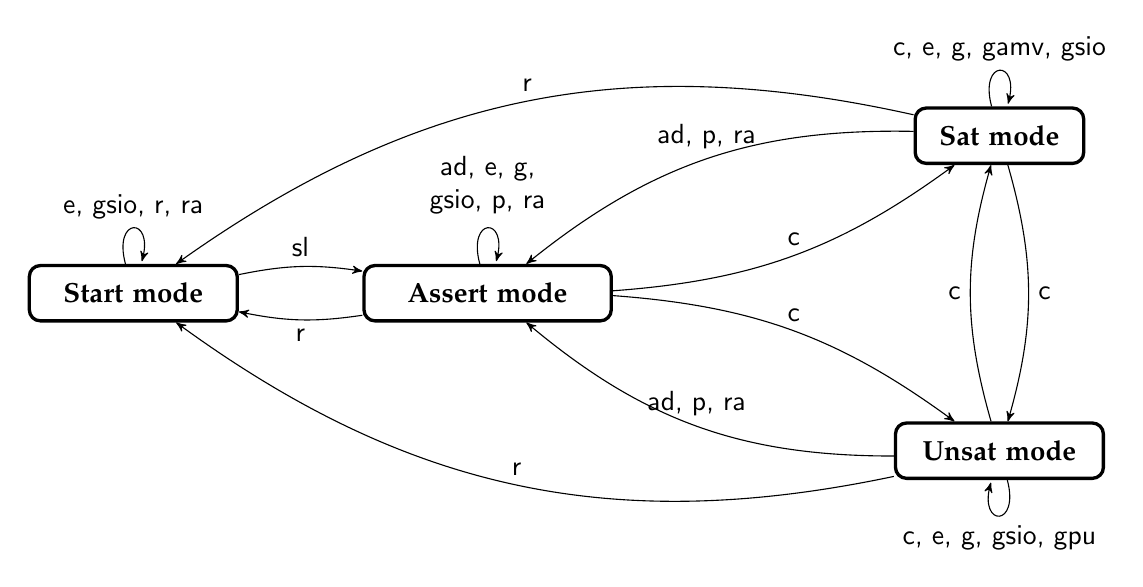
\begin{tikzpicture}[->,>=stealth']
 \node[state,    	% layout (defined above)
  text width=2.5cm, 	% distance to ASSERT
  yshift=2cm, 		% move 2cm in y
  anchor=center] (START) 
 {\textbf{Start mode}};
  
 \node[state,    	% layout (defined above)
  text width=3cm,
%  yshift=2cm, 		% move 2cm in y
  right of=START, 	% Position is to the right of ASSERT
  node distance=4.5cm, 	% distance to ASSERT
  anchor=center] (ASSERT) 
 {\textbf{Assert mode}};
  
 % State: SAT with different content
 \node[state,    	% layout (defined above)
  text width=2cm, 	% max text width
  yshift=2cm, 		% move 2cm in y
  right of=ASSERT, 	% Position is to the right of ASSERT
  node distance=6.5cm, 	% distance to ASSERT
  anchor=center] (SAT) 	% posistion relative to the center of the 'box'
 {\textbf{Sat mode}};
 
 % STATE UNSAT
 \node[state,
  below of=SAT,
  yshift=-3cm,
  anchor=center,
  text width=2.5cm] (UNSAT) 
 {\textbf{Unsat mode}};

 % draw the paths and and print some Text below/above the graph
 \path 
 (START)	edge[loop above]	node[anchor=north,above]{\sf e, gsio, r, ra} (START)
 (START)	edge[bend left=10]	node[anchor=north,above]{\sf sl} (ASSERT)

 (ASSERT)	edge[loop above]	node[anchor=north,above]{\sf \begin{tabular}{c} ad, e, g, \\ gsio, p, ra\end{tabular}} (ASSERT)
 (ASSERT)	edge[bend right=16]	node[anchor=south,above]{\sf c} (SAT)
 (ASSERT)	edge[bend left=16]	node[anchor=north,above]{\sf c} (UNSAT)
 (ASSERT)	edge[bend left=10]	node[anchor=south,below]{\sf r} (START)

 (SAT)		edge[loop above]	node[anchor=south,above]{\sf c, e, g, gamv, gsio} (SAT)
 (SAT)		edge[bend right=24]	node[anchor=south,above]{\sf r} (START)
 (SAT)		edge[bend right=20]	node[anchor=south,above]{\sf ad, p, ra} (ASSERT)
 (SAT)		edge[bend left=16]	node[anchor=south,right]{\sf c} (UNSAT)

 (UNSAT)	edge[loop below]	node[anchor=north,below]{\sf c, e, g, gsio, gpu} (UNSAT)
 (UNSAT)	edge[bend left=24]	node[anchor=south,above]{\sf r} (START)
 (UNSAT)	edge[bend left=20]	node[anchor=south,above]{\sf ad, p, ra} (ASSERT)
 (UNSAT)	edge[bend left=16]	node[anchor=south,left]{\sf c} (SAT)
 ;
\end{tikzpicture}
\end{center}
%
Command name abbreviations:
{\scriptsize
\medskip

\begin{multicols}{2}
\begin{tabular}{r@{\ \ }c@{\ \ }l}
{\sf ad} & = & \ter{assert}, \ter{declare-}{*}, \ter{define-}{*}
\\ 
{\sf c} & = & \ter{check-sat}{*} 
\\ 
{\sf e} & = & \ter{echo} \\ 
{\sf g} & = & \ter{get-assertions} \\ 
{\sf gamv} & = & \ter{get-assignment}, \ter{get-model}, \ter{get-value} \\
{\sf gsio} & = & \ter{get-info}, \ter{get-option}, \ter{set-info}, \ter{set-option} \\  
\end{tabular}

\begin{tabular}{r@{\ \ }c@{\ \ }l}
{\sf gpu} & = & \ter{get-proof}, \ter{get-unsat-}{*} \\ 
{\sf p} & = & \ter{pop}, \ter{push} \\ 
{\sf r} & = & \ter{reset} \\ 
{\sf ra} & = & \ter{reset-assertions} \\ 
{\sf sl} & = & \ter{set-logic}
\end{tabular}
\end{multicols}
}
\caption{Abstract view of transitions between solver execution modes.
The symbol * here stands for the matching wildcard.
}

\label{fig:modes}
\end{figure}


At a high-level, a compliant solver can be understood as being at all times 
in one of four \define{execution modes}:
a \mode{start} mode, an \mode{assert} mode and two \define{query} modes, 
\mode{sat} and \mode{unsat}.
The solver starts in \mode{start} mode, moves to \mode{assert mode} 
once a logic is set, and then moves to one of the two query modes 
after executing a check command.
Any command other than \ter{reset} that modifies the assertion stack brings 
the solver back from a query mode to the \mode{assert} mode.
The \ter{reset} command takes the solver back to \mode{start} mode.

The transition system in Figure~\ref{fig:modes} illustrates 
in some detail which commands can trigger which mode transitions.
The set of labels for each transition describes the commands that may cause it.
With the exception of \ter{exit}, 
if a command does not appear on any transitions originating from a mode,
it is not permitted in that mode.
The \ter{exit} command, which causes the solver to quit, can be issued in any mode.

The solver must respond with an error when given a command not permitted 
in the current mode.
Because of its level of abstraction, the transition system diagram 
in Figure~\ref{fig:modes} does not specify the conditions under which 
a specific command causes a transition to one mode as opposed to another;
see Section~\ref{sec:commands} for details on that.
Similarly, the diagram does not account for the fact that some specific options
can be set only in certain modes. 
Such restrictions are described in Section~\ref{sec:options}. 

%-------------------------------------------------------------------------------
\subsection{Solver responses} \label{sec:response}
%-------------------------------------------------------------------------------

Regular output, including responses \emph{and errors}, produced 
by compliant solvers should be written to the \define{regular} output channel.
Diagnostic output, including warnings, debugging, tracing, 
or progress information, should be written to the \define{diagnostic} output channel.
These channels may be set with the \nter{set-option} command 
(see Section~\ref{sec:options} below).  
By default they are the standard output and standard error channels, 
respectively.

Generally, once a solver completes its processing in response to a command, 
it should print to its regular output channel a \nter{general\_response}:

\begin{center}
 \begin{tabular}{lll}
  \cGeneralResponse
 \end{tabular}
\end{center}

\noindent 
The value \ter{success} is the default response for a successful execution
of a supported command.  
A number of commands have a more detailed response in place of \ter{success}, 
discussed in Section~\ref{sec:commands} for each of them.
The value \ter{unsupported} should be returned if the command 
or some specific input to it is not supported by the solver.
An expression of the form \expr{(error $e$)} should be returned for any 
kind of error situation (wrong command syntax, incorrect parameters, 
erroneous execution, and so on).
The value of $e$ is a solver-specific string containing 
a message that describes the problem encountered.\footnote{%
Returning the empty string is allowed but discouraged 
because of its uninformative content.
}

Any response which is not double-quoted and not parenthesized must be followed 
by at least one whitespace character (for example, a new line character).\endnote{
This enables applications reading a compliant solver's response to know 
when an identifier (like \ter{success}) has been completely printed and,
in general, when the solver has completed processing a command. 
For example, this is needed if one wants to use an off-the-shelf 
S-expression parser (e.g., \texttt{read} in Common Lisp) to read responses.
}

Several options described in Section~\ref{sec:options} below affect the printing 
of responses, in particular by suppressing the printing of \ter{success}, 
or by redirecting the regular or diagnostic output channels.

\paragraph{Errors and solver state.} 
Solvers have two options when encountering errors.  
For both options, they first print an error message 
in the \nter{general\_response} format.  
Then, they may either immediately exit with a non-zero exit status, 
or continue accepting commands.  
In the second case, 
the solver's state remains unmodified by the error-generating command, 
except possibly for timing and diagnostic information.  
In particular, the assertion stack, discussed in Section~\ref{sec:assert-stack}, 
is unchanged.\endnote{
The motivation for allowing these two behaviors is that
the first one (exiting immediately when an error occurs) may be simpler to implement,
while the latter may be more useful for applications, though it might be 
more burdensome to support the semantics of leaving the state unmodified 
by the erroneous command.
}

The predefined \attr{error-behavior} attribute can be used 
with the $\ter{get-info}$ command to check which error behavior 
the tool supports (see Section~\ref{sec:get-info} below).

%-------------------------------------------------------------------------------
\subsection{Printing of terms and defined symbols} 
%-------------------------------------------------------------------------------
Several commands request the solver to print sets of terms.  
While some commands, naturally, place additional semantic requirements on these sets, 
the general syntactic requirement is that output terms must be well-sorted 
with respect to the current signature (as defined below in Section~\ref{sec:assert-stack}).
%
%ct remove this because get-rank is out for the time being
%If the signature is expanded, due to
%the introduction of new symbols during solving, then the ranks of
%those new symbols can be obtained with $\akey{get-rank}$.

All output from a compliant solver should print any symbols
defined with \ter{define-sort} and \ter{define-fun} just as they are, 
without replacing them by the expression they are defined to be equal to.  
This approach generally keeps the output from solvers much more compact than 
it would be if definitions were expanded.

%ct removed for now, we need to agree on the format for this
%
%\paragraph{Getting a symbol's rank.} The $\akey{get-rank}$ command allows
%the calling environment to request the sort of a symbol.  In case the
%symbol is overloaded, all ranks should be returned.  This command is
%likely to be particularly useful to determine the sort of
%solver-introduced symbols.



%-------------------------------------------------------------------------------
\subsection{The assertion stack} \label{sec:assert-stack}
%-------------------------------------------------------------------------------

A compliant solver maintains a stack of sets, 
each of which consists of \define{assertions}.
Assertions are formulas, declarations, and definitions.
We will use the following terminology with regards to this data structure:
\begin{itemize}
\item 
\define{assertion stack:} the single stack of sets of assertions;
\item 
\define{assertion level:} an element of the assertion stack 
(i.e., a set of assertions);
\item 
\define{context:} the union of all the assertion levels on the assertion stack
together with any global declarations (see Section~\ref{sec:decl-defn});
\item 
\define{current assertion level:} the assertion level at the top of the stack 
(i.e., the most recent);
\item \define{first assertion level:} the first assertion level in the stack
(i.e., the least recent);
\item \define{current signature:} the signature determined by the logic
  specified with the most recent \ter{set-logic} command and
by the set of sort symbols and rank associations (for function symbols) 
in the current context.  
\end{itemize}

Initially, when the solver starts, the assertion stack consists 
of a single element, the first assertion level, which is empty.
While new assertions can be added to this set, the set itself cannot be removed 
from the stack with a pop operation.
The following commands modify the current context:
\begin{quote}
\ter{assert},
\ter{declare-sort}, \ter{declare-fun},
\ter{declare-const},
\ter{define-sort}, \ter{define-fun}, 
\ter{define-fun-rec}, \ter{define-funs-rec},
\ter{pop}, \ter{push},
\ter{reset}, and \ter{reset-assertions}.
\end{quote}
%\footnote{%
%A \ter{check-sat-assuming} command modifies the context by temporarily asserting
%some formulas as \define{assumptions} (see Section~\ref{sec:checking-for-sat}).
%}

%-------------------------------------------------------------------------------
\subsection{Symbol declarations and definitions}\label{sec:decl-defn}
%-------------------------------------------------------------------------------

A number of commands allow the declaration or definition of a function 
or sort symbol.  
By default, these declarations and definitions are added to the current
assertion level when the corresponding command is executed.
Popping that assertion level removes them.\endnote{
It is desirable to have the ability to remove declarations and definitions, 
for example if they are no longer needed at some point during an interaction 
with a solver (so that the memory required for them can be reclaimed), or 
if a defined symbol needs to be redefined.  
The current approach of allowing declarations and definitions to be 
locally scoped supports removal by popping the containing assertion level.
Other approaches, such as the ability to add shadowing declarations or
definitions of symbols, or to ``undefine'' or ``undeclare'' them, 
present some issues: for example, how to print symbols that have been shadowed, 
undefined or undeclared.
As a consequence, they are not supported in the language.
}
As an alternative, declarations and definitions can all be made \define{global} 
by running the solver with the option \attr{global-declarations} set to \ter{true}.
When running with this option set, all declarations and definitions become permanent.
That is, they survive any pop operations on the assertion stack as well as invocations
of \ter{reset-assertions} and can only be removed by a global reset, 
achieved with the \ter{reset} command.\endnote{
Setting \attr{global-declarations} to \ter{true} can be understood as stating 
that declarations and definitions are not part of the assertion stack, 
and so resetting the stack has no impact on them. 
This option is convenient in applications that benefit from using push and pop
for assertions but need to continue using symbols declared after a push 
even after the corresponding pop.
}

Well-sortedness checks, required for commands that use sorts or terms, 
are always done with respect to the current signature.
It is an error to declare or define a symbol
that is already in the current signature.
This implies in particular that, contrary to theory function symbols,
user-defined function symbols cannot be overloaded.\endnote{
The motivation for not overloading user-defined symbols is to simplify 
their processing by a solver.
This restriction is significant only for users 
who want to extend the signature of the theory used by a script 
with a new polymorphic function symbol---i.e., one whose rank would contain
parametric sorts if it was a theory symbol.
For instance, users who want to declare a ``reverse'' function 
on arbitrary lists, must define a different reverse function symbol 
for each (concrete) list sort used in the script.
This restriction might be removed in future versions.
}


%-------------------------------------------------------------------------------
\subsection{In-line definitions}\label{sec:inline-defn}
%-------------------------------------------------------------------------------

Any closed subterm $t$ occurring in the argument(s) of a command $c$
can be optionally annotated with a \attr{named} attribute; that is, it
can appear as \expr{(!~$t$ \attr{named} $f$)} where $f$ is a fresh function symbol
from \nter{symbol}.
For such a command $c$, let
\begin{center}
\expr{(!~$t_1$ \attr{named} $f_1$)}, \ldots, \expr{(!~$t_n$ \attr{named} $f_n$)}
\end{center}
%
be the enumeration of all the named subterms of $c$ obtained by the (depth-first) left-to-right post-order traversal of $c$.
The semantics of the command $c$ is the same as the sequence of commands
\begin{center}
\begin{tabular}{l}
 \expr{(define-fun $f_1$ () $\sigma_1$ $t_1'$)} \\
 \vdots \\
 \expr{(define-fun $f_n$ () $\sigma_n$ $t_n'$)} \\
 $c'$
\end{tabular}
\end{center}
%
where, for each $i=1,\ldots,n$, 
$(i)$ $\sigma_i$ is the sort of $t_i$ with respect to the current signature 
up to the declaration of $f_i$,
$(ii)$ $t_i'$ is the term obtained from $t_i$ by removing 
all its \attr{named} annotations, and 
$(iii)$ $c'$ is similarly obtained from $c$ by removing 
all its \attr{named} annotations.

By these semantics, each \define{label} $f_i$ can occur, as a constant symbol, 
in any subexpression of $c$ that comes after \expr{(!~$t_i$ \attr{named} $f_i$)} 
in the left-to-right post-order traversal of $c$, as well as after the command $c$ itself.
The labels $f_1, \ldots, f_n$ can be used like any other user-defined nullary
function symbols, with the same visibility and scoping restrictions 
they would have if they had been defined with the sequence of commands above. 
However, contrary to function symbols introduced by \expr{define-fun},
labels have an additional, dedicated use in the commands 
\expr{get-assignment} and \expr{get-unsat-core}
(see Section~\ref{sec:commands}).


%------------------------------------------------------------------------
\subsection{Solver options} \label{sec:options}
%------------------------------------------------------------------------

Solver options may be set using the \ter{set-option} command, and
their current values can be obtained using the \ter{get-option} command.  
If a solver does not support the setting of a particular option,
for either command it should output \ter{unsupported}.  

Solver-specific option names are allowed and indeed expected.  
A set of standard options is presented in this subsection;
refer to Figure~\ref{fig:command-options} for their format. 
%This version of the language requires solvers to recognize and reply 
%in a standard way only to a few of them, the rest are optional.
We discuss each option below, specifying also their default values and 
whether or not compliant solvers are required to support them. 
It is understood that if a solver does not support one of the optional 
standard options below, it behaves as if that option was permanently
set to its default value. 

Some options can be set only when the solver is in \mode{start} mode.
We list the mode when that is the case.
Attempting to set an option when the solver is not in a permitted mode 
should trigger an error response.
Each option starting with the \ter{produce-} prefix is a Boolean option
that enables a specific command.
When such an option is set to \ter{false}, calling the corresponding
command should trigger an error response.

The set of standard options is likely to be expanded or otherwise revised 
as further desirable common options and kinds of information across tools
are identified.  

\begin{description}

\item[\attr{diagnostic-output-channel}] 
\quad default: \ter{"stderr"}
\quad support: required
\\
The argument is a string consisting of the name of a file to be used subsequently 
as the diagnostic output channel.
The input value \ter{"stderr"} is interpreted specially to mean 
the solver's standard error channel.  
With other filenames, subsequent solver output is to be appended to the named file 
(and the file should be first created if it does not  already exist).

\item[\attr{global-declarations}] 
\quad default: \ter{false}
\quad support: optional
\quad mode: \mode{start}
\\
If the solver supports this option, setting it to \ter{true} causes all
declarations and definitions to be global (permanent) as opposed to being added
to the current assertion level.

\item[\attr{interactive-mode}] 
\quad default: \ter{false}
\quad support: optional
\quad mode: \mode{start}
\\
The old name for \ter{produce-assertions}. 
Deprecated.

\item[\attr{print-success}] 
\quad default: \ter{false}
\quad support: required
\\
Setting this option to \ter{true} causes the solver to print 
\ter{success} as a response to commands.  
Other output remains unchanged.

\item[\attr{produce-assertions}] 
\quad default: \ter{false}
\quad support: optional
\quad mode: \mode{start}
\\
If the solver supports this option, setting it to \ter{true} enables 
the \ter{get-assertions} command.
This option was called \ter{interactive-mode} in previous versions.

\item[\attr{produce-assignments}] 
\quad default: \ter{false}
\quad support: optional
\quad mode: \mode{start}
\\
If supported, this enables the command \ter{get-assignment}.  

\item[\attr{produce-models}] 
\quad default: \ter{false}
\quad support: optional
\quad mode: \mode{start}
\\
If supported, this enables the commands \ter{get-value} and \ter{get-model}.  

\item[\attr{produce-proofs}] 
\quad default: \ter{false}
\quad support: optional
\quad mode: \mode{start}
\\
If supported, this enables the command \ter{get-proof}.  

\item[\attr{produce-unsat-assumptions}] 
\quad default: \ter{false}
\quad support: optional
\quad mode: \mode{start}
\\
If supported, this enables the command \ter{get-unsat-assumptions}.  

\item[\attr{produce-unsat-cores}] 
\quad default: \ter{false}
\quad support: optional
\quad mode: \mode{start}
\\
If supported, this enables the command \ter{get-unsat-core}.  

\item[\attr{random-seed}] 
\quad default: $0$
\quad support: optional
\quad mode: \mode{start}
\\
The argument is a numeral for the solver to use as a random seed,
in case the solver uses (pseudo-)randomization.
The default value of $0$ means that the solver can use any random seed---possibly 
even a different one for each run of the same script.
The intended use of the option is to force the solver to produce identical results 
whenever given identical input (including identical non-zero seeds) on repeated runs of the solver.

\item[\attr{regular-output-channel}] 
\quad default: \ter{"stdout"}
\quad support: required
\\
The argument should be a filename to use subsequently for
the regular output channel.  The input value \ter{"stdout"} is interpreted
specially to mean the solver's standard output channel.
With other filenames, subsequent solver output is to be appended to the named file 
(and the file should be first created if it does not  already exist).

\item[\attr{reproducible-resource-limit}] 
\quad default: $0$
\quad support: optional
\\
If the solver supports this option, setting it to $0$ disables it.
Setting it a non-zero numeral $n$ will cause each subsequent check command 
to terminate within a bounded amount of time dependent on $n$.
The internal implementation of this option and its relation to run time or 
other concrete resources can be solver-specific.
However, it is required that the invocation of a check command return 
\ter{unknown} whenever the solver is unable to determine the satisfiability 
of the formulas in the current context within the current resource limit. 
Setting a higher value of $n$ should allow more resources to be used, 
which may cause the command to return \ter{sat} or \ter{unsat} instead 
of \ter{unknown}. 
Furthermore, the returned result should depend deterministically on $n$;
specifically, it should be the same every time the solver is run 
with the same sequence of previous commands on the same machine 
(and with an arbitrarily long external time out). 
If the solver makes use of randomization, it may require 
the \attr{random-seed} option to be set to a value other than $0$ 
before \attr{reproducible-resource-limit} can be set to a positive value.\endnote{
Note that this option is not intended to be used for comparisons
between different solvers since they can implement it differently.
Its purpose is simply to guarantee the reproducibility 
of an individual solver's results under the same external conditions.
}

\item[\attr{verbosity}] 
\quad default: no standard default value
\quad support: optional
\\
The argument is a numeral controlling the level of diagnostic output produced
by the solver.  
All such output should be written to the diagnostic output channel\endnote{
This is to avoid confusion with the responses to commands,
which are written to the regular output channel.  
}
which can be set and later changed via the \ter{diagnostic-output-channel} option.  
An argument of $0$ requests that no such output be produced.  
Higher values correspond to more verbose output.
\end{description}

%---------------------------------------------------------------------------
\subsection{Solver information}   \label{sec:get-info}
%---------------------------------------------------------------------------

The format for responses to \ter{get-info} commands,
both for standard and solver-specific information flags,
is defined by the \nter{get\_info\_response} category 
in Figure~\ref{fig:command-responses}.
The standard \ter{get-info} flags and specific formats 
for their corresponding responses are given next.  

\begin{description}

\item[\attr{all-statistics}] 
\quad support: optional
\quad mode: \mode{sat}, \mode{unsat}
\\
Solvers reply with a parenthesis-delimited sequence of \nter{info\_response} 
values (see Figure~\ref{fig:command-responses}) providing various statistics 
on the execution of the most recent check command.
No standard statistics are defined for the time being,\endnote{
Some commonly used statistics 
(e.g., number of restarts of a solver's propositional reasoning engine)
are difficult to define precisely and generally, 
while the exact semantics of others, such as time and memory usage,
have not being agreed upon yet by the SMT community.
}
so they are all solver-specific.
%ct reworded
%Any call to \ter{get-info} with \attr{all-statistics} must follow 
%a check command and precede any commands that modify the assertion stack.  
Executions of \ter{get-info} with \attr{all-statistics} are allowed only
when the solver is in \mode{sat} or \mode{unsat} mode.

\item[\attr{assertion-stack-levels}]
\quad support: optional
\\
The response is a pair of the form
\expr{(\attr{assertion-stack-levels} $n$)}
where $n$ is a numeral indicating the current number of levels 
in the assertion stack besides the first assertion level.\endnote{
This command is useful for interactive use,
to keep track of the current number of nested \ter{push} commands.
}

\item[\attr{authors}] 
\quad support: required
\\
The response is a pair of the form
\expr{(\attr{authors} $s$)}
where $s$ is a string literal listing the names of the solver's authors.

\item[\attr{error-behavior}]
\quad support: required
\\  
The response is a pair of the form
\expr{(\attr{error-behavior} $r$)}
where $r$ is either \ter{immediate-exit} or \ter{continued-execution}.
A response of \ter{immediate-exit} indicates that the solver
will exit immediately when an error is encountered.  
A response of \ter{continued-execution} indicates that when an error is
encountered, the solver
will return to the state it was in immediately before the command triggering
the error, and continue 
accepting and executing new commands.  
See Section~\ref{sec:response} for more information.

\item[\attr{name}]
\quad support: required
\\
The response is a pair of the form
\expr{(\attr{name} $s$)}
where $s$ is a string literal with the name of the solver.

\item[\attr{reason-unknown}]
\quad support: optional
\quad mode: \mode{sat}
\\
%ct reworded
%Any call to \ter{get-info} with \attr{reason-unknown} must follow a check command
%whose response was \ter{unknown}.  In addition, there must be no intervening commands 
%that modify the assertion stack.
Executions of \ter{get-info} with \attr{reason-unknown} are allowed only
when the solver is in \mode{sat} mode following a check command
whose response was \ter{unknown}.
%
The response is a pair of the form
\expr{(\attr{reason-unknown} $r$)}
where $r$ is an element of \nter{reason\_unknown} giving a short reason 
why the solver could not successfully check satisfiability.
In general, this reason can be provided by a solver-defined s-expression.
Two predefined s-expressions are
\ter{memout}, for out of memory, and \ter{incomplete}, which indicates 
that the solver knows it is incomplete for the class of formulas containing 
the most recent check query.

\item[\attr{version}]
\quad support: required
\\ 
The response is a string literal with the version number of the solver 
(e.g., \texttt{"1.2"}).
\end{description}


%-------------------------------------------------------------------------------
\section{Commands} \label{sec:commands}
%-------------------------------------------------------------------------------

The full set of commands and their expected behavior are described 
in this section.
Commands may impose restrictions on their arguments as well as restrictions 
on when they can be issued.
Unless otherwise specified, the solver is required to produce an error 
when any of these restrictions is violated.
Figure~\ref{fig:modes} describes the commands permitted in each execution mode 
and the mode transitions each command may trigger.
We specify below the conditions under which a command triggers one mode transition 
versus another only for commands that may trigger more than one transition. 

%-------------------------------------------------------------------------------
\subsection{(Re)starting and terminating} \label{sec:restarting}
%-------------------------------------------------------------------------------

\begin{description}

%%% reset %%%
%
\item[\expr{(reset)}]
resets the solver completely to the state it had after it was started
and before it started reading commands.\endnote{
This allows the user to reset the state of the solver 
without paying the cost of restarting it.
}
\smallskip

%%% set-logic %%%
%
\item[\expr{(set-logic $l$)}]
tells the solver what logic, in the sense of Section~\ref{sec:logics},
is being used.
The argument $l$ can be the name of a logic in the SMT-LIB catalog or 
of some other solver-specific logic.
The effect of the command is to add globally (and permanently)
a declaration of each sort and function symbol in the logic.

The argument $l$ can also be the predefined symbol \ter{ALL}.
With this argument, the solver sets the logic to the most general logic 
it supports.\endnote{
Having \ter{ALL} is convenient for client applications that generate 
problems on the fly in a variety of logics supported by some specific solver
without knowing in advance the specific logic for each problem.
SMT-LIB scripts meant for the SMT-LIB library should not use \ter{ALL} 
in set-logic but should instead use a specific logic name.
}
Note that while the reaction to \expr{(set-logic ALL)} is the same 
for every compliant solver, the chosen logic is solver-specific.

We refer to the logic set by the most recent \ter{set-logic} command as 
the \define{current logic}.
\smallskip

%%% set-option %%%
%
\item[\expr{(set-option $o$ $v$)}]
sets a solver's option $o$ to a specific value $v$.
More details on predefined options and required behavior are provided 
in Section~\ref{sec:options}.  
In general, if a solver does not support the setting of a particular option,
its response to this command should be \ter{unsupported}.
If the option is one of the predefined ones it should also leave it unchanged 
from its default value.  
The effect of setting a supported option is immediate.
In particular, for options that affect the solver's output, such as 
\attr{diagnostic-output-channel}, \attr{regular-output-channel} and 
\attr{print-success}, 
the effect applies already to the output of the very command 
that is setting the option.

Note that some of the options defined in Section~\ref{sec:options} 
may only be set in \mode{start} mode.\endnote{
The rationale is that a solver may need to make substantial changes 
to its internal configuration to provide the functionality requested 
by these options, and so it needs to be notified before it starts 
processing assertions.
}
\smallskip

%%% exit %%%
%
\item[\expr{(exit)}]
instructs the solver to exit.
\end{description}


%-------------------------------------------------------------------------------
\subsection{Modifying the assertion stack}
%-------------------------------------------------------------------------------

\begin{description}
%%% push %%%
%
\item[\expr{(push $n$)}] 
pushes $n$ empty assertion levels onto the assertion stack.\footnote{%
Typically, $n=1$.
}
If $n$ is $0$, no assertion levels are pushed.
\smallskip

%%% pop %%%
%
\item[\expr{(pop $n$)}] where $n$ is smaller than the number of assertion levels
in the stack, pops the $n$ most-recent assertion levels from the stack.\footnote{%
When $n$ is $0$, no assertion levels are popped.
}
Note that the first assertion level, 
which is not created by a \ter{push} command, 
cannot be popped.
\smallskip

%%% reset-assertions %%%
%
\item[\expr{(reset-assertions)}] removes from the assertion stack 
all assertion levels beyond the first one.
In addition, it removes all assertions from the first assertion level.
Declarations and definitions resulting from the \ter{set-logic} command 
are unaffected (because they are global).
Similarly, if the option \attr{global-declarations} has value \ter{true}
at the time the command is executed, then \emph{all} declarations and definitions
remain unaffected.
Note that any information set with \ter{set-option} commands is preserved 
in any case.

\end{description}


%-------------------------------------------------------------------------------
\subsection{Introducing new symbols} \label{sec:new-symbols}
%-------------------------------------------------------------------------------

\new{The first command below allows the declaration of sort parameters.}
The next seven commands allow one to introduce new sort or function symbols 
by providing them with a rank declaration
(\ter{declare-sort}, \ter{declare-fun} and \ter{declare-const})
or also with a definition 
(\ter{define-sort}, \ter{define-fun}, \ter{define-fun-rec} and 
\ter{define-funs-rec}).
We refer to the former as \define{user-declared} symbols and 
the latter as \define{user-defined} symbols.
Declarations and definitions are made global (permanent) or are added 
to the current assertion level depending on 
whether the option \attr{global-declarations} is set to \ter{true} or not.

\begin{description}

%%% declare-sort-parameter %%%
%
\item[\expr{(declare-sort-parameter $s$)}]
\new{
adds \emph{global} sort parameter $s$ to the current signature.
The command reports an error if $s$ is a sort symbol, sort parameter, 
or theory symbol already present in the current signature.%
}
%\endnote{%
%\new{
%In SMT-LIB 2.7, the \expr{par} construct, short for \emph{parameter}, is a misnomer,
%as \expr{par} actually introduces sort \emph{variables} rather than sort \emph{parameters}.
%We have adopted a pragmatic approach to this issue, 
%deciding not to rename the \expr{par} construct for backward compatibility.
%}
%}
\smallskip

%%% declare-sort %%%
%
\item[\expr{(declare-sort $s$ $n$)}]
adds sort symbol $s$ with associated arity $n$.
It is an error if $s$ is a sort symbol \new{or parameter} already present 
in the current signature.
\smallskip

%%% define-sort %%%
%
\item[\expr{(define-sort $s$ ($u_1$ $\cdots$ $u_n$) $\tau$)}] with $n \geq 0$
adds sort symbol $s$ with arity $n$ and associates it with sort $\tau$,
where the $u_i$'s are (local) sort parameters, and $\tau$ may contain 
any of $u_1$, \dots, $u_n$\new{, but no global sort parameters}.

% (define-sort set-of-pairs (u v) (set (pair (u v))))
% (define-sort set-of-pairs () (set (pair (u v))))
% (set-of-pairs Int Real)

Subsequent well-sortedness checks must treat a sort term like
\expr{($s$ $\tau_1$ $\cdots$ $\tau_n$)} 
as an abbreviation for the term obtained by simultaneously substituting
$\tau_i$ for $u_i$, for $i\in\{1,\ldots,n\}$, in $\tau$.\endnote{
Strictly speaking, only sort symbols introduced with \ter{declare-sort}
expand the initial signature of theory sort symbols.
Sort symbols introduced with \ter{define-sort} do not.
They do not construct \emph{real} sorts,
but \emph{aliases} of sorts built with
theory sort symbols and previously declared sort symbols.
}

The command reports an error
if $s$ is a sort symbol or parameter already present in the current signature or
if $\tau$ is not a well-defined (polymorphic) sort 
with respect to the current signature extended with sort parameters 
$u_1$, \dots, $u_n$.
This restriction prohibits (meaningless) circular definitions
where $\tau$ contains $s$.
\begin{newver}
The $u_i$ sort parameters shadow any previously user-declared sort symbol
or parameter with the same name.
However, they do not shadow theory sort symbols (just as bound variables are
not permitted to shadow declared theory symbols).
The command reports an error if a theory sort
symbol is used as a sort parameter $u_i$.
\end{newver}

\smallskip

%%% declare-fun %%%
%
\item[\expr{(declare-fun $f$ ($\tau_1$ $\cdots$ $\tau_n$) $\tau$)}]
with $n \geq 0$ adds a new symbol $f$ 
with associated rank $\tau_1\cdots\tau_n\tau$.
The command reports an error if a function symbol with name $f$ 
is already present in the current signature.
\new{
Note that 
$\tau_1$ $\cdots$ $\tau_n$, and $\tau$ may contain sort parameters.
In that case $f$ is polymorphic.
}
\smallskip

%%% declare-const %%%
%
\item[\expr{(declare-const $f$ $\tau$)}]
has the same effect as the command \expr{(declare-fun $f$ () $\tau$)}.
\smallskip

%\pfrem{sort parameters in datatypes must come from the par list.}

%\pfrem{using declared sort parameters only make sense in assertions.
%  We need order elsewhere.}
%%% declare-datatypes %%%
%
\item[%
\expr{(declare-datatypes (($\delta_1$ $k_1$) $\cdots$ ($\delta_n$ $k_n$))
                         ($d_1$ $\cdots$ $d_n$))}]
with $n > 0$ introduces $n$ algebraic datatypes $\delta_1,\dots,\delta_n$
with respective arities $k_1,\dots,k_n$ and declarations $d_1,\dots,d_n$. 
Let $\delta = \delta_i$, $k = k_i$ and $d = d_i$ for $i \in \{1,\ldots,n\}$.
If $k >0$ then $d$ is an expression of the form 
\expr{(par ($u_1$ $\cdots$ $u_k$) $l$)}
where $u_1, \ldots, u_k$ are sort parameters;\endnote{
\new{
Using local sort parameters as opposed to globally declared sort parameters
is necessary because their order is meaningful, as arguments of the sort constructor.
}
}
% The u_1, u_k correspond to the k arguments of the sort constructor.  
% (Pair Int Real) is not the same of (Pair Real Int), and the relation to the pair
% constructor and the order of arguments in the pair constructor is set through
% the order of the sort parameters in par
otherwise, it is just $l$. 
In either case, $l$ is a (parenthesis-delimited) list of \emph{one or more} 
expressions of the form
%
\begin{center}
 \expr{($c$ ($s_1$ $\tau_1$) $\cdots$ ($s_m$ $\tau_m$))},
\end{center}
where 
$(i)$ $m \geq 0$, 
$(ii)$ $c$ is a symbol, a \define{constructor for $\delta$}, and 
$(iii)$ for each $j=1,\ldots,m$, $s_j$ is a symbol, a \define{selector for $c$}, and 
$(iv)$ $\tau_j$ is a sort term
that contains no occurrences of $\delta_1, \ldots, \delta_n$ below its top symbol.

In the polymorphic case,
\new{the terms $\tau_i$ can contain only the sort parameters in the list $u_1, \ldots, u_k$}.%
\footnote{%
\new{
No previously declared sort parameter that is not shadowed by a $u_i$ can be used.
}
}
The datatype $\delta$ must be \define{well founded} in the following inductive sense:
it must have a constructor of rank $\tau_1\cdots\tau_m\delta$ 
such that $\tau_1\cdots\tau_m$ does not contain any of the datatypes 
from $\{\delta_1, \ldots, \delta_n\}$ or, if it does contain some, they are well founded.

A compliant solver must return an error in response to invocations of this command 
that do not satisfy all of the restrictions above.  

In the polymorphic case, 
the command has the effect of declaring each $\delta$ as a sort symbol of arity $k$;
each constructor $c$ as a function symbol of parametric rank $\tau_1\cdots\tau_m\delta$;
and each $s_i$ as a function symbol of parametric rank $\delta\tau_i$.
The monomorphic case is analogous.

Note that the sort terms $\tau_1, \ldots,\tau_m$ can contain any previously defined 
sort symbol as well as any of the datatypes $\delta_1, \ldots, \delta_n$,
as long as those datatypes are well founded.\endnote{
The input of this command is split in two arguments precisely to facilitate
the type-checking of the sort terms $\tau_1, \ldots,\tau_m$.
The first argument makes sure that when it is time to parse these terms
each symbol $\delta_i$ is known to be a sort symbol of arity $k_i$.
}
This allows the declaration of recursive and mutually recursive datatypes.\endnote{
The various restrictions on the definition of a datatype $\delta$ are crucial 
since they allow the existence of standard interpretations for $\delta$.
See Chapter~\ref{chap:logical-semantics} for more details.
}

On successfully executing this command, 
for each constructor $c$ in a declared datatype $\delta$, 
the solver will also automatically declare a \define{tester}
with rank $\delta\,\ter{Bool}$.
The tester's name is an indexed identifier (see Section~\ref{sec:identifiers}) 
of the form \expr{(\_ is $c$)}.
\medskip

\begin{lstlisting}[linewidth=37em]
; an enumeration datatype
(declare-datatypes ( (Color 0) ) (
  ( (red) (green) (blue) ))
)
; testers: (_ is red), (_ is green)

; integer lists with "empty" and "insert" constructors
(declare-datatypes ( (IntList 0) ) (
  ( (empty) (insert (head Int) (tail IntList) )))
)
; testers: (_ is empty), (_ is insert)

; parametric lists with "nil" and "cons" constructors
(declare-datatypes ( (List 1) ) (
  (par (T) ( (nil) (cons (car T) (cdr (List T)) )))))

; option datatype
(declare-datatypes ( (Option 1) ) (
  (par (X) ( (none) (some (val X)) ))))

; parametric pairs
(declare-datatypes ( (Pair 2) ) (
  (par (X Y) ( (pair (first X) (second Y)) ))))
  
; two mutually recursive datatypes
(declare-datatypes ( (Tree 1) (TreeList 1) ) (
  ; Tree
  (par (X) ( (node (value X) (children (TreeList X)) )))
  ; TreeList
  (par (Y) ( (empty) 
    (insert (head (Tree Y)) (tail (TreeList Y))) ))))
    
\end{lstlisting}

Since $\delta_1, \ldots, \delta_n$ are sort symbols, 
none of them can be a previously declared sort symbol.
Similarly, constructors and selectors are function symbols,
so none of them can be a previous declared/defined function symbol.
This has the effect of also prohibiting, for instance, the use 
of the same constructor in different datatypes or the use 
of repeated instances of the same selector in the same datatype.\endnote{
The rationale for this restriction is the same as for function symbols
introduced with \ter{declare-fun} and \ter{define-fun}, i.e., 
keep parsing and type checking simple. 
}
\smallskip

%%% declare-datatype %%%
%
\item[\expr{ 
(declare-datatype $\delta$ $d$)}] is an abbreviation of 
\begin{center}
\expr{(declare-datatypes (($\delta$ $0$)) ($d$))} 
\end{center}
if $\delta$ is not parametric, and an abbreviation of 
\begin{center}
\expr{(declare-datatypes (($\delta$ $k$)) ($d$))} 
\end{center}
if $d$ has the form \expr{(par ($u_1$ $\cdots$ $u_k$) $l$)}.
This command provides a simpler syntax for defining a single datatype.

\begin{lstlisting}[linewidth=37em]
; an enumeration datatype
(declare-datatype Color ( (red) (green) (blue) ))

(declare-datatype IntList 
  ( (empty) 
    (insert (head Int) (tail IntList) )))

(declare-datatype List (par (E)
  ( (nil) 
    (cons (car E) (cdr (List E)) ))))

(declare-datatype Option (par (X) 
  ( (none) 
    (some (val X) ))))

(declare-datatype Pair (par (X Y)
 ( (pair (first X) (second Y)) ))))
\end{lstlisting}
\smallskip

%%% define-fun %%%
%
\item[\expr{(define-fun $f$ (($x_1$ $\tau_1$) $\cdots$ ($x_n$ $\tau_n$)) $\tau$ $t$)}]
with $n \geq 0$ and $t$ not containing $f$ is 
semantically equivalent to the command sequence

\begin{tabular}{l}
\expr{(declare-fun $f$ ($\tau_1$ $\cdots$ $\tau_n$) $\tau$)} \\
\expr{(assert (forall (($x_1$ $\tau_1$) $\cdots$ ($x_n$ $\tau_n$)) 
       (= ($f$ $x_1$ $\cdots$ $x_n$) $t$))}.
\end{tabular}

%but differs in that $f$ is considered a definition and will be expanded in
%solver output if the \attr{expand-definitions} option is set to \ter{true}.
Note that the restriction on $t$ prohibits recursive or mutually recursive 
definitions, 
which are instead provided by \ter{define-fun-rec} and \ter{define-funs-rec}.
The command reports an error if a function symbol with name $f$ is already 
present in the current signature or if the argument $t$ is not a well-sorted term 
of sort $\tau$ with respect to the current signature extended 
with the sort associations $(x_1:\tau_1),\; \ldots,\; (x_n:\tau_n)$.
\smallskip

%%% define-const %%%
%
\new{
\item[\expr{(define-const $f$ $\tau$ $t$)}] has the same effect as
\expr{(define-fun $f$ () $\tau$ $t$)}.
\smallskip
}

%%% define-funs-rec %%%
%
\item[\expr{(define-funs-rec ($d_1$ $\cdots$ $d_m$) ($t_1$ $\cdots$ $t_m$))},]
where $m > 0$ and for $i=1,\ldots,m$,
$d_i$ has the form
\begin{center}
\expr{($f_i$ (($x_{i,1}$ $\tau_{i,1}$) $\cdots$ ($x_{i,n_i}$ $\tau_{i,n_i}$)) $\tau_i$)}
\end{center}
with 
$n_i \geq 0$ and $f_1, \ldots, f_m$ pairwise distinct,
is semantically equivalent to the command sequence 
\smallskip

{\small
\begin{tabular}{l}
\expr{(declare-fun $f_1$ ($\tau_{1,1}$ $\cdots$ $\tau_{1,n_1}$) $\tau_1$)} 
\\
\hspace{10em} \vdots 
\\
\expr{(declare-fun $f_m$ ($\tau_{m,1}$ $\cdots$ $\tau_{m,n_m}$) $\tau_m$)} 
\\
\expr{(assert (forall (($x_{1,1}$ $\tau_{1,1}$) $\cdots$ ($x_{1,n_1}$ $\tau_{1,n_1}$)) 
       (= ($f_1$ $x_{1,1}$ $\cdots$ $x_{1,n_1}$) $t_1$))}
\\
\hspace{16em} \vdots 
\\
\expr{(assert (forall (($x_{m,1}$ $\tau_{m,1}$) $\cdots$ ($x_{m,n_m}$ $\tau_{m,n_m}$)) 
       (= ($f_m$ $x_{m,1}$ $\cdots$ $x_{m,n_m}$) $t_m$))} .
\end{tabular}
}
\smallskip

This command can be used to define multiple functions recursively,
in particular, mutually recursively.\endnote{
Similar to \ter{define-fun}, while strictly not needed, 
\ter{define-funs-rec} provides a more structured way to define functions axiomatically,
as opposed to introducing a new function with \ter{declare-fun} and then 
providing its definition with \ter{assert} and a quantified formula.
This gives an SMT solver the opportunity to easily recognize 
function definitions and possibly process them specially.
}
Mutual recursion is possible since each term $t_i$ can contain any applications 
of $f_1, \ldots, f_m$.  

Note that, according to the semantics above, \ter{define-funs-rec} imposes 
no requirements that each $f_i$ be terminating
(a meaningless notion in our context) or even well-defined.\footnote{%
In fact, it is even possible, although certainly not desirable, 
to have a definition like
\expr{(define-funs-rec ((f ((x Bool)) Bool)) ((not (f x))) )},
which makes the set of formulas in the context unsatisfiable.
}
The only requirement is on the well-sortedness of the definitions.

The command reports an error if for any $i \in \{1,\ldots,m\}$ 
a function symbol with name $f_i$ is already present in the current signature 
or if $t_i$ is not a well-sorted term of sort $\tau_i$ with respect 
to the current signature extended with the sort associations 
$(f_1:\tau_{1,1}\; \cdots\; \tau_{1,n_1}\tau_1)$, \ldots,
$(f_m:\tau_{m,1}\; \cdots\; \tau_{m,n_m}\tau_m)$
and
$(x_{i,1}:\tau_{i,1}),\; \ldots,\; (x_{i,n_i}:\tau_{i,n_i})$.

\new{
Note that, for each $i$, $\tau_{i,1}$ $\cdots$ $\tau_{i,n_i}$, and $\tau_i$ may contain sort parameters.
In that case $f_i$ is polymorphic. }

\smallskip

%%% define-fun-rec %%%
%
\item[\expr{(define-fun-rec $f$ (($x_1$ $\tau_1$) $\cdots$ ($x_n$ $\tau_n$)) $\tau$ $t$)}]
has the same effect as
\begin{center}
\expr{(define-funs-rec (($f$ (($x_1$ $\tau_1$) $\cdots$ ($x_n$ $\tau_n$)) $\tau$)) ($t$))}
\end{center}
It provides a simpler syntax to define individual recursive functions.

\end{description}


%-------------------------------------------------------------------------------
\subsection{Asserting and inspecting formulas} \label{sec:assert}
%-------------------------------------------------------------------------------

\begin{description}
%%% assert %%%
%
\item[\expr{(assert $t$)}]
where $t$ is a well-sorted formula 
(i.e., a well-sorted element of \nter{term} of sort \ter{Bool}),
adds $t$ to the current assertion level.
The well-sortedness requirement is with respect to the current signature.
\new{If any subterm of $t$ has a polymorphic sort $\tau$ over sort parameters
$u_1$,\ldots, $u_n$, then the sort parameters are implicitely
universally quantified in the assertion.  That is, when a later check command is
issued, the assertion will hold for all instances of $u_1$,\ldots, $u_n$
with ground sorts in the signature at that time.}

Instances of this command of the form \expr{(assert (!~$t$ \attr{named} $f$))}, 
where the asserted formula $t$ is given a label $f$, 
have the additional effect of adding $t$ to the formulas tracked 
by the commands \ter{get-assignment} and \ter{get-unsat-core}, as explained later.

\begin{newver}
\begin{remark}
Notice that the commands
\begin{lstlisting}
(declare-sort-parameter A)
(assert (forall ((x A) (y A)) (= x y)))
\end{lstlisting}
have the effect of stating that every sort has a domain of size one.
Consider the negation of this assertion.  It should state that at least one sort has a
domain of size at least two.
However, the commands
\begin{lstlisting}
(declare-sort-parameter A)
(assert (not (forall ((x A) (y A)) (= x y))))
\end{lstlisting}
have instead the effect of stating that \emph{every} sort has a domain of size 
at least two.
Properly negating the original assertion can instead be done by introducing
a fresh sort symbol, as in
\begin{lstlisting}
(declare-sort U 0)
(assert (not (forall ((x U) (y U)) (= x y))))
\end{lstlisting}
In general, this means that, when polymorphic sorts are involved,
special care must be taken to ensure that the formula asserted matches the
intent.  This is especially true when checking, for example, the validity 
of an implication \expr{(=> $p$ $q$)} 
by asserting $p$ and \expr{(not $q$)}, and then checking for satisfiability.
\end{remark}
\end{newver}

\smallskip

%%% get-assertions %%%
%
\item[\expr{(get-assertions)}]
causes the solver to print the current set of all asserted formulas
as a sequence of the form \expr{($f_1$ $\cdots$ $f_n$)}.
Each $f_i$ is a formula syntactically identical, modulo whitespace, 
to one of the formulas entered with an \ter{assert} command and 
currently in the context.
Solvers are not allowed to print formulas equivalent to or derived from 
the asserted formulas.\endnote{
The motivation is to enable interactive users to see easily (exactly)
which assertions they have asserted, without having to keep track 
of that information themselves.
}

The command can be issued only if the \attr{produce-assertions} option,
which is set to \ter{false} by default, is set to \ter{true} 
(see Section~\ref{sec:options}).

\end{description}


%-------------------------------------------------------------------------------
\subsection{Checking for satisfiability} \label{sec:checking-for-sat}
%-------------------------------------------------------------------------------

\begin{description}

%%% check-sat %%%
%
\item[\expr{(check-sat)}] has the same effect as \expr{(check-sat-assuming ())}.
\smallskip

% Consider we have such a definition
% (define-const p (forall ((l (list alpha))) (>= (length l) 0)))
% What does it mean to have
% (check-sat-assuming (p q))
% --->
% (assert (par (alpha) (forall ((l (list alpha))) (>= (length l) 0)))) ?
% And now
% (check-sat-assuming ((not p) q))
% --->
% (assert (not p))
% (check-sat)
% The definition above is something like this
% (assert (par (alpha) (= p (forall ((l (list alpha))) (>= (length l) 0)))))
% But we cannot easily distribute the quantifier inside
% the above assertion is equivalent to
% (assert (par (alpha) (=> p (forall ((l (list alpha))) (>= (length l) 0)))))
% (assert (par (alpha) (<= p (forall ((l (list alpha))) (>= (length l) 0)))))
% (assert (=> p (par (alpha) (forall ((l (list alpha))) (>= (length l) 0))))))
% (assert (or p (par (alpha) (not (forall ((l (list alpha))) (>= (length l) 0)))))))

% (check-sat-assuming (p q))

% (assert (and p q))


%%% check-sat-assuming %%%
%
\item[\expr{(check-sat-assuming ($a_1$ $\cdots$ $a_n$))}] where $n \geq 0$
and $a_1, \cdots, a_n$ are terms of sort \ter{Bool},
%
instructs the solver to check whether the conjunction of all the formulas 
in the current context \emph{and} the \define{assumptions} $a_1, \cdots, a_n$
is satisfiable in the extension of the current logic with all the current 
user-declared and user-defined symbols.
The assumptions $a_1, \ldots, a_n$ must be formulas, i.e., terms of sort
\ter{Bool}.\endnote{
The motivation for having this command is that it corresponds to 
a common usage pattern with SMT solvers which can be implemented 
considerably more efficiently than the general stack-based mechanism needed 
to support \ter{push} and \ter{pop} commands.
%The restriction of assumptions to Boolean constants or negated constants only 
%is also motivated by efficiency concerns since user-defined constants are 
%associated with formulas that have already been internally simplified 
%at definition time. 
}

Conceptually, this command asks the solver to search for a model of the logic 
that satisfies all the currently asserted formulas as well as 
the current assumptions.
When it has finished attempting to do this, the solver should reply 
on its regular output channel (see Section~\ref{sec:response}) using 
the response format defined by \nter{check\_sat\_response} 
in Figure~\ref{fig:command-responses}.
A \ter{sat} response indicates that the solver has found a model,
an \ter{unsat} response that the solver has established there is no model, and 
an \ter{unknown} response that the search was inconclusive---because of 
resource limits, solver incompleteness, or other reasons.
%
On reporting \ter{sat} or \ter{unknown} the solver should move 
to \mode{sat} mode---and then respond to \ter{get-assignment}, \ter{get-model}, and
\ter{get-value} commands provided that the corresponding enabling option is set 
to \ter{true}.
On reporting \ter{unsat}, it should move to \mode{unsat} mode---and then respond
to \ter{get-proof}, \ter{get-unsat-assumptions}, and 
\ter{get-unsat-core} commands
provided that the corresponding enabling option is set to \ter{true}.

Regardless of how it is implemented internally, 
a \ter{check-sat-assuming} command should preserve the current context 
in the sense that at the end of the command's execution the context should be 
the same as it was right before the execution.

Note that a \ter{check-sat-assuming} command can be issued also 
when the solver is already in \mode{sat} or \mode{unsat} mode
(in this case, the context is necessarily the same as for the previous check command).
However, it is possible for the solver to switch from \mode{sat} 
to \mode{unsat} mode or vice versa if the latest command has 
a different set of assumptions from the previous one.

\end{description}


%-------------------------------------------------------------------------------
\subsection{Inspecting models} 
%-------------------------------------------------------------------------------

The next three commands can be issued only when the solver is 
in \mode{sat} mode and provide information related 
to the most recent check command.
In that case, the solver will have identified a model $\str A$ 
(as defined in Section~\ref{sec:models}) of the current logic,
and produces responses with respect to that same model until 
it receives the next check command or it exits the \mode{sat} mode,
whichever comes first.
The model $\str A$ is required to satisfy all currently asserted formulas 
and current assumptions only if the most recent check command
reported \ter{sat}.\endnote{
SMT solvers are incomplete for certain logics, typically those that include
quantified formulas.  
However, even when they are unable to determine whether the set $\Gamma$ 
of all assertions and assumptions is satisfiable or not, 
SMT solvers can typically compute a model 
for a set $\Gamma'$ of formulas that is entailed by $\Gamma$ in the logic.
Interpretations in this model are often useful to client applications 
even if they are not guaranteed to come from a model of $\Gamma$.
}

The internal representation of the model $\str A$ is not exposed by the solver.
Similarly to an abstract data type, the model can be inspected only 
through the three commands below.
As a consequence, it can even be partial internally and extended as needed 
in response to successive invocations of some of these commands.\footnote{%
In that case, of course, the solver has to be sure 
that its partial model can be indeed extended as needed.
}

\begin{description}

%%% get-value %%%
%
\item[\expr{(get-value ($t_1$ $\cdots$ $t_n$))}]
where $n > 0$ and each $t_i$ is a well-sorted closed quantifier-free
term, returns for each $t_i$ a value term $v_i$\footnote{%
Recall that value terms are particular ground terms defined in a logic 
for each sort (see Subsection~\ref{sec:logic-decl}).  
} 
that is equivalent to $t_i$ in the current model $\str A$ (see above).
Specifically, $v_i$ has the same sort as $t_i$, and 
$t_i$ is interpreted the same way as $v_i$ in $\str A$.
The values are returned as a sequence of pairs of the form 
\expr{(($t_1$ $v_1$) $\cdots$ ($t_n$ $v_n$))}.
The terms $v_1,\ldots,v_n$  are allowed to contain symbols
not in the current signature only if they are abstract values, 
i.e., constant symbols starting with the special character \ter{@}.\endnote{
Abstract values are useful for reporting model values in logics containing  
for example the theory of arrays (see Figure~\ref{fig:ArraysEx}). 
For instance, a solver may specify the content of an array \ter{a} of sort
\ter{(Array Int Int)} at positions 0--2 by returning the expression
\begin{center}
\expr{(define-fun a () 
(store (store (store (as @array1 (Array Int Int)) 0 0) 1 2) 2 4))} .
\end{center}
The elements of \ter{a} with index outside the 0--2 range are left unspecified 
because the array \ter{@array1} itself is left unspecified.
}
Since these are solver-defined, their sort is not known to the user.
Therefore, additionally, each occurrence of an abstract value 
$a$ of sort $\sigma$ in $v_1,\ldots,v_n$ has to be contained in a term 
of the form \expr{(as $a$ $\sigma$)} which makes the sort explicit.

Note that the returned abstract values are used only to express 
information about the current model $\str A$.
They cannot be used in later \ter{assert} commands 
since they are neither theory symbols nor user-defined ones.
However, they can be used in later \ter{get-value} commands 
on the same model.

There is no requirement that different permutations 
of the same set of \ter{get-value} calls produce the same value 
for the input terms.
The only requirement is that syntactically different values 
of the same sort returned by the solver have different meaning 
in the model.\footnote{%
So, for instance, in a logic of rational numbers and values of the form
\expr{(/ $m$ $n$)} and \expr{(/ (- $m$) $n$)} with $m,n$ numerals, 
the solver cannot use both the terms \expr{(/ 1 3)} and \expr{(/ 2 6)}
as output values for \ter{get-value}.
}

The command can be issued only if the \attr{produce-models} option,
which is set to \ter{false} by default, is set to \ter{true} 
(see Section~\ref{sec:options}).
\smallskip

%%% get-assignment %%%
%
\item[\expr{(get-assignment)}]
can be seen as a light-weight and restricted version of \ter{get-value} 
that asks for a truth assignment for a selected set 
of previously entered formulas.\endnote{
Since it focuses only on preselected, Boolean terms, 
\ter{get-assignment} can be implemented much more efficiently than 
the more general \ter{get-value}.
}

The command returns a sequence of the form 
\expr{(($f_1$ $b_1$) $\cdots$ ($f_n$ $b_n$))} with $n \geq 0$.
A pair \expr{($f_i$ $b_i$)} is in the returned sequence if and only if
$f_i$ is the label of a (sub)term of the form 
\expr{(!~$t_i$ \attr{named} $f_i$)} in the context, 
with $t_i$ a closed term of sort \ter{Bool},
and 
$b_i$ is the value (\ter{true} or \ter{false}) 
that $t_i$ has in the current model $\str A$.

The command can be issued only if the \attr{produce-assignments} option, 
which is set to \ter{false} by default, is set to \ter{true} 
(see Section~\ref{sec:options}).  
\smallskip

%%% get-model %%%
%
\item[\expr{(get-model)}]
returns a list \expr{($d_1$ $\cdots$ $d_k$)} of definitions specifying \emph{all} and only the current user-declared 
function symbols $\{g_1, \ldots, g_m\}$ in the current model $\str A$.
The interpretation of each symbol is provided in exactly one of the definition 
$d_1$,\dots $d_k$.  The define commands $d_1$,\dots $d_k$ have one of the following forms:\endnote{
The rationale for providing the interpretation of a function symbol
as a define command is that 
$(i)$ the syntax of such commands is general enough to be able to express
a large class of functions symbolically in the language of the current logic
(possibly augmented with abstract values), and
$(ii)$ in principle the user could use the provided definition as is in later
interactions with the solver---as long as the original symbol's declaration 
is no longer in the current context as a consequence of a system restart, 
or a reset or a pop operation.
}
%
\begin{itemize}
\item
\expr{(define-fun $f$ (($x_1$ $\sigma_1$) $\cdots$ ($x_n$ $\sigma_n$)) $\sigma$ $t$)}

where
$n \geq 0$, $f$ has rank $\sigma_1 \cdots \sigma_n \sigma$,
$t$ is a term not containing $f$, and the formula
\smallskip

\expr{
\begin{tabular}{l}
(forall (($x_1$ $\sigma_1$) $\cdots$ ($x_n$ $\sigma_n$)) 
       (= ($f$ $x_1$ $\cdots$ $x_n$) $t$))
\end{tabular}
}
\smallskip

is well-sorted and satisfied by $\str A$.
The term $t$ is expected, although not required, to be a value 
when $f$ is a constant (i.e., when $n = 0$).
\smallskip

\item
\expr{(define-funs-rec  
  (($f_1$ (($x_{1,1}$ $\sigma_{1,1}$) $\cdots$ ($x_{1,n_1}$ $\sigma_{1,n_1}$)) $\sigma_1$) $\cdots$
\\
\phantom{(define-funs-rec (}($f_p$ (($x_{p,1}$ $\sigma_{p,1}$) $\cdots$ ($x_{p,n_p}$ $\sigma_{p,n_p}$)) $\sigma_p$))
 ($t_1$ $\cdots$ $t_p$))} 

where $n_i > 0$ for $i=1,\ldots,p$, and the formula
\smallskip

\expr{
\begin{tabular}{l@{\ }l}
(and & (forall (($x_{1,1}$ $\sigma_{1,1}$) $\cdots$ ($x_{1,n}$ $\sigma_{1,n_1}$)) 
       (= ($f_1$ $x_{1,1}$ $\cdots$ $x_{1,n_1}$) $t_1$))
\\
& \ \vdots
\\
& (forall (($x_{p,1}$ $\sigma_{p,1}$) $\cdots$ ($x_{p,n_p}$ $\sigma_{p,n_p}$)) 
          (= ($f_p$ $x_{p,1}$ $\cdots$ $x_{p,n_p}$) $t_p$)))
\end{tabular}
}
\smallskip

is well-sorted and satisfied by $\str A$.
\smallskip

\item
\expr{(define-fun-rec $f$ (($x_1$ $\sigma_1$) $\cdots$ ($x_n$ $\sigma_n$)) $\sigma$ $t$)} 
where $n > 0$ and the formula 
\smallskip

\expr{
\begin{tabular}{l}
(forall (($x_1$ $\sigma_1$) $\cdots$ ($x_n$ $\sigma_n$)) 
          (= ($f$ $x_1$ $\cdots$ $x_n$) $t$))
\end{tabular}
}
\smallskip

is well-sorted and satisfied by $\str A$.

\end{itemize}

Similarly to the response of \ter{get-value}, 
the terms $t,t_1,\ldots,t_m$ above are allowed to contain symbols
not in the current signature only if they are abstract values.
Morevever, each occurrence of an abstract value  $a$ of sort $\sigma$ 
in $t,t_1,\ldots,t_m$ has to be contained in a term of the form 
\expr{(as $a$ $\sigma$)}.

Later versions of the standard may impose stronger requirements 
on the returned definitions.
For now there is only an expectation that, when possible, the solver will provide 
definitions that have a unique interpretation over the current signature.\endnote{
The current requirements on the returned definitions are rather weak.
For instance, they allow a solver to return something like
\begin{center}
\expr{(define-fun-rec f (($x_1$ $\sigma_1$) $\cdots$ ($x_n$ $\sigma_n$)) $\sigma$ 
   (f $x_1$ $\cdots$ $x_n$))} 
\end{center}
for a given $f$ of rank $\sigma_1\cdots\sigma_n\sigma$.
Similarly, for constant symbols $c$ of a sort $\sigma$ that admits 
abstract values, they allow a solver to return
\expr{(define-fun c () @a)} with \ter{@a} abstract.

The reason for such weak requirements is that stronger ones are 
currently difficult to achieve in general because of limitations 
in the expressive power of some SMT-LIB theories/logics or 
in the computational abilities of present SMT solvers.
For instance, the current theory of arrays (see Figure~\ref{fig:ArraysEx}) 
does not have enough \emph{constructor} symbols
to allow one to represent an array uniquely as a value term.
As shown in a previous note, one can use terms like 
\begin{center}
\expr{(store (store (store (as @array1 (Array Int Int)) 0 0) 1 2) 2 4))}
\end{center}
which fixes only a portion of the array.
This term has infinitely many interpretations that differ on the elements
at indices outside the 0--2 range.
Similarly, because of the progress in automated synthesis, it is conceivable 
that future solvers will be able to construct a model
where a user-declared function symbol $f$ denotes the factorial function 
over the non-negative integers.
In that case, a definition like
\begin{center}
\expr{(define-fun-rec f ((x Int)) Int (ite (= x 0) 1 (* x (f (- x 1)))))}
\end{center}
would not have a unique interpretation because it does not uniquely determine
the behavior of $f$ over the negative integers.
In contrast, the definition
\begin{center}
\expr{(define-fun-rec f ((x Int)) Int (ite (<= x 1) 1 (* x (f (- x 1)))))}
\end{center}
say, would determine a unique function over the whole set of integers.
%Synthesizing such definitions from a set of input constraints is 
%by and large beyond the abilities of current SMT solvers.
}

The command can be issued only if the \attr{produce-models} option,
which is set to \ter{false} by default, is set to \ter{true} 
(see Section~\ref{sec:options}).

\end{description}

%-------------------------------------------------------------------------------
\subsection{Inspecting proofs} 
%-------------------------------------------------------------------------------

The next three commands can be issued only when the solver is 
in \mode{unsat} mode, and provide information related to the most recent 
check command (which produced an \ter{unsat} response).
%The command \ter{get-unsat-assumptions} below can be issued only following 
%an invocation of \\
%\ter{check-sat-assuming} that reports \ter{unsat},
%without any intervening commands other than other instances of 
%\ter{get-unsat-assumptions}.
%The other two commands can be issued only following a \ter{check-sat} command  
%that reports \ter{unsat}, without intervening commands that modify the context.

\begin{description}
%%% get-unsat-assumptions %%%
%
\item[\expr{(get-unsat-assumptions)}]
returns a subset $(a_1 \cdots a_n)$ of the assumptions in the most recent
\ter{check-sat-assuming} command.
These assumptions are such that issuing the command
\expr{(check-sat-assuming ($a_1$ $\cdots$ $a_n$))}
instead would have still produced an \ter{unsat} response.
The returned set is a space-delimited list of assumptions surrounded by
parentheses and is not required to be minimal.\endnote{
The lax requirement is justified by the fact that 
the minimization problem alone is NP-hard in general.
On the other hand, it allows a solver to be compliant by just returning
the same sequence given to (the most recent) \ter{check-sat-assuming}.
}

The command can be issued only if the \attr{produce-unsat-assumptions} option,
which is set to \ter{false} by default, is set to \ter{true} 
(see Section~\ref{sec:options}).
\smallskip

%%% get-proof %%%
%
\item[\expr{(get-proof)}]
asks the solver for a proof of unsatisfiability for the set of all formulas
in the current context.  
The command can be issued only if the most recent check command had an empty set 
of assumptions.
The solver responds by printing a refutation proof 
on its regular output channel.
The format of the proof is solver-specific.\endnote{
There is, as yet, no standard SMT-LIB proof format.
}
The only requirement is that, like all responses, it be a member 
of \nter{s\_expr}.

The command can be issued only if the \attr{produce-proofs} option,
which is set to \ter{false} by default, is set to \ter{true} 
(see Section~\ref{sec:options}).
\smallskip

%%% get-unsat-core %%%
%
\item[\expr{(get-unsat-core)}]
Let $A$ be the set of assertions in the context and $B$ the set of assumptions
in the most recent call to  \expr{check-sat} or \expr{check-sat-assuming}.
% PF in the  most recent call to \expr{check-sat-assuming} if \expr{check-sat} has not been called more recently, or $B$ is the empty set otherwise.
Let $A$ be further partitioned into $A_n$ and $A_u$, where
$A_n$ contains assertions that were asserted with a command of the form
\expr{(\ter{assert} (!~$t$ \attr{named} $f$))} and $A_u = A \setminus A_n$.
The names $f$ are called \define{labels}, and we call $A_n$ the set of
\define{labeled assertions} and $A_u$ the set of \define{unlabeled assertions}.
The result of this command is a sequence \expr{($f_1$ $\cdots$ $f_n$)} of
labels from the labeled assertions such that the corresponding subset
$A'_n$ of $A_n$ has the property that $A'_n \cup A_u \cup B$ is, by itself,
unsatisfiable.
Furthermore, we require that if $B'$ is the result of any call to
\expr{get-unsat-assumptions} in the same solver state, then $A'_n \cup A_u \cup
B'$ is also unsatisfiable.

Note that assumptions and unlabeled formulas are never included in the result
of \expr{get-unsat-core}.  However, it is possible to get a full set
of unsatisfiable assertions by labeling all assertions and combining the result
of \expr{get-unsat-core} with the result of \expr{get-unsat-assumptions}.
In practice, not labeling
assertions is useful for unsat core detection purposes when the
user is sure that the set of all unlabeled assertions is satisfiable.%
% PF I find the above sentence to be puzzling.  It seems to say that those assertions will not play a role in an unsat core anyway.
\endnote{
Unsatisfiable cores are useful for applications because they circumscribe
the source of unsatisfiability in the asserted set.  
}

%An unsatisfiable core is any subset $A \cup B$
%that is unsatisfiable by itself.
%The command can be issued only if the most recent check command had an empty set 
%of assumptions.
%, and returns a sequence
%\expr{($f_1$ $\cdots$ $f_n$)} of those labels.

%The semantics of this command's output is that the reported assertions
%\emph{together with all} the unlabeled ones in the set of all
%assertions are jointly unsatisfiable.

The command can be issued only if the \attr{produce-unsat-cores} option,
which is set to \ter{false} by default, is set to \ter{true} 
(see Section~\ref{sec:options}).

\end{description}


%-------------------------------------------------------------------------------
\subsection{Inspecting settings}
%-------------------------------------------------------------------------------

\begin{description}

%%% get-info %%%
%
\item[\expr{(get-info $f$)}] where $f$ is an element of \nter{info\_flag}
outputs solver information as specified in Section~\ref{sec:get-info}.
If a solver does not support a (standard or non-standard) flag $f$,
it just outputs \ter{unsupported}. 
\smallskip

%%% get-option %%%
%
\item[\expr{(get-option $o$)}] 
outputs the current value of a solver's option $o$
as an element of \nter{attribute\_value}.
The form of that value depends on the specific option.
More details on standard options and required behavior are provided 
in Section~\ref{sec:options}.  
If a solver does not support the setting of a standard option $o$,
the command outputs the option's default value.
For an unsupported non-predefined option the command outputs \ter{unsupported}.  
\end{description}


%------------------------------------------------------------------------
\subsection{Script information} \label{sec:script-info}
%------------------------------------------------------------------------

\begin{description}

%%% echo %%%
%
\item[\expr{(echo $s$)}] 
where $s$ is a string literal, simply prints back $s$ as is---including 
the surrounding double-quotes.\endnote{
Interjecting \ter{echo} commands in a script can help a software client know 
where the solver is in the execution of the script's commands. 
}
\smallskip

%%% set-info %%%
%
\item[\expr{(set-info $a$)}] where $a$ is an element of \nter{attribute}
has no effect on the assertion stack.
Its only purpose is to allow the insertion of structured meta information 
in a script.\endnote{
This is particularly useful for scripts that are used as benchmarks,
as \ter{set-info} can be used to store such information 
as authors, date, expected response for a check command,
difficulty level, and so on.
}
Typically then, a solver will just parse the command and do nothing with it, 
except for printing a response (\ter{success} or an error, for instance,
if the argument is not an element of \nter{attribute}).

There is only a small number of predefined \ter{set-info} attributes,
which are described below together with their possible values.
These attributes are used in particular in the official SMT-LIB benchmarks
at \href{http://www.smt-lib.org/benchmarks.shtml}{www.smt-lib.org}.

\begin{description}
\item[\attr{smt-lib-version}] \ 
possible values: a decimal.
\\
The value of this attribute is the version of SMT-LIB used by the benchmark (e.g., \ter{2.7}).
For benchmarks in the official repository a call to \ter{set-info} with this attribute can occur only as the first command of a script.

\item[\attr{source}] \ 
possible values: a string or a quoted symbol.
\\
The value of this attribute is a textual description of the benchmark's source,
containing, as appropriate, such information as
the name of person(s) who generated the benchmark;
the generation date; % with format YYYY-MM-DD;
the tool that generated it;
the intended application;
the solvers that were initially used or targeted to check the benchmarks;
references to related publications; 
any other information the benchmark author deems useful.

\item[\attr{category}] \ 
possible values: \ter{"crafted"}, \ter{"random"}, and \ter{"industrial"}.
\\
The value \ter{"crafted"} indicates that the benchmark was hand-crafted
while \ter{"random"} indicates that it was generated by a random process;
\ter{"industrial"} is reserved for everything else.\endnote{
Note that the three possible values are strings and so need to be in quotes.
The reasons for the values to be strings as opposed to symbols is historical.
} 

\item[\attr{license}] \ 
possible values: a string.
\\
This is a description of the license under which the benchmark is distributed.
It can be the actual text of the license, or the URL of a web site containing the description. 

\item[\attr{status}] \ 
possible values: \ter{sat}, \ter{unsat}, and \ter{unknown}.
\\
Each occurrence of the command \expr{(set-info :status sat)}
(respectively, \expr{(set-info :status unsat)})
indicates that the next check command in the script 
is expected to return \ter{sat} (respectively, \ter{unsat}).
More precisely, the expected value of a check command in a script is 
the one indicated by the most recent command of the form 
\expr{(set-info :status $v$)} in the script.
The value \ter{unknown} is used when the expected value is not known.\endnote{
Having an explicit \ter{unknown} value is useful for comparative evaluation 
of solvers, for example in the SMT-COMP competition.
}
\end{description}
\end{description}

\begin{remark}[\ter{set-info} and \ter{get-info} are unrelated]
Contrary to what their names might suggest,
\ter{set-info} and \ter{get-info} are not related.
The first command is used to store information about a script, 
the second to obtain solver-specific information.\endnote{
The reason for this unfortunate choice of names is historical.
It is being kept only for backward compatibility with previous versions. 
}
\end{remark}





 % underlying-logic.tex

%!TEX root = main.tex



%===============================================================================
\chapter{Logical Semantics of SMT-LIB Formulas} \label{chap:logical-semantics}
%===============================================================================
\thispagestyle{empty}

The underlying logic of the SMT-LIB language is a variant of many-sorted 
first-order logic (FOL) with equality~\cite{Man-MSL-93,Gal-86,Hen-01},
although it incorporates some syntactic \new{and semantic} features 
of higher-order logics:
in particular, the identification of formulas with terms 
of a distinguished Boolean sort, and the use of sort symbols of arity 
\begin{newver}
greater than 0,
as well as the use of functions as first-class values.
The latter is achieved by the addition of a background theory 
of higher-order functions,
which are modeled as values of sort \expr{(-> $\tau_1$ $\tau_2$)}
in the concrete syntax.
\end{newver}

These features make for a more flexible and syntactically more uniform 
logical language.
However, while not exactly syntactic sugar, they do not change the essence 
of SMT-LIB logic with respect to traditional many-sorted FOL.
Quantifiers are still first-order, the sort structure is flat (no subsorts),
the logic's type system has no function types, 
no type quantifiers, no dependent types,
no provisions for parametric or subsort polymorphism.
\begin{newver}
Since SMT-LIB 2.7, we allow rank-1 (prenex) polymorphism.
Higher-order functions are provided as a theory, not in the base logic:
arrow types of the form \expr{(-> $\tau_1$ $\tau_2$)} are defined
in the HO-Core theory and can be used to specify the sort of a variable
or an argument of a function symbol.
\end{newver}

As a consequence, all the classical meta-theoretic results from many-sorted 
FOL apply to SMT-LIB logic when considered in its full generality, that is,
with no restrictions on the possible models other than those imposed 
by the \akey{Core} \new{and the \akey{HO-Core} background theories introduced 
in Section~\ref{sec:core} and~\ref{sec:ho-core}}.
Those results still hold with \define{recursively axiomatizable} 
background theories, i.e., theories defined as the set of all models
of a recursive set of closed formulas (or \define{axioms}).
% As pointed out in Section~\ref{sec:theory-examples} the ability 
% to use non-recursively axiomatizable theories as background theories
% actually gives SMT-LIB logic the expressive power of higher-order logics.
% However, a formal treatment of this aspect is beyond the scope of this document.
\medskip

To define SMT-LIB logic and its semantics it is convenient to work 
with a more abstract syntax than the concrete S-expression-based syntax 
of the SMT-LIB language.
The formal semantics of concrete SMT-LIB expressions is then given by means 
of a translation into this abstract syntax.
A formal definition of this translation might be provided in later releases 
of this document.
Until then, we will appeal to the reader's intuition and on the fact that 
the translation is defined as one would expect.

The translation also maps concrete predefined symbols and keywords
to their abstract counterpart.
To facilitate reading, usually the abstract version of 
a predefined concrete symbol is denoted by the symbol's name 
in Roman bold font (e.g., \akey{Bool} for \ter{Bool}).
The same is done for keywords (e.g., \akey{definition} for \attr{definition}).

To define our target abstract syntax we start by fixing the following pairwise disjoint
sets of (abstract) symbols and values:
\begin{itemize}
\item
an infinite set $\so$ of \define{sort symbols} $s$ 
containing the symbol $\bool$,

\item
an infinite set $\sop$ of \define{sort parameters} $u$,

\item
an infinite set $\va$ of \define{variables}\index{variable} $x$,

\item
an infinite set $\fu$ of \define{function symbols}\index{symbol!function symbol} $f$
containing the symbols $\eqs$, $\land$, and $\lnot$,

%%PF Attributes do not impact the semantics
%\item
%an infinite set $\mathcal{A}$ of \define{attribute names}\index{attribute name} $a$, 

%\item
%an infinite set $\val$ of \define{attribute values}\index{attribute values} $v$,

%%PF \st \na \te \lo do not seem to be explicitly used below, so we
%% remove it for now and rephrase sorts-description, ... so that
%% we are not using these sets implicitly anymore
%\item
%the set $\st$ of \define{Unicode character strings} $w$,

\item
a two-element set $\bo = \{\true, \false\}$ of \define{Boolean values} $b$,

%\item
%the set $\na$ of \define{natural numbers} $n$,

%\item
%an infinite set $\te$ of \define{theory names} $T$,

%\item
%an infinite set $\lo$ of \define{logic names} $L$.


\end{itemize}


%-------------------------------------------------------------------------------
\section{The language of sorts}
%-------------------------------------------------------------------------------

\begin{figure}[t]
\sortterms
\caption{Abstract syntax for sort terms}
\label{fig:abstract-sorts}
\end{figure}

In many-sorted logics, terms are typed, or \define{sorted}. 
Each sort, which stands for a non-empty set of elements, is denoted 
by a sort symbol.
In SMT-LIB logic, the language of sorts is extended from sort symbols 
to \emph{sort terms} built with symbols from the set $\so$ above.
Formally, we have the following.

\begin{definition}[Sorts]
For all non-empty subsets $S$ of $\so$ and 
all mappings $\ar:S \to \mathbb{N}$,
the set \new{$\sortt{S, \sop}$} of all \define{sorts}\index{sort} over $S$ \new{and $\sop$} 
(with respect to $\ar$)
is defined inductively as follows:
\begin{enumerate}
\item \new{
every $u \in \sop$ is a sort;}
\item
every $s \in S$ with $\ar(s) = 0$ is a sort;
\item
If $s \in S$ and $\ar(s) = n > 0$ and
$\tau_1, \ldots, \tau_n$ are sorts,
then the term
$s\,\tau_1\,\cdots\,\tau_n\:$ is a sort.
\end{enumerate}
We say that $s \in S$ has (or is of) \define{arity} $n$ 
if $\ar(s) = n$.
\begin{newver}
A sort is \emph{polymorphic} 
if it contains a sort parameter, it is \emph{monomorphic} otherwise.
\end{newver}
\qed
\end{definition}

\begin{newver}
As an example of a sort,
if $\akey{Int}$ and $\akey{Real}$ are sort symbols of arity 0, 
$\akey{List}$ is a sort symbol of arity 1, and
$\fconstruct$ and $\akey{Array}$ are sort symbols of arity 2,
then the expression
\[
  \fconstructa{\akey{Int}}{(\akey{List}\ (\akey{Array}\ \akey{Int}\ 
  (\akey{List}\ \akey{Real})))}
\] 
and all of its subexpressions are monomorphic sorts.  
We are using the
constructor for function sorts $\fconstruct$ as 
an infix, right-associative operator to improve readability.

Note that function symbol declarations in theory declarations (defined later)
use also polymorphic sorts.
Similarly to the example above,
if $u_1, u_2$ are parameters, that is, elements of $\sop$,
the expression
\[
  \fconstructa{u_1}{\fconstructa{u_2}{(\akey{List}\ (\akey{Array}\ u_1\ (\akey{List}\ u_2)))}}
\]
and all of its subexpressions are polymorphic sorts.
\end{newver}

An abstract syntax for monomorphic sorts $\sigma$ and polymorphic sorts $\tau$,
which ignores arity constraints for simplicity, 
is provided in Figure~\ref{fig:abstract-sorts}.
Note that every monomorphic sort is a polymorphic sort, but not vice versa.
In the following, we just use ``sort'' to refer to possibly polymorphic sorts
and we use ``monorphic sort'' for the more restricted case as needed.

%
%\trem{More}

%\subsection{Concrete to abstract syntax mapping}


%-------------------------------------------------------------------------------
\section{The language of terms} \label{sec:language}
%-------------------------------------------------------------------------------

\begin{figure}
\terms
\caption{Abstract syntax for unsorted terms}
\label{fig:abstract-terms}
\end{figure}

%\emph{Terms} are the main syntactical category of the SMT-LIB logic language.
In the abstract syntax,
terms are built out of variables from $\va$, 
function symbols from $\fu$, 
%a distinguished binary symbol ($\eqs$) for equality,\index{symbol!equality symbol}
and a set of \emph{binders}.
%
The logic considers, in fact, only \emph{well-sorted (polymorphic) terms},
a subset of all possible terms determined 
by a \emph{sorted signature}, as described below.

The set of all terms is defined by the abstract syntax rules of 
Figure~\ref{fig:abstract-terms}.
The rules do not distinguish between constant and function symbols
(they are all members of the set $\fu$). 
These distinctions are really a matter of arity, 
which is taken care of later by the well-sortedness rules.

\subsubsection{Binders}

For all $n \geq 0$,
distinct variables $x, x_1, \ldots, x_n \in \va$ and sort $\tau$,

\begin{itemize}
\item
\new{
the prefix construct
\ $\lambda\,x{:}\tau\ \vartextvisiblespace$ \ is 
a \define{function abstraction binder}\index{binder!lambda binder}
for $x$;}

\item
the prefix construct
\ $\exists\,x{:}\tau\ \vartextvisiblespace$ \ is 
a \define{sorted existential binder (or existential quantifier)}\index{binder!existential binder}
for $x$;

\item
the prefix construct
\ $\forall\,x{:}\tau\ \vartextvisiblespace$ \ is 
a \define{sorted universal binder (or universal quantifier)}\index{binder!universal binder}
for $x$;

\item
the mixfix construct
\ $\akey{let}\,x_1 = \vartextvisiblespace\:\cdots\:x_n = \vartextvisiblespace\ \akey{in}\ \vartextvisiblespace$ \ is 
a \define{(parallel-)let binder}\index{binder!let binder}
for $x_1, \ldots, x_n$.

\item
the mixfix construct 
\ $\akey{match}\,\vartextvisiblespace\,\akey{with}\,p_1 \to \vartextvisiblespace\:\cdots\:p_n \to \vartextvisiblespace$ \ is 
a \define{match binder} for the variables that occur in the pattern $p_i$ for each $i=1,\ldots,n$;

\end{itemize}

Occurrences of variables in terms are defined to be \define{free}\index{free} or
\define{bound}\index{bound} as in the case of the concrete syntax;
the scope of each bound variable is defined similarly as well
(see Subsection~\ref{sec:free}).
Terms are \define{closed}\index{closed term} 
if they contain no free variables, and \define{open}\index{open term} otherwise.
Terms are \define{ground}\index{ground term} if they are variable-free.

For simplicity,
the defined language does not contain any logical symbols
other than the binders.
Logical connectives for negation, conjunction and so on 
and the equality symbol, which we denote here by $\eqs$,
are just function symbols of the basic theory \akey{Core},
implicitly included in all SMT-LIB theories
(see Subsection~\ref{sec:theory-examples}). 

\subsubsection{Annotations}

In the concrete syntax, terms can be optionally annotated with zero or
more \define{attributes}\index{attribute}.  
Attributes have no logical meaning, 
but they are a convenient mechanism for adding meta-logical information,
as illustrated in Section~\ref{sec:concrete-terms}.
\new{For this reason annotations do not occur in the abstract syntax.}

% Syntactically, 
% an attribute is either an attribute name $a \in \at$ or 
% a pair the form $a = v$ where 
% $a \in \at$ and 
% $v$ is an attribute value in $\val$.\footnote{%
% At this abstract level,
% the syntax of attribute values is intentionally left unspecified.
% }

Function symbols themselves may be annotated with a sort, as in $f^\tau$.
Sort annotations simplify the sorting rules of the logic,
which determine the set of well-sorted terms.

\subsection{Signatures} \label{sec:signature}

Well-sorted terms in SMT-LIB logic are terms that can be associated
with a unique sort by means of a set of \emph{sorting rules}
similar to typing rules in programming languages.
The rules are based on the following definition of 
a (many-sorted) signature.

\begin{definition}[SMT-LIB Signature]
\label{def:signature}
An \define{SMT-LIB signature}, or simply a \define{signature},
is a tuple $\Sigma$ consisting of:

\begin{itemize}
\item
a set $\sorts{\Sigma} \subseteq \so$ of \define{sort} symbols containing $\bool$\new{ and $\fconstruct$};

\item
a set $\funs{\Sigma} \subseteq \fu$ of \define{function} symbols;
%%CT eliminated because unnecessary
%% these symbols are declared in the theory Core
% containing $\eqs$, $\land$, and $\lnot$;

\item
a distinguished finite set $\cons{\Sigma} \subseteq \funs{\Sigma}$ 
of \define{constructor} symbols;

\item
a distinguished finite set $\sels{\Sigma} \subseteq \funs{\Sigma}$ 
of \define{selector} symbols,
disjoint with $\cons{\Sigma}$;

\item
a distinguished finite set $\tests{\Sigma} \subseteq \funs{\Sigma}$ 
of \define{tester} symbols,
disjoint with $\cons{\Sigma}$ and $\sels{\Sigma}$, and with the same cardinality
as $\cons{\Sigma}$;

\item
a total mapping $\mathrm{con}_\Sigma:\sorts{\Sigma} \to 2^{\cons \Sigma}$,
assigning a (possibly empty) set of constructors to each sort symbol;

\item
a total mapping $\ar:\sorts{\Sigma} \to \mathbb{N}$,
assigning an arity to each sort symbol,
with $\ar(\bool) = 0$ \new{and $\ar(\fconstruct) = 2$};

\item
a total mapping $\mathrm{sel}_\Sigma:\cons{\Sigma} \to (\sels \Sigma)^*$,
assigning a sequence of $n$ distinct selectors to each constructor of arity $n$
so that no selector is assigned to more than one constructor;

\item
a bijective mapping $\mathrm{tes}_\Sigma:\cons{\Sigma} \to \tests{\Sigma}$,
assigning a tester to each constructor;

\item
a partial mapping from $\va$ to $\sortt{\sorts\Sigma, \sop}$,
assigning a sort to some of the variables in $\va$;%
%so that there are infinitely many variables of sort $\tau$ 
%for each $\tau \in \sortt{\sorts\Sigma}$;
\footnote{%
Note that $\sortt{\sorts \Sigma}$, the set of all sorts over $\sorts\Sigma$, is 
non-empty because at least one sort in $\sorts{\Sigma}$, $\bool$, has arity 0.
}

\item
a left-total \define{ranking} relation\footnote{%
A binary relation $R \subseteq X \times Y$ is \define{left-total}
if for each $x \in X$ there is (at least) a $y \in Y$ such that $xRy$.
}
$R$ from $\funs{\Sigma}$ to $\sortt{\sorts \Sigma, \sop}^+$,
assigning at least one \define{rank} to each function symbol and
such that
\begin{enumerate}
%%CT eliminated because unnecessary
%\item
%$({\lnot},\, \bool\,\bool),\; ({\land},\, \bool\,\bool\,\bool) \in R$;
%
%\item
%$(\eqs,\, \tau\tau\,\bool) \in R$ for all $\tau \in \sortt{\sorts \Sigma}$;

\item 
each constructor $c \in \cons{\Sigma}$ has a rank of the form $\tau_1 \ldots \tau_n\tau$
where the top symbol of $\tau$ is the sort symbol $c$ is associated with;
\item
for all constructors $c \in \cons{\Sigma}$, 
selectors $g_1 \cdots g_n = \mathrm{sel}_\Sigma(c)$, and
sorts $\tau_1,\ldots,\tau_n,\tau \in \sortt{\sorts \Sigma, \sop}$,
if $(c, \tau_1\cdots\tau_n\tau) \in R$
then $(g_i,\tau\,\tau_i) \in R$ for all $i=1,\ldots,n$;

where 

\item
for all constructors $c \in \cons{\Sigma}$ and 
testers $p = \mathrm{tes}_\Sigma(c)$,
if $(c, \tau_1\cdots\tau_n\tau) \in R$
then $(p,\tau\,\bool) \in R$;

\item
there is no constructor $c \in \cons{\Sigma}$ such that
$(c, \bar{\tau}_1\tau), (c, \bar{\tau}_2\tau) \in R$ 
for distinct $\bar{\tau}_1$ and $\bar{\tau}_2$.\endnote{
Because of this constraint, the return sort of a constructor uniquely determines 
the sort of its arguments.
That removes the need to specify the sort of the pattern variables
in a \akey{match} expression.
}
\end{enumerate}
\end{itemize}

A sort in $\sortt{\sorts \Sigma, \sop}$ is an \define{(algebraic) datatype}
if its top symbol is assigned a non-empty set of constructors.
%\ctrem{notes on constructors, selectors and testers}
\qed
\end{definition}

\begin{remark}
The restrictions imposed on theory declarations and on the various commands
for declaring new symbols in SMT-LIB scripts make sure that 
the signature defined by an SMT-LIB script is in fact a signature 
in the sense of Definition~\ref{def:signature}.
\end{remark}

\begin{newver}
\begin{notation}
In the following, we will write $\sortt{\Sigma, \sop}$ as an abbreviation 
of $\sortt{\sorts \Sigma, \sop}$, and $\sortt{\Sigma}$ as the subset of all 
monorphic sorts in $\sortt{\Sigma, \sop}$.
\end{notation}

\begin{definition}[Sort substitution and instance]
A \define{sort substitution} $\theta$
maps each sort parameter $u$ in $\sop$ to a sort $\theta(u)$ in $\sortt{\Sigma,\sop}$.
A \define{monomorphic substitution} is a sort substitution that maps every parameter
to a monomorphic sort.
A \define{sort instance of a polymorphic sort} $\tau$ is a sort $\theta(\tau)$ obtained
by sort substitution, i.e.,
substituting every occurrence of all sort parameters $u$ by the associated sort
$\theta(u)$ in $\sortt{\Sigma,\sop}$.
A \define{sort instance of a polymorphic rank} $\tau_1\cdots\tau_n \tau$ is a rank
$\theta(\tau_1)\cdots\theta(\tau_n)\theta(\tau)$ for some sort substitution
$\theta$.
\end{definition}
We will use the syntax $\{u_1 \mapsto \tau_1, \cdots u_n \mapsto \tau_n \}$
to denote a sort substitution that maps $u_i$ to $\tau_i$ for each $i=1,\dots n$
and maps every other sort parameter to itself.
\end{newver}

We will work with \emph{ranked} function symbols and \emph{sorted} variables
in a signature.
Formally,
given a signature $\Sigma$,
a \define{sorted variable} is 
a pair $(x,\tau)$ in $\va \times \sortt{\Sigma, \sop}$,
which we write as $x{:}\tau$.
We write $x{:}\tau \in \Sigma$
to denote that $x$ has sort $\tau$ in $\Sigma$.
A \define{ranked function symbol} is 
a pair $(f, \tau_1\cdots\tau_n\tau)$ in $\fu \times \sortt{\Sigma, \sop}^+$,
which we write as $f{:}\tau_1\cdots\tau_n\tau$.
We write  $f{:}\tau'_1\cdots\tau'_n\tau' \in \Sigma$
if $f$ has rank $\tau_1\cdots\tau_n\tau$ in $\Sigma$, and
$\tau'_1\cdots\tau'_n\tau'$ is an instance of rank $\tau_1\cdots\tau_n\tau$.

We will also consider signatures that differ from a given signature $\Sigma$
only by the sort they assign to variables,
as well as signatures that conservatively expand a given signature $\Sigma$
with additional sort and function symbols or additional ranks 
for $\Sigma$'s function symbols.

%% \begin{definition}[Signature variants and expansions] 
\begin{definition}[Signature expansions] 
%   A signature $\Sigma'$ is a \define{variant} of a signature $\Sigma$ 
% if it is identical to $\Sigma$ possibly except for its mapping 
% from variables to sorts.

A signature $\Omega$ is an \define{expansion} of a signature $\Sigma$
if all of the following hold:
$\sorts{\Sigma} \subseteq \sorts{\Omega}$;
$\funs{\Sigma} \subseteq \funs{\Omega}$;
the sort symbols of $\Sigma$ have the same arity in $\Sigma$ and in $\Omega$;
every sort of $\Sigma$ has the same constructors in $\Omega$ that it has in $\Sigma$;
every constructor of $\Sigma$ has the same selectors and testers in $\Omega$ 
that it has in $\Sigma$;
for all $x \in \va$ and $\tau \in \sortt{\Sigma, \sop}$,
$x{:}\tau \in \Sigma$ iff $x{:}\tau \in \Omega$;
for all $f \in \fu$ and $\bar{\tau} \in \sortt{\Sigma, \sop}^+$,
if $f{:}\bar{\tau} \in \Sigma$ then $f{:}\bar{\tau} \in \Omega$.
In that case, $\Sigma$ is a \define{subsignature} of $\Omega$.
\qed
\end{definition}


\subsubsection{Overloading}
The rank of a function symbol in a signature specifies, in order,
the expected sort of the symbol's arguments and result.
Note that it is possible for a function symbol
to be \define{overloaded}\index{overloaded function symbol} in a signature $\Sigma$
by being associated to more than one rank in $\Sigma$.
This form of \emph{ad-hoc polymorphism} is entirely unrestricted: 
a function symbol can have completely different ranks---even varying in arity. 
For example,
in a signature with sorts $\akey{Int}$ and $\akey{Real}$ (with the expected meaning),
it is possible for the minus symbol $-$ to have all of the following ranks:  
$\akey{Real}\:\akey{Real}$ (for unary negation over the reals),
$\akey{Int}\:\akey{Int}$ (for unary negation over the integers),
$\akey{Real}\:\akey{Real}\:\akey{Real}$ (for binary subtraction over the reals),
and
$\akey{Int}\:\akey{Int}\:\akey{Int}$ (for binary subtraction over the integers).

% Together with the mechanisms used 
% to declare theories (described in Section~\ref{sec:theories})
% and algebraic datatypes (described in Section~\ref{sec:new-symbols}),
% overloading also provides an approximate form of \emph{parametric polymorphism}
% by allowing one to declare function symbols with ranks
% all having the \emph{same shape}.
% For instance,
% it is possible to declare an array access symbol with rank
% $(\akey{Array}\:\tau_1\:\tau_2)\:\tau_1\:\tau_2$ 
% for all sorts $\tau_1, \tau_2$ in a theory signature. 
% %
% Strictly speaking, this is still ad-hoc polymorphism
% because SMT-LIB logic itself does not allow parametric sorts.\footnote{%
% Parametric sort terms that occur in theory declarations 
% and algebraic datatype declarations
% are meta-level syntax as far as SMT-LIB logic is concerned.
% They are \emph{schemas} standing for concrete sorts.
% }
% However, it provides most of the convenience of parametric polymorphism 
% while remaining within the confines of the standard semantics
% of many-sorted FOL.
% %\endnote{
% %\label{parametric-polymorphism}
% %\trem{Comment on why we do not have have real parametric polymorphism in SMT-LIB logic.}
% %}

A function symbol $f$ can be \define{ambiguous}\index{ambiguous symbol}
in an SMT-LIB signature $\Sigma$.
That is the case if $f:\bar{\tau}\tau_1 \in \Sigma$ and $f:\bar{\tau}\tau_2 \in \Sigma$ 
where $\tau_1$ and $\tau_2$ are different sorts.
Thanks to the requirement in Definition~\ref{def:signature} that
variables have exactly one sort in a signature,
in signatures with no ambiguous function symbols
every term can have at most one sort.
In contrast,
with an ambiguous symbol like $f$ above
a term of the form $f\, \bar{t}$,
where the terms $\bar t$ have sorts $\bar \tau$, can be given 
a unique sort only if $f$ is annotated with one of the result sorts $\tau_1, \tau_2$,
that is, only if it is written as $f^{\tau_1}\bar{t}$ or $f^{\tau_2}\bar{t}$. 
As a consequence, from now on we will assume 
that all ambiguous symbols are annotated as  described above.

% \pfrem{Maybe add an end-note on this non-issue: there might be
% two identical instances from two ranks:
%   f: u -> u
%   f: Int -> Int
% Technically, this would not be an ambiguity (it is the same function),
% but the issue does not even happen in 2.7 because there is no
% overloading for users (and we can be confidents theory designer will be
% careful).
% } 

% \pfrem{User scripts and parametric sorts for declaring functions.}



\subsection{Well-sorted terms}
 
\begin{figure}
 \termrules
\caption{Well-sortedness rules for terms.}
\label{fig:well-sorted-terms}
\end{figure}

Figure~\ref{fig:well-sorted-terms} provides a set of rules defining 
well-sorted terms with respect to an SMT-LIB signature $\Sigma$.
Strictly speaking then, and similarly to more conventional logics,
the SMT-LIB logic language is a family of languages parametrized 
by the signature $\Sigma$.
As explained later, 
for each script working in the context of a background theory $\T$,
the specific signature is jointly defined by the declaration of $\T$ plus
any additional sort and function symbol declarations contained in the script.

The format and meaning of the sorting rules in Figure~\ref{fig:well-sorted-terms} 
is fairly standard and should be largely self-explanatory 
to readers familiar with type systems.
In more detail, the letter $\tau$ (possibly primed or with subscripts) 
denotes sorts in $\sortt{\Sigma, \sop}$,
the letter $k$ denotes a natural number.
%
%the notation $x : \tau \in \Sigma$ means that 
%$\Sigma$ maps variable $x$ to sort $\tau$.
%The notation $f:\tau_1 \cdots \tau_{k+1} \in \Sigma$ means that 
%$f$ is an element of $\funs{\Sigma} \cup \{\eqs\}$ 
%and 
%has rank $\tau_1 \cdots \tau_{k+1}$ in $\Sigma$. 
Expressions of the form $\Sigma[x_1:\tau_1,\: \ldots,\: x_n:\tau_n]$ 
denotes the signature 
that maps $x_i$ to sort $\tau_i$ for $i=1,\ldots,n$, and 
coincides otherwise with $\Sigma$.
%%PF Finally, $\alpha^*$ denotes a possibly empty sequence of attributes.
The rules operate over \define{sorting judgments}
which are triples of the form $\Sigma \vdash t : \tau$.

\begin{definition}[Well-sorted Terms]
For every SMT-LIB signature $\Sigma$,
a term $t$ generated by the grammar in Figure~\ref{fig:abstract-terms}
is \define{well-sorted (with respect to $\Sigma$)}
if $\Sigma \vdash t : \tau$ is derivable 
by the sorting rules in Figure~\ref{fig:well-sorted-terms}
for some sort $\tau \in \sortt{\Sigma,\sop}$.
In that case, 
we say that \define{$t$ has, or is of, sort $\tau$}.
\qed
\end{definition}

With this definition, it is possible to show that every term has at
most one sort in a given signature $\Sigma$.\endnote{
  It would have been reasonable to adopt an
  alternative version of the rule for well-sortedness of terms
  $(f^\tau\; t_1\; \cdots\; t_k)$ with annotated function
  symbols $f^\tau$, without the second conjunct of the rule's side
  condition.  This would allow formation of terms with annotated
  function symbols $f^\tau$, even when $f$ lacked two ranks of the
  forms $\tau_1 \cdots \tau_k\tau$ and $\tau_1 \cdots
  \tau_k\tau'$, for distinct $\tau$ and $\tau'$.  The
  rationale for keeping this second conjunct is that with it, function
  symbols are annotated when used iff they are overloaded in this way.
  This means that it is clear from the use of the function symbol,
  whether or not the annotation is required.  This in turn should help
  to improve human comprehension of scripts written using overloaded
  function symbols. 
}
\begin{newver}
This means that we can define a total function $\tsort$ that associates 
to each well-sorted term $t$ its sort $\tsort(t, \Sigma)$.
We can also define a function $\pars$ that associates to each well-sorted term $t$
the set $\pars(t, \Sigma)$ of all parameters that occur in its sort or in that 
of one of its subterms.
\end{newver}

\begin{remark}[Match rules]
The two rules for the \akey{match} binder in Figure~\ref{fig:well-sorted-terms} 
require that the match cases be \define{exhaustive}:
every constructor term of sort $\delta$ must match one of the patterns;
but allow it to be \define{redundant}:
the same term may match more than one pattern.
Exhaustiveness is necessary to make sure each \akey{match} expression is
semantically well defined.
The first rule deals with \akey{match} expressions where no patterns consist 
of a variable.
In that case, exhaustiveness is enforced by requiring that each constructor
of the datatype appear in one of the patterns.
The second rule deals with \akey{match} expressions where one or more patterns 
consist of a variable.
In that case, exhaustiveness is guaranteed simply by the presence 
of those variables.
In both cases, the preconditions ensure that $\delta$ is a datatype, 
not just any sort, by requiring it to have a non-empty set of constructors.
\end{remark}
\pfrem{Check the above, if ever we change the rules for variables in
patterns.  See in plenary SMT discussion with Clark.}


\begin{definition}[SMT-LIB formulas]
For each signature $\Sigma$,
the language of SMT-LIB logic is the set of all well-sorted terms
wrt $\Sigma$.
\define{Formulas} are well-sorted terms of sort $\bool$.
\qed
\end{definition}

In the following, we will use $\varphi$ and $\psi$ to denote formulas.
\medskip

\begin{constraint}
SMT-LIB scripts consider only closed formulas,
or \define{sentences}\index{sentence}, i.e., closed terms of sort $\bool$.\endnote{
\label{only-closed-formulas}
This is mostly a technical restriction,
motivated by considerations of convenience.
In fact,
with a closed formula $\varphi$ of signature $\Sigma$
the signature's mapping of variables to sorts is irrelevant.
The reason is that 
the formula itself contains its own sort declaration for its term variables,
either explicitly, for the variables bound by a quantifier, 
or implicitly, for the variables bound by a $\akey{let}$ binder.
Using only closed formulas then simplifies 
the task of specifying their signature,
as it becomes unnecessary to specify 
how the signature maps the elements of $\va$ to the signature's sorts.
}
\qed
\end{constraint}

There is no loss of generality in the restriction above because,
as far as satisfiability is concerned,
every formula $\varphi$ with free variables 
$x_1, \ldots, x_n$ of respective sort $\tau_1, \ldots, \tau_n$,
can be rewritten as 
\[
 \exists\: x_1{:}\tau_1 ( \ldots (\exists\:x_n{:}\tau_n\: \varphi\ )\ldots).
\]
An alternative way to avoid free variables in scripts is 
to replace them by fresh constant symbols of the same sort.
%defined within the script itself (see Section~\ref{sec:benchmarks}).
This is again with no loss of generality because,
for satisfiability modulo theories purposes,
a formula's free variables can be treated equivalently as 
\emph{free symbols} (see later for a definition).


%-------------------------------------------------------------------------------
\section{Structures and Satisfiability} \label{sec:models}
%-------------------------------------------------------------------------------

The semantics of SMT-LIB is essentially the same as that 
of conventional many-sorted logic,
relying on a similar notion of \emph{$\Sigma$-structure}.

%Given a polymorphic sort $\tau$, that is, a sort containing sort parameters in $\sop$,
%we consider the set $\sorttt{_\tau}{\Sigma}$ of all instances of this sort in $\sortt{\Sigma}$, that is,
%the set of all monomorphic sorts obtained by a complete substitution of sort parameters by sorts in 
%$\sortt{\Sigma}$.

%Given a polymorphic sort $\tau$, we define the set $\sorttt{_\tau}{\Sigma}$ of all instances of
%$\tau$ in $\sortt{\Sigma}$.
%TODO, same thing for functions

\begin{definition}[$\Sigma$-structure]
%\label{def:structure}
Let $\Sigma$ be a signature.
A \define{$\Sigma$-structure} $\str A$ is a pair consisting of 
a sufficently large set $A$,  the \define{universe} of $\str A$, and 
a mapping that

\begin{itemize}
\item interprets
each monomorphic sort $\sigma \in \sortt{\Sigma}$ as a \emph{non-empty} subset $\sigma^{\str A}$ of $A$,
which we call the \define{domain} of $\sigma$ in $\str A$,
with $A = \bigcup_{\sigma \in \sortt{\Sigma}} \sigma^{\str A}$;\endnote{
Distinct sorts can have non-disjoint domain in a structure.
However, whether they do that or not is irrelevant in SMT-LIB logic.
The reason is that 
the logic has no sort predicates, such as a subsort predicate, and 
does not allow one to equate terms of different sorts
(the term $t_1 \eqs t_2$ is ill-sorted unless $t_1$ and $t_2$ have 
the same sort).
As a consequence, a formula is satisfiable in a structure 
where two given sorts have non-disjoint domain 
iff it is satisfiable in a structure 
where the two sorts do have disjoint domains.
}

\item associates
an element $(f{:}\sigma)^{\str A}$ of the set $\sigma^{\str A}$ to
each (ranked function symbol) $f{:}\sigma \in \Sigma$,
where $\sigma$ is a monomorphic sort;

\item associates
a total function 
$(f{:}\sigma_1\cdots\sigma_n\sigma)^{\str A}$ 
from $\sigma_1^{\str A} \times \cdots \times \sigma_n^{\str A}$ to
$\sigma^{\str A}$ to each function symbol $f{:}\sigma_1\cdots\sigma_n\sigma \in \Sigma$ with $n > 0$,
where $\sigma_1, \ldots, \sigma_n, \sigma$ are monomorphic sorts.
\end{itemize}

If $\str B$ is an $\Omega$-structure with universe $B$ and 
$\Sigma$ is a subsignature of $\Omega$,
the \define{reduct} of $\str B$ to $\Sigma$ is the (unique) 
$\Sigma$-structure with universe $B$
that interprets its sort and function symbols exactly as $\str B$.
A structure $\str B$ is an \define{expansion} of a $\Sigma$-structure $\str A$
if $\str A$ is the $\Sigma$-reduct of $\str B$.
\qed
\end{definition}

Note that, as a consequence of overloading,
a $\Sigma$-structure does not interpret plain function symbols
but ranked function symbols.
% Also note that 
% any $\Sigma$-structure is also a $\Sigma'$-structure 
% for every variant $\Sigma'$ of $\Sigma$.
%\pfrem{We are not saying anything about HO functions, which is normal but perhaps a note would help.  No OK, comes later.}

\begin{definition}[Absolutely free structure]
Let $\str A$ be a $\Sigma$-structure with universe $A$ and 
let $G \subseteq A$.
Let $\Sigma_G$ be the expansion of $\Sigma$ obtained by adding to $\Sigma$
a constant symbol $c_a$ of sort $\sigma$
for every $a \in G$ and monomorphic sort $\sigma \in \sorts\Sigma$ 
such that $a \in \sigma^{\str A}$.
Then, $\str A$ is an \define{absolutely free structure (with generators $G$)}
if 
\begin{itemize}
\item
for all $\sigma \in \sortt{\Sigma}$, $\sigma^{\str A}$ is the set 
of well-sorted ground terms of signature $\Sigma_G$;

\item
$\str A$ interprets every function symbol 
$f{:}\sigma_1 \cdots \sigma_n \sigma \in \Sigma_G$ 
where $\sigma_1, \ldots, \sigma_n, \sigma$ are monomorphic,
as the function that maps each tuple 
$(t_1,\ldots,t_n) \in \sigma_1^{\str A} \times \ldots \times \sigma_n^{\str A}$ 
to the term $f(t_1,\ldots,t_n)$.
\qed
\end{itemize}
\end{definition}

Intuitively, an absolutely free $\Sigma$-structure with a set $G$ of generators
interprets every well-sorted ground $\Sigma_G$-term as itself.
Note that the choice of generators affects the property of being absolutely free.
For instance, no structure without constant symbols can be absolutely free 
with an empty set of generators.
\medskip

\begin{newver}
For interpreting functional sorts, we will use the notion of a \define{map}, i.e., a functional binary relation.
We will denote a map as a set of pairs of the form $a\mapsto b$.
\end{newver}

\medskip
The SMT-LIB logic considers only structures that interpret in a special way 
the sort \bool, \new{the sort constructor \fconstruct}, and any constructor, selector, and tester symbols in their signature.

\begin{definition}[SMT-LIB $\Sigma$-structure]
\label{def:structure}
An SMT-LIB structure is a $\Sigma$-structure $\str A$ such that

\begin{enumerate}
\item $\bool^{\str A} = \bo = \{ \false, \true \}$ with \false\ and \true\ distinct;

\item \new{for all monomorphic sorts $\sigma_1$ and $\sigma_2$,
  $(\fconstructa{\sigma_1}{\sigma_2})^{\str A}$ is the set of all total maps from
  $\sigma_1^{\str A}$ to $\sigma_2^{\str A}$;}

%CT unnecessary
%\item
%${\eqs}{:}\tau\tau\,\bool$ is interpreted as the identity predicate over $\tau^{\str A}$ \footnote{%
%That is,
%for all $\tau \in \sortt{\Sigma}$ and all $a,b \in \tau^{\str A}$,\ 
%${\eqs}^{\str A}(a,b) = \true$ iff $a$ is the same as $b$.
%};

%CT previous, incomplete restrictions on constructors
%\item
%for all (ranked) constructors $c{:}\tau_1\cdots\tau_n\tau \in \Sigma$ with $n>0$,
%$c^{\str A}$ is injective;
%
%\item
%for all sorts $\tau$ with a set $\{c_1, \ldots, c_n\}$ of $n>0$ constructors,
%the ranges of $c_1^{\str A}, \ldots, c_n^{\str A}$ form a partition of $\tau^{\str A}$;

\item
if $\Omega$ is the signature obtained from $\Sigma$ by removing 
all of its non-constructor function symbols,
the $\Omega$-reduct of $\str A$ is an absolutely free algebra with 
generators $\bigcup_{ \sigma \in S} \sigma^{\str A}$
where $S$ collects the sorts of $\sortt{\Sigma}$ that are not datatypes;

\item
for all constructors $c{:}\sigma_1\cdots\sigma_n\sigma \in \Sigma$ with $n>0$,
selectors $g_1{:}\sigma\sigma_1, \ldots, g_n{:}\sigma\sigma_n$ 
with $\mathrm{sel}_\Sigma(c) = g_1\cdots g_n$, 
values $(v_1, \ldots, v_n) \in \sigma_1^{\str A} \times \cdots \times \sigma_n^{\str A}$,
and
$i=1,\ldots,n$,
\[
 (g_i{:}\sigma\sigma_i)^{\str A}((c{:}\sigma_1\cdots\sigma_n\sigma)^{\str A}(v_1, \ldots, v_n)) = v_i\ ;
\]

\item
for all constructors $c{:}\bar{\sigma}\sigma \in \Sigma$,
testers $q$ with $\mathrm{tes}_\Sigma(c) = q$, and 
\begin{center}
  values $v \in \sigma^{\str A}$,
 $q^{\str A}(v) = \true$ iff $v$ is in the range of $(c{:}\bar{\sigma}\sigma)^{\str A}$.
\end{center}
\end{enumerate}
\end{definition}


From now on, when we say ``structure'' we will mean ``SMT-LIB structure.''

\begin{remark}
The restrictions in SMT-LIB structures on the interpretation 
of constructors, selectors and testers,
together with the well-foundedness restrictions on those constructs in signatures,
as discussed in Section~\ref{sec:new-symbols},
guarantee that sorts with constructors indeed denote algebraic datatypes
as traditionally understood in the literature.
\end{remark}

\begin{remark}[Partiality of selectors]
As in classical first-order logic, all function symbols in a signature $\Sigma$ 
are interpreted as total functions in a $\Sigma$-structure $\str A$.  
This means in particular that if $g{:}\tau\tau_i \in \Sigma$ is a selector,
the function $g^{\str A}$ returns a value even for inputs
outside the range of $g$'s constructor.
Definition~\ref{def:structure} imposes no constraints on that value,
other than it belongs to $\tau_i^{\str A}$.
For instance, in a structure $\str A$ with a sort for integer lists with constructors
$\mathrm{nil}$ and $\mathrm{insert}$ and 
selectors $\mathrm{head}$ and $\mathrm{tail}$ for $\mathrm{insert}$,
the function $\mathrm{head}^{\str A}$ maps $\mathrm{nil}^{\str A}$ 
to \emph{some} integer value.
Similarly,
$\mathrm{tail}^{\str A}$ maps $\mathrm{nil}^{\str A}$ to \emph{some} integer list.
This is consistent with the general modeling of partial functions 
in SMT-LIB as underspecified total functions---which requires a solver 
to consider all possible (well-sorted) ways to make a partial function total.
\end{remark}


The notion of isomorphism between structures introduced below 
is needed for Definition~\ref{def:theorycomb}, Theory Combination,
in Section~\ref{sec:theories}.

\begin{definition}[Isomorphism]
Let $\str A$ and $\str B$ be two $\Sigma$-structures 
with respective universes $A$ and $B$.
A mapping $h:A \to B$ is a \define{homomorphism} from $\str A$ to $\str B$
if
\begin{enumerate}
\item
for all monomorphic sorts $\sigma \in \sortt{\Sigma}$ and $a \in \sigma^{\str A}$,
\[
 h(a) \in  \sigma^{\str B}\ ;
\]
\item
for all $f{:}\sigma_1\ldots\sigma_n\sigma \in \Sigma$ with $n > 0$
and 
\(
 (a_1, \ldots, a_n) \in 
 \sigma_1^{\str A} \times \cdots \times \sigma_n^{\str A} ,
\)
\[
 h((f{:}\sigma_1\ldots\sigma_n\sigma)^{\str A}(a_1, \ldots, a_n)) = 
 (f{:}\sigma_1\ldots\sigma_n\sigma)^{\str B}(h(a_1), \ldots, h(a_n)) \ . 
\]
\end{enumerate}
%
A homomorphism between $\str A$ and $\str B$ is 
an \define{isomorphism} of $\str A$ onto $\str B$
if it is invertible and its inverse is a homomorphism from $\str B$ to $\str A$. 
\qed
\end{definition}

Two $\Sigma$-structures $\str A$ and $\str B$ are \define{isomorphic}
if there is an isomorphism from one onto the other.
Isomorphic structures are interchangeable for satisfiability purposes
because one satisfies a set of $\Sigma$-sentences if and only if the other one does.



\subsection{The meaning of terms}

A \define{valuation} into a $\Sigma$-structure $\str A$ is 
a partial mapping $v$ from $\va \times \sortt{\Sigma}$ to the set 
of all domain elements of $\str A$ such that,
for all $x \in \va$ and $\sigma \in \sortt{\Sigma}$, 
$v(x{:}\sigma) \in \sigma^{\str A}$.
%
We denote by $v[x_1{:}\sigma_1 \mapsto a_1,\;\ldots,\;x_n{:}\sigma_n \mapsto a_n]$
the valuation that maps $x_i{:}\sigma_i$ to $a_i \in \sigma_i^{\str A}$ 
for $i=1,\ldots,n$ and is otherwise identical to $v$.
%Note that 
%$v[x_1 \mapsto a_1, \ldots, x_n \mapsto a_n]$ need not be 
%a $\Sigma$-valuation\footnote{%
%Because each $a_i$ need not be in $\tau_i^{\str A}$ 
%where $\tau_i$ is the sort of $x_i$ in $\Sigma$.
%}
%but it is definitely a $\Sigma'$-valuation 
%for some variant $\Sigma'$ of $\Sigma$.\endnote{
%This is technicality necessary to make 
%the function $\mea{\_}{\_}$ well-defined.
%It is a consequence of the fact that 
%while all variables are assigned a sort a signature $\Sigma$,
%quantifiers in a $\Sigma$-formulas can freely change 
%the sort of their bound variables.
%This means, for instance that
%if $\exists x{:}\tau \varphi$ is a formula of some signature $\Sigma$,
%its subformula $\varphi$ is, for typing \emph{and} semantic purposes, 
%a formula of signature $\Sigma[x{:}\tau]$.
%}

If $v$ is a valuation into $\Sigma$-structure $\str A$,
the pair $\inter{I} = (\str A, v)$ is a \define{$\Sigma$-interpretation}.
We write $\inter{I}[x_1{:}\sigma_1 \mapsto a_1,\;\ldots,\;x_n{:}\sigma_n \mapsto a_n]$
as an abbreviation for the $\Sigma'$-interpretation
\[
 (\str A', v[x_1{:}\sigma_1 \mapsto a_1,\;\ldots,\; x_n{:}\sigma_n \mapsto a_n])
\]
where $\Sigma' = \Sigma[x_1{:}\sigma_1,\;\ldots,\; x_n{:}\sigma_n]$
and
$\str A'$ is just $\str A$ but seen as a $\Sigma'$-structure.

A $\Sigma$-interpretation $\inter{I}$ assigns a meaning 
to well-sorted $\Sigma$-terms by means of a uniquely determined
(total) mapping $\mea{\inter I}{\cdot}$ of such terms into the universe 
of its structure.

\begin{definition}[Interpretation of terms]
Let $\Sigma$ be an SMT-LIB signature
and 
let $\inter{I}$ be a $\Sigma$-interpretation.
For every well-sorted term $t$ of sort $\tau$ with respect to $\Sigma$,
$\mea{\inter I}{t}$ is defined recursively as follows,
\new{where Rule~\ref{ruleI} applies to polymorphic terms
and the rest of the rules apply only to monomorphic terms}.

\begin{enumerate}
\item \label{ruleI}
$\mea{\inter I}{t} = \true$ 
iff \ $\mea{\inter I}{\theta(t)} = \true$ 
for all $\theta$ \ such that \ 
\(
\begin{cases}
 \theta = \{u_1 \mapsto \sigma_1,\;\ldots,\;u_n\mapsto \sigma_n\}, \\
 \{u_1, \ldots u_n\} = \pars(t, \Sigma),\; n > 0\\
 \sigma_1,\ldots,\sigma_n \in \sortt{\Sigma}
\end{cases}
\)

% PF removing since we handled that case in the introduction of the chapter
%\item
%$\mea{\inter I}{t\;\alpha_1\;\cdots\;\alpha_n} = \mea{\inter I}{t}$

\item
$\mea{\inter I}{x} = v(x{:}\sigma)$ 
\quad if $\inter I = (\str A, v)$ and $v$ is of sort $\sigma$

\item
$\mea{\inter I}{\hat{f}\;t_1\;\ldots\;t_n} = 
 (f{:}\sigma_1\cdots\sigma_n\sigma)^{\str A}(a_1,\ldots,a_n)
$ 
\quad if \  
\(
\begin{cases}
 \inter I = (\str A, v) \text{ with signature } \Sigma,\\
 \hat{f} = f \text{ or } \hat{f} = f^\sigma,\\
 %\text{for } i=1,\ldots,n \\
 %\quad \Sigma \vdash t_i : \sigma_i \text{ and } a_i = \mea{\inter I}{t_i}
 f\text{ is of rank }\sigma_1\cdots\sigma_n\sigma
\end{cases}
\)

\item
$\mea{\inter I}{\akey{let}\ x_1 = t_1\;\cdots\; x_n = t_n\ \akey{in}\ t} = 
 \mea{\inter I'}{t}
$ 
\ if \  
\(
\begin{cases}
 %\inter{I} \text{ has signature } \Sigma, \\
 t_i \text{ has sort } \sigma_i \text{ and }a_i = \mea{\inter I}{t_i}\text{ for } i=1,\ldots,n ,\\
%\quad \Sigma \vdash t_i : \sigma_i \text{ and } a_i = \mea{\inter I}{t_i}, \\
 \text{and }\inter{I}' = {\inter I}[x_1{:}\sigma_1\mapsto a_1,\;\ldots,\;x_n{:}\sigma_n\mapsto a_n]
\end{cases}
\)

\item
$\mea{\inter I}{\exists\, x_1{:}\sigma_1\, \cdots\, x_n{:}\sigma_n\; t} = \true$ 
iff \ $\mea{\inter I'}{t} = \true$ 
for some $\inter I'$

\qquad such that
\(
\begin{cases}
 \inter{I}'= {\inter I}[x_1{:}\sigma_1\mapsto a_1,\;\ldots,\;x_n{:}\sigma_n\mapsto a_n],\\
 (a_1,\ldots,a_n) \in \sigma_1^{\str A} \times \cdots \times \sigma_n^{\str A},\\
 \inter I = (\str A, v),\\
\end{cases}
\)

\item
$\mea{\inter I}{\forall\, x_1{:}\sigma_1\, \cdots\, x_n{:}\sigma_n\; t} = \true$ 
iff \ $\mea{\inter I'}{t} = \true$ 
for all $\inter I'$

\qquad such that
\(
\begin{cases}
 \inter{I}'= {\inter I}[x_1{:}\sigma_1\mapsto a_1,\;\ldots,\;x_n{:}\sigma_n\mapsto a_n],\\
 (a_1,\ldots,a_n) \in \sigma_1^{\str A} \times \cdots \times \sigma_n^{\str A},\\
 \inter I = (\str A, v),\\
\end{cases}
\)

\item
$\mea{\inter I}{\lambda (x {:} \sigma)\; t} =
 \{ a \mapsto \mea{\inter I[x {:} \sigma \mapsto a]}{t} \mid a \in \sigma^{\str A}
 \}
$
where $\inter I = (\str A, v)$

\item
\(
 \mea{\inter I}{\akey{match}\ t\ \akey{with}\ c \to t_0\ \:p_1 \to t_1 \;\cdots\; p_n \to t_n} = \mea{\inter I}{t_0}
\)

\qquad if \  
\(
\begin{cases}
 \inter I = (\str A, v),\\
 \mea{\inter I}{t} \text{ is in the range of } c^{\str A}
\end{cases}
\)

\item
\(
 \mea{\inter I}{\akey{match}\ t\ \akey{with}\ (c\: x_1 \cdots x_{k+1}) \to t_0\ \:p_1 \to t_1 \;\cdots\; p_n \to t_n} =
\)

\(
 \mea{\inter I}{\akey{let}\ x_1 = g_1(t) \;\cdots\; x_{k+1} = g_{k+1}(t)\ \akey{in}\ t_0}
\)

\qquad if \  
\(
\begin{cases}
 \inter I = (\str A, v) \text{ with signature } \Sigma,\\
 \mea{\inter I}{t} \text{ is in the range of } c^{\str A}, \\
 \mathrm{sel}_\Sigma(c) = g_1\cdots g_{k+1}
\end{cases}
\)

\item
\(
 \mea{\inter I}{\akey{match}\ t\ \akey{with}\ (c\: \bar x) \to t_0\ \:p_1 \to t_1 \;\cdots\; p_n \to t_n} =
\)

\(
 \mea{\inter I}{\akey{match}\ t\ \akey{with}\ \:p_1 \to t_1 \;\cdots\; p_n \to t_n\ (c\: \bar x) \to t_0}
\)

\qquad if \ 
\(
\begin{cases}
 \inter I = (\str A, v),\\
 \mea{\inter I}{t} \text{ is not in the range of } c^{\str A}
\end{cases}
\)

\item
\(
 \mea{\inter I}{\akey{match}\ t\ \akey{with}\ x_0 \to t_0\ \:p_1 \to t_1 \;\cdots\; p_n \to t_n} = 
 \mea{\inter I}{\akey{let}\ x_0 = t\ \akey{in}\ t_0}
\)
\qed
\end{enumerate}
\end{definition}

\begin{remark}
  There is no rule above for higher-order function application
  \expr{\_}, since \expr{\_} is a normal (interpreted) function symbol
  defined in the HO-Core theory (see Figure~\ref{fig:HO-Core}).
\end{remark}

\noindent 
One can show that $\mea{\inter I}{ \cdot }$ is well-defined, and hence total, over
\emph{closed} terms that are \emph{well-sorted} with respect to $\inter I$'s signature.


A $\Sigma$-interpretation $\inter I$ \define{satisfies}
a $\Sigma$-formula $\varphi$ if $\mea{\inter I}{\varphi} = \true$,
and \define{falsifies} it if $\mea{\inter I}{\varphi} = \false$.
The formula $\varphi$ is \define{satisfiable} 
if there is a $\Sigma$-interpretation $\inter I$ that satisfies it,
and is \define{unsatisfiable} otherwise.

For a closed term $t$,
its meaning $\mea{\inter I}{t}$ 
in an interpretation $\inter{I} = (\str A, v)$ is independent of the choice 
of the valuation $v$, since the term has no free variables.
For such terms then, 
we can write $\mea{\str A}{t}$ instead of $\mea{\inter I}{t}$.
Similarly,
for sentences, we can speak directly of a \emph{structure} 
satisfying or falsifying the sentence.
A $\Sigma$-structure that satisfies a sentence is also called 
a \define{model} of the sentence.  



%-------------------------------------------------------------------------------
\section{Theories} \label{sec:theories}
%-------------------------------------------------------------------------------

%In SMT, one is not usually interested in arbitrary models 
%of sentences
%but models belonging to a given \emph{theory}
%$\T$ constraining the interpretation of the symbols of $\Sigma$.
Theories are traditionally defined as sets of sentences.
Alternatively, and more generally, 
in SMT-LIB a theory is defined as a class of structures with the same signature.

\begin{definition}[Theory]
For any signature $\Sigma$,
a \define{$\Sigma$-theory} is a class of $\Sigma$-structures.
Each of these structures is a \define{model} of the theory.
\end{definition}

Typical SMT-LIB theories consist of a single model 
(e.g., the integers)
or 
of the class of all structures that satisfy some set of sentences---the
\define{axioms} of the theory.
Note that in SMT-LIB there is no requirement that the axiom set be
finite or even recursive.

%A $\Sigma$-theory is \define{axiomatizable} 
%if it consists of all the models of some recursive set of $\Sigma$-sentences.
%Note that in SMT-LIB, 
%background theories are not restricted to be axiomatizable.

\subsection{Combined Theories} \label{sec:comb-theories}

SMT-LIB uses both \emph{basic} theories, 
obtained as instances of a theory declaration schema,
and \emph{combined} theories, obtained by combining together
suitable instances of different theory sche\-mas.
The combination mechanism is defined below.

Two signatures $\Sigma_1$ and $\Sigma_2$ are \define{compatible} 
if they have the same sort symbols, 
have the same datatype constructors, selectors and testers, and they agree 
on both the arity they assign to sort symbols and 
the sorts they assign to variables.\footnote{%
Observe that compatibility is an equivalence relation on signatures.
}
Two theories are \define{compatible} if they have compatible signatures.
The \define{combination} $\Sigma_1 + \Sigma_2$
of two compatible signatures $\Sigma_1$ and $\Sigma_2$
is the smallest compatible signature
that is an expansion of both $\Sigma_1$ and $\Sigma_2$,
i.e., the unique signature $\Sigma$ compatible 
with $\Sigma_1$ and $\Sigma_2$ such that,
for all $f \in \fu$ and $\bar{\tau} \in \sortt{\Sigma}^+$,
$f{:}\bar{\tau} \in \Sigma$ iff 
$f{:}\bar{\tau} \in \Sigma_1$ or
$f{:}\bar{\tau} \in \Sigma_2$.

\begin{definition}[Theory Combination]
\label{def:theorycomb}
Let $\T_1$ and $\T_2$ be two theories 
with compatible signatures $\Sigma_1$ and $\Sigma_2$, respectively. 
The \define{combination} $\T_1 + \T_2$ of $\T_1$ and $\T_2$
consists of all $(\Sigma_1+\Sigma_2)$-structures
whose reduct to $\Sigma_i$ is isomorphic to a model of $\T_i$,
for $i=1,2$.
\qed
\end{definition}

Over pairwise compatible signatures
the signature combination operation $+$ is associative and commutative.
The same is also true for the theory combination operation $+$ over
compatible theories.
This induces, for every $n > 1$,
a unique $n$-ary combination $\T_1 + \cdots + \T_n$ 
of mutually compatible theories $\T_1,\ldots,\T_n$
in terms of nested binary combinations.
\define{Combined} theories in SMT-LIB are exclusively
theories of the form $\T_1 + \cdots + \T_n$ 
for some basic SMT-LIB theories $\T_1,\ldots,\T_n$.

SMT is about checking the satisfiability or the entailment 
of formulas \emph{modulo} some (possibly combined) theory $\T$.
This standard adopts the following precise formulation of such notions.

\begin{definition}[Satisfiability and Entailment Modulo a Theory]
For any $\Sigma$-theory $\T$,
a $\Sigma$-sentence is \define{satisfiable in $\T$}
iff it is satisfied by one of $\T$'s models.
A set $\Gamma$ of $\Sigma$-sentences
\define{$\T$-entails} a $\Sigma$-sentence $\varphi$,
written $\Gamma \models_\T \varphi$,
iff every model of $\T$ that satisfies all sentences in $\Gamma$
satisfies $\varphi$ as well.
\end{definition}


\subsection{Theory declarations} \label{sec:theory-decl}

\begin{figure}[t]
\theories
\caption{Abstract syntax for theory declarations}
\label{fig:theory-declaration}
\end{figure}

In SMT-LIB, basic theories are obtained as instances of theory declarations.
(In contrast, combined theories are defined in logic declarations.)
An abstract syntax of theory declarations is defined in 
Figure~\ref{fig:theory-declaration}.  The concrete syntax allows for further
theory attributes, and sort and function declaration can also have
attributes.  Since they have no logical meaning, similarly to term attributes,
these are simplified away in the abstract syntax.  Note that function symbol
declarations define polymorphic functions
when $\tau$ contains sort parameters.\footnote{%
Recall that sort parameters are introduced
in the concrete syntax with the binder \ter{par}.
}

To simplify the meta-notation let $T$ denote 
a theory declaration with theory name $T$.
Given such a theory declaration,
assume first that $T$ has no \akey{sorts-description} and
\akey{funs-description} attributes,
and
let $S$ and $F$ be respectively the set of all sort symbols and 
all function symbols occurring in $T$.
Let $\Omega$ be a signature
\emph{whose set of sort symbols that are not datatypes
includes all the symbols in $S$, with the same arity}.
The definition provided in the \akey{definition} attribute of $T$
must be such that
every signature like $\Omega$ above uniquely determines 
a theory $\widehat T = T[\Omega]$ as an instance of $T$
with signature $\widehat\Omega$ defined as follows:
\begin{enumerate}
\item
$\sorts{\widehat\Omega} = \sorts{\Omega}$
and
$\funs{\widehat\Omega} = F \cup \funs{\Omega}$,

\item
no variables are sorted in $\widehat\Omega$,\endnote{
This requirement is for concreteness.
Again, since we work with closed formulas, 
which internally assign sorts to their variables,
the sorting of variables in a signature is irrelevant.
}

\item
for all $f \in \funs{\widehat\Omega}$ and 
$\bar{\sigma} \in (\sortt{\widehat\Omega})^+$, 
$f{:}\bar{\sigma} \in \widehat\Omega$ iff
\begin{enumerate}
\item
$f{:}\bar{\sigma} \in \Omega$, or

\item \label{decl-ii}
$T$ contains a declaration of the form $f\;\bar{\tau}$ and
$\bar{\sigma}$ is an instance of $\bar \tau$, with $\bar\tau\in (\sortt{\Omega, \sop})^+$.
\end{enumerate}

\item
A function symbol of $\widehat\Omega$ is a datatype constructor/selector/tester 
in $\widehat\Omega$ iff it is so in $\Omega$.
\end{enumerate}

We say that a ranked function symbol $f{:}\bar{\sigma}$ of $\widehat\Omega$ 
is \define{declared in $T$} 
if $f{:}\bar{\sigma} \in \widehat\Omega$
because of Point~\ref{decl-ii} above.
The \define{free sort symbols} of $\widehat T$ are
the sort symbols of $\widehat\Omega$ that are not in $S$
and are not datatypes.
Similarly, the \define{free function symbols} of $\widehat T$
are the ranked function symbols of $\widehat\Omega$
that are not declared in $T$
and are not datatype constructors, selectors or testers.\footnote{%
Note that because of overloading 
we talk about \emph{ranked} function symbols being free or not,
not just function symbols.
}
This terminology is justified by the following additional requirement on $T$.

The definition of $T$ must be \emph{parametric}, in this sense: 
it must not constrain the free symbols of 
any instance $T[\Omega]$ of $T$ in any way.
Technically, $T$ must be defined so that
the set of models of $T[\Omega]$ is closed 
under any changes in the interpretation of the free symbols.
That is,
every structure obtained from a model of $T[\Omega]$
by changing only the interpretation of $T[\Omega]$'s free symbols should be 
a model of $T[\Omega]$ as well.\endnote{
Admittedly,
this requirement on theory declarations is somewhat hand-wavy.
Unfortunately, it is not possible to make it a lot more rigorous
because a theory declaration can use natural language 
to define its class of instance theories.
The point is again that 
the definition of the class should impose no constraints on 
the interpretation of free sort symbols and free function symbols.
}


The case of theory declarations with \akey{sorts-description} and
\akey{funs-description} attributes is similar.


%-------------------------------------------------------------------------------
\section{Logics} \label{sec:logics}
%-------------------------------------------------------------------------------

\begin{figure}[t]
\logics
\caption{Abstract syntax for logic declarations}
\label{fig:logic-declaration}
\end{figure}


A logic in SMT-LIB is any sublogic of the main SMT-LIB logic obtained by 
\begin{itemize}
\item
fixing a signature $\Sigma$ and a $\Sigma$-theory $\T$,

\item
restricting the set of structures to the models of $\T$,
and 

\item
restricting the set of sentences to some subset of 
the set of all $\Sigma$-sentences.
\end{itemize}

A \define{model} of a logic with theory $\T$ is any model of $\T$;
a sentence is \define{satisfiable} in the logic iff it is satisfiable in $\T$.



\subsection{Logic declarations} \label{sec:logic-decl}

Logics are specified by means of logic declarations.
Contrary to the theory declarations, 
a logic declaration specifies a \emph{single} logic, 
not a class of them,
so we call the logic $L$ too.
An abstract syntax of logic declarations is defined in 
Figure~\ref{fig:logic-declaration}.  
Again, the concrete syntax allows additional logic attributes
that do not impact the semantics and can be ignored here.
Logics allow extensions, defining further function symbols.
For the sake of simplicity, we only 
consider here logics without extensions, since those additional
symbols could be considered to be defined in the logic's theories.


Let $L$ be a logic declaration whose \akey{theories} attribute has value
$T_1, \ldots, T_n$.

\paragraph{Theory.}
The logic's theory is the theory $\T$ uniquely determined as follows.
For each $i=1,\ldots,n$,
let $S_i$ be the set of all sort symbols occurring in $T_i$.
The text in the \akey{language} attribute of $L$ may specify
an additional set $S_0$ of sort symbols and 
an additional set of ranked function symbols with ranks over $\sortt{S}^+$
where $S = \bigcup_{i=0,\ldots,n} S_i$.
Let $\Omega$ be the smallest signature with $\sorts{\Omega} = S$
containing all those ranked function symbols.
Then for each $i=1,\ldots,n$, 
let $T_i[\Omega]$ be the instance of $T_i$ determined by $\Omega$ 
as described in Subsection~\ref{sec:theory-decl}.
The theory of $L$ is 
\[
 \T = T_1[\Omega] + \cdots + T_n[\Omega]\ .
\]

Note that $\T$ is well defined.
To start, $\Omega$ is well defined 
because any sort symbols shared by two declarations among
$T_1, \ldots, T_n$ have the same arity in them.
The theories $T_1[\Omega], \ldots, T_n[\Omega]$ are well defined 
because $\Omega$ satisfies the requirements in Subsection~\ref{sec:theory-decl}.
Finally, 
the signatures of $T_1[\Omega], \ldots, T_n[\Omega]$ are pairwise compatible
because they all have the same sort symbols, 
each with the same arity in all of them.

 

\paragraph{Values.}
The $\akey{values}$ attribute is expected to designate 
for each sort $\sigma$ of the logic's theory $\T$ 
a distinguished set $V_\sigma$ of ground terms called \define{values}.  
The definition of $V_\sigma$ should be such that 
every sentence satisfiable in the logic $L$ is satisfiable
in a model $\str A$ of $\T$ 
where each element of $\sigma^{\str A}$
is denoted by some element of $V_\sigma$.
In other words, if $\Sigma$ is $\T$'s signature,
$\str A$ is such that,
for all $\sigma \in \sortt{\Sigma}$ and 
all $a \in \sigma^{\str A}$,
$a = \mea{\inter A}{t}$ for some $t \in V_\sigma$.
For example,
in a logic of the integers,
the set of values for the integer sort
might consist of all the terms of the form $0$ or $[-]n$
where $n$ is a non-zero numeral.

For flexibility, we do not require that $V_\sigma$ be minimal.
That is, it is possible for two terms of $V_\sigma$ to denote 
the same element of $\sigma^{\str A}$.
For example,
in a logic of rational numbers, the set of values for the rational sort
might consist of all the terms of the form $[-]m/n$
where $m$ is a numeral and $n$ is a non-zero numeral.
This set covers all the rationals 
but, in contrast with the previous example, is not minimal
because, for instance, $3/2$ and $9/6$ denote the same rational.

Note that the requirements on $V_\sigma$ can be always trivially satisfied 
by $L$ by making sure that the signature
$\Omega$ above contains 
a distinguished set of infinitely many additional free constant symbols of 
sort $\sigma$,
and defining $V_\sigma$ to be that set.
We call these constant symbols \define{abstract values}.
Abstract values are useful to denote the elements of uninterpreted  
sorts or sorts standing for structured datatypes
such as lists, arrays, sets and so on.\footnote{%
The concrete syntax reserves a special format for constant symbols 
used as abstract values: 
they are members of the \nter{symbol} category 
that start with the character \ter{@}.
}

Recall that algebraic datatypes are not defined in theories but directly 
at the level of the underlying SMT-LIB logic. 
For each such sort, the set of values is fixed to the set 
of constructor terms built over values from other sorts.
For example, in a parametric list datatype $\delta$ 
with the usual $\mathrm{nil}$ and $\mathrm{cons}$ constructors,
the set of values for $\delta$ consists of $\mathrm{nil}$ and 
all terms of the form 
$\mathrm{cons}\ v_1\ (\mathrm{cons}\ v_2\ \cdots\ (\mathrm{cons}\ v_n\ \mathrm{nil})\ \cdots\ )$
where $n > 0$ and 
$v_1, \ldots, v_n$ are (recursively) values of the same sort.







 
\part{References}
\thispagestyle{empty}
\bibliography{biblio}


\part{Appendices}
\appendix
% design-notes.tex

%!TEX root = reference-manual.tex

%===============================================================================
\chapter{Notes} \label{chap:notes}
%===============================================================================
\thispagestyle{empty}

\theendnotes

% syntax-summary.tex

%!TEX root = main.tex


%===============================================================================
\chapter{Concrete Syntax} \label{app:concrete-syntax}
%===============================================================================
\thispagestyle{empty}

{\small

\begin{minipage}{.95\linewidth}

\subsection*{Predefined symbols}

These symbols have a predefined meaning in \thisversion.
Note that they are not reserved words.
For instance, 
they could also be used in principle as user-defined sort or function symbols 
in scripts.
\medskip

\ter{Bool} \ 
\ter{continued-execution} \ 
\ter{error} \ 
\ter{false} \ 
\ter{immediate-exit} \ 
\ter{incomplete} \ 
\ter{logic} \ 
%\ter{none} \ 
\ter{memout} \ 
\ter{sat} \ 
\ter{success} \ 
\ter{theory} \ 
%\ter{timeout} \ 
\ter{true} \ 
\ter{unknown} \ 
\ter{unsupported} \ 
\ter{unsat}


\subsection*{Predefined keywords}

These keywords have a predefined meaning in \thisversion.
\medskip

\attr{all-statistics} \ 
\attr{assertion-stack-levels} \ 
\attr{authors} \ 
%\attr{axioms} \ 
\attr{category} \ 
\attr{chainable} \ 
\attr{definition} \ 
\attr{diagnostic-output-channel} \ 
\attr{error-behavior}
%\attr{expand-definitions} \ 
\attr{extensions} \ 
\attr{funs} \ 
\attr{funs-description} \ 
\attr{global-declarations} \ 
\attr{interactive-mode} \ 
\attr{language} \ 
\attr{left-assoc} \ 
\attr{license} \ 
\attr{name} \ 
\attr{named} \ 
\attr{notes} \ 
\attr{pattern} \ 
\attr{print-success} \ 
\attr{produce-assignments} \ 
\attr{produce-models} \ 
\attr{produce-proofs} \ 
\attr{produce-unsat-assumptions} \ 
\attr{produce-unsat-cores} \ 
\attr{random-seed} \ 
\attr{reason-unknown} \ 
\attr{regular-output-channel} \ 
\attr{reproducible-resource-limit} \ 
\attr{right-assoc} \ 
\attr{smt-lib-version} \ 
\attr{sorts} \ 
\attr{sorts-description} \ 
\attr{source} \ 
\attr{status} \ 
\attr{theories} \ 
\attr{values} \ 
\attr{verbosity} \ 
\attr{version}

\end{minipage}

%\newpage
\subsection*{Auxiliary Lexical Categories}

\aLexical

\newpage
\subsection*{Tokens}

\begin{description}

\item[Reserved Words]
\ 
\medskip

\begin{minipage}{.95\linewidth}
\textbf{General:} \ 
\ter{!} \ 
\verb|_| \ 
\ter{as} \ 
\ter{BINARY} \ 
\ter{DECIMAL} \ 
\ter{exists} \ 
\ter{HEXADECIMAL} \ 
\ter{forall} \ 
\ter{let} \ 
\ter{match} \ 
\ter{NUMERAL} \ 
\ter{par} \ 
\ter{STRING}
\medskip


\textbf{Command names:}
\ter{assert} \ 
\ter{check-sat} \ 
\ter{check-sat-assuming} \ 
\ter{declare-const} \ 
\ter{declare-datatype} \ 
\ter{declare-datatypes} \ 
\ter{declare-fun} \ 
\ter{declare-sort} \ 
\ter{\new{declare-sort-parameter}} \ 
\ter{\new{define-const}} \ 
\ter{define-fun} \ 
\ter{define-fun-rec} \ 
\ter{define-sort} \ 
\ter{echo} \ 
\ter{exit} \ 
\ter{get-assertions} \ 
\ter{get-assignment} \ 
\ter{get-info} \ 
\ter{get-model} \ 
\ter{get-option} \ 
\ter{get-proof} \ 
\ter{get-unsat-assumptions} \ 
\ter{get-unsat-core} \ 
\ter{get-value} \ 
\ter{pop} \ 
\ter{push} \ 
\ter{reset} \ 
\ter{reset-assertions} \ 
\ter{set-info} \ 
\ter{set-logic} \ 
\ter{set-option}
\end{minipage}
\medskip


\item[Other tokens]
\ 
\medskip

\ \ter{(} 

\ \ter{)}

\tokens
\medskip

\noindent
Members of the \nter{symbol} category starting with the character
\ \ter{@} \ or \ \ter{.} \  are reserved for solver use.
Solvers can use them respectively as identifiers for abstract values and
solver generated function symbols other than abstract values.
\end{description}


\subsection*{S-expressions}
\ 

\sexpressions


\subsection*{Identifiers}
\ 

\cIdentifiers

\newpage
\subsection*{Sorts}
\ 

\cSorts
\medskip


\subsection*{Attributes}
\ 

\cAttributes
\medskip


\subsection*{Terms}
\ 

\cTerms

\newpage
\subsection*{Theories}
\ 

\cTheories
\medskip

\subsection*{Logics}
\ 

\cLogics
\medskip

\newpage
\subsection*{Info flags}
\ 

\cInfoFlags
\medskip

\subsection*{Command options}
\ 

\cCommandOptions

\newpage
\subsection*{Commands}
\ 

\cCommands

\newpage
\subsection*{Command responses}
\ 

\cResponsesI

\cResponsesII
}



%===============================================================================
\chapter{Abstract Syntax}\label{app:abstract-syntax}
%===============================================================================
\thispagestyle{empty}

{\small

\subsection*{Common Notation}
\smallskip

% as removed for now:
%\trem{revise}

\[
\begin{array}{llll}
b \in \bo, & \text{the set of boolean values}  &
r \in \ra, & \text{the set of non-negative rational numbers} \\
n \in \na, & \text{the set of natural numbers}  &
w \in \st, & \text{the set of character strings} \\
s \in \so, & \text{the set of sort symbols} &
u \in \sop, & \text{the set of sort parameters} \\
f \in \fu, & \text{the set of function symbols\ \ } &
x \in \va, & \text{the set of variables} \\
a \in \at, &  \text{the set of attribute names\ \ } &
v \in \val, &  \text{the set of attribute values} \\
T \in \te, & \text{the set of theory names} &
L \in \lo, & \text{the set of logic names}
\end{array}
\]

\subsection*{Sorts}
\ 

\sortterms


\subsection*{Terms}
\ 

\terms


\newpage
\subsection*{Well-sorting rules for terms}
\ 

\termrules
\medskip

\subsection*{Theories}
\ 

\theories
\medskip

\subsection*{Logics}
\ 

\logics
\medskip

%\subsection*{Command options and info names}
%\ 
%
%\commandOptions
%
%\newpage
%\subsection*{Commands}
%\ 
%
%\commands
%\newpage
%
%\subsection*{Command responses}
%\ 
%
%\responses

}


%% concrete-to-abstract.tex

%!TEX root = reference-manual.tex


%===============================================================================
\chapter{Concrete to Abstract Syntax} \label{app:concrete-abstract}
%===============================================================================
\thispagestyle{empty}


[To be provided in a later release]

%\begin{comment}

\newcommand{\tr}[1]{\ulcorner#1\urcorner}

\ctrem{To be revised and completed}
This appendix defines a translation from the concrete syntax
of the SMT-LIB language to the abstract syntax used in 
Part~\ref{part:semantics} of this document.
To do that we assume as given the following mappings:

\begin{itemize}
\item
$a_{\so}: \nter{identifier} \to \so$ such that 
$a_{\so}(\ter{Bool}) = \bool$,
\item
$a_{\sop}: \nter{symbol} \to \sop$,
\item
$a_{\va}: \nter{symbol} \to \va$,
\item
$a_{\fu}: \nter{spec\_constant} \cup \nter{identifier} \to \fu$
such that 
$a_{\fu}(\ter{not}) = \lnot$ and
$a_{\fu}(\ter{and}) = \land$,
\item
$a_{\at}: \nter{keyword} \to \at$,
\item
$a_{\val}: \nter{attribute\_value} \to \val$,
\item
$a_{\lo}: \nter{symbol} \to \lo$,
\item
$a_{\st}: \nter{string} \to \st$,
mapping each string literal to the string it contains,
\item
$a_{\na}: \nter{numeral} \to \na$,
mapping each numeral to its corresponding natural number as expected,
\item
$a_{\ra}: \nter{decimal} \to \ra$,
mapping each decimal to its corresponding rational number as expected.
\end{itemize}
%\bigskip

\begin{remark}
Some of these mappings have overlapping domains.
The reason is that certain concrete syntactic categories 
(such as, \nter{symbol} or \nter{numeral})
play different roles in the language.
Also, for generality, the mappings are not assumed to be injective.
Some (such as $a_{\na}$) definitely are, 
some (such as $a_{\ra}$) definitely are not\footnote{
Observe that $a_\ra(\ter{0.0}) = a_\ra(\ter{0.00})$.
},
some other may or not, depending on specific cases.\footnote{
For instance, 
in a logic of arithmetic modulo 4 allowing all numerals
as constant symbols,
it might be convenient for $a_{\fu}$ to map its
\nter{numeral} subdomain onto the set $\{0,1,2,3\}$.
}
The mappings $a_{\at}$ and $a_{\val}$ will be used 
to provide an abstraction for user-defined attributes.
In contrast, predefined attributes will be translated directly.
\qed
\end{remark}


\section*{Abstraction Function}

With the mappings above, the translation can be given formally
as an abstraction function $\tr{\_}$ from concrete syntax expressions $e$
to abstract syntax ones.
The function is parametrized by a mapping from 
 is defined by induction on the concrete syntax rules as follows.\bigskip

\noindent \nter{sort} \\

\(
\begin{array}{llll}
 \tr{e}_x & := & a_{\so}(e)
 & \text{if } e \in \nter{identifier}
 \\[1ex]
 \tr{\ter{(}e\ e_1\ \cdots\ e_n \ter{)}}  & := & s\ \sigma_1\ \cdots \sigma_n &
 \text{with } \begin{cases} s = a_{\so}(e)\\ \sigma_i = \tr{e_i}\end{cases}
\end{array}
\)
\bigskip

\noindent \nter{attribute} \\

\(
\begin{array}{llll}
 \tr{e} & := & a_{\at}(e)
 & \text{if } e \in \nter{keyword}
 \\[1ex]
 \tr{e_1\ e_2}  & := & a\ v &
 \text{with } \begin{cases} a = a_{\at}(e_1)\\ v = a_{\val}(e_2)\end{cases}
\end{array}
\)
\bigskip

\noindent \nter{qual\_identifier} \\

\(
\begin{array}{llll}
 \tr{e} & := & a_{\fu}(e)
 & \text{if } e \in \nter{identifier}
 \\[1ex]
 \tr{\ter{(as } e_1\ e_2 \ter{)}}  & := & f^\sigma &
 \text{with } \begin{cases}f = a_{\fu}(e_1)\\ \sigma = \tr{e_2}\end{cases}
\end{array}
\)
\bigskip

\noindent \nter{var\_binding}

\(
\begin{array}{llll}
 \tr{\ter{(} e_1\ e_2 \ter{)}}  & := & x = t
 & \text{with } \begin{cases}x = a_{\va}(e)\\ t = \tr{e_2}\end{cases}
\end{array}
\)
\bigskip

\noindent \nter{sorted\_var}

\(
\begin{array}{llll}
 \tr{\ter{(} e_1\ e_2 \ter{)}}  & := & x{:}\sigma
 & \text{with } \begin{cases} x = a_{\va}(e)\\ \sigma = \tr{e_2}\end{cases}
\end{array}
\)
\bigskip

\newpage
\noindent 
\nter{term}\\

\(
\begin{array}{llll}
 \tr{e} & := & a_{\fu}(e)
 & \text{if } e \in \nter{spec\_constant}
 \\[1ex]
 \tr{\ter{(= } e_1\ e_2 \ter{)}} & := & 
 \tr{e_1}\; \eqs\; \tr{e_2}
 \\[1ex]
 \tr{\ter{(= } e_1\ \cdots\ e_n \ter{)}} & := & 
 \tr{\ter{(= } e_1\ e_2 \ter{)}} \;\land\;
 \tr{\ter{(= } e_2\ \cdots\ e_n \ter{)}}
 & \text{if } n > 2
 \\[1ex]
 \tr{\ter{(distinct } e_1\ e_2 \ter{)}} & := & 
 \lnot\ (\tr{e_1}\; \eqs\ \tr{e_2})
 \\[1ex]
 \tr{\ter{(distinct } e_1\ \cdots\ e_n \ter{)}} & := & 
 \bigwedge \left(\begin{array}{c}
             \lnot\ (\tr{e_1}\; \eqs\; \tr{e_2}) \\
             \vdots \\
             \ \lnot\ (\tr{e_1}\; \eqs\; \tr{e_n}) \\
             \tr{\ter{(distinct } e_2\ \cdots\ e_n \ter{)}}
             \end{array}
             \right)
 & \text{if } n > 2
 \\[7ex]
 \tr{\ter{(let (} e_1\ \cdots e_n\ \ter{) } e \ter{)}} & := & 
 \akey{let}\ \tr{e_1}\ \cdots\ \tr{e_n}\ \akey{in}\ \tr{e}
 \\[1ex]
 \tr{\ter{(forall (} e_1\ \cdots\ e_n \ter{) } e \ter{)}} & := & 
 \forall\; (\tr{e_1}\ \cdots\ \tr{e_n})\ \tr{e}
 \\[1ex]
 \tr{\ter{(exits (} e_1\ \cdots\ e_n \ter{) } e \ter{)}} & := & 
 \exists\; (\tr{e_1}\ \cdots\ \tr{e_n})\ \tr{e}
 \\[1ex]
 \tr{\ter{(!}\ e\ e_1\ \cdots\ e_n \ter{)}} & := & 
 t\ \alpha_1\ \cdots\ \alpha_n
 & \text{with } \begin{cases} t = \tr{e}\\ \alpha_i = \tr{e_i}\end{cases}
\end{array}
\)
\bigskip

\noindent 
In the last definition above,
$\eqs$ and $\land$ are used as infix symbols,
as customary.
Furthermore,
$\bigwedge\: (t_1 \ \cdots \ t_n)$ abbreviates
$t_1\; \land \; \bigwedge\: (t_2\ \cdots \ t_n)$
for $n>2$ and stands for $t_1 \land t_2$ for $n=2$. 
\bigskip


\noindent \nter{option} \\

\(
\begin{array}{llll}
 \tr{\attr{print-success}\ e} & := & \akey{print-success}\ b &
 \text{with } b = \tr{e}
 \\[1ex] 
 \tr{\attr{expand-definitions}\ e} & := & \akey{expand-definitions}\ b &
 \text{with } b = \tr{e}
 \\[1ex] 
 \tr{\attr{interactive-mode}\ e} & := & \akey{interactive-mode}\ b &
 \text{with } b = \tr{e}
 \\[1ex] 
 \tr{\attr{timeout}\ \ter{none}} & := & \akey{timeout}\ \akey{none}
 \\ 
 \tr{\attr{timeout}\ e} & := & \akey{timeout}\ r
 & \text{if } \begin{cases} e \in \nter{decimal}\\ r = a_{\ra}(e)\end{cases}
 \\[3ex] 
 \tr{\attr{regular-output-channel}\ e} & := & \akey{regular-output-channel}\ w
 & \text{with } w = a_{\st}(e)
 \\[1ex] 
 \tr{\attr{diagnostic-output-channel}\ e} & := & \akey{diagnostic-output-channel}\ w
 & \text{with } w = a_{\st}(e)
 \\[1ex] 
 \tr{\attr{random-seed}\ e} & := & \akey{random-seed}\ n
 & \text{with } n = a_{\na}(e)
 \\[1ex] 
 \tr{\attr{verbosity}\ e} & := & \akey{verbosity}\ n
 & \text{with } n = a_{\na}(e)
 \\[1ex] 
 \tr{e_1\ e_2} & := & a\ v
 & \text{with } \begin{cases} a = a_{\at}(e_1)\\ v = a_{\val}(e_2)\end{cases}
 \\[1ex] 
\end{array}
\)
\bigskip

\noindent \nter{bin\_value} \\

\(
\begin{array}{llll}
 \tr{\ter{true}} & := & \akey{true} \\
 \tr{\ter{false}} & := & \akey{false} 
\end{array}
\)
\bigskip

\noindent \nter{command} \\

\(
\begin{array}{llll}
 \tr{\ter{(set-logic}\ e \ter{)}} & := & \akey{set-logic}\ L
 & \text{with } L = a_{\lo}(e)
 \\[1ex] 
 \tr{\ter{(set-option}\ e \ter{)}} & := & \akey{set-option}\ \tr{e}
 \\[1ex] 
 \tr{\ter{(set-info}\ e \ter{)}} & := & \akey{set-info}\ \tr{e}
 \\ 
 \tr{\ter{(declare-sort}\ e_1\ e_2 \ter{)}} & := & \akey{declare-sort}\ s\ n
 & \text{with } \begin{cases} s = a_{\so}(e_1)\\ n = a_{\na}(e_2)\end{cases}
 \\[3ex] 
 \tr{\ter{(define-sort}\ e\ \ter{(}e_1\ \cdots\ e_n \ter{)}\ e'\ter{)}} & := & \akey{define-sort}\ s\ u_1\ \cdots u_n\ \tau
 & \text{with } 
   \begin{cases}
    s = a_{\so}(e)\\
    u_i = a_{\sop}(e_i)\\
    \tau = \tr{e'}\\
   \end{cases}
 \\[4ex] 
 \tr{\ter{(push}\ e \ter{)}} & := & \akey{push}\ n
 & \text{with } n = a_{\na}(e)
 \\[1ex] 
 \tr{\ter{(pop}\ e \ter{)}} & := & \akey{pop}\ n
 & \text{with } n = a_{\na}(e)
 \\[1ex] 
 \tr{\ter{(assert}\ e \ter{)}} & := & \akey{assert}\ t
 & \text{with } t = \tr{e}
 \\[1ex] 
 \tr{\ter{(assert}\ e\ e' \ter{)}} & := & \akey{assert}\ t\ l
 & \text{with } \begin{cases}t = \tr{e}\\ l = a_{\la}(e')\end{cases}
 \\[1ex] 
 \tr{\ter{(check-sat)}} & := & \akey{check-sat}
 \\[1ex] 
 \tr{\ter{(get-assertions)}} & := & \akey{get-assertions}
 \\[1ex] 
 \tr{\ter{(check-sat)}} & := & \akey{check-sat}
 \\[1ex] 
 \tr{\ter{(get-model)}} & := & \akey{get-model}
 \\[1ex] 
 \tr{\ter{(get-value (} e_1\ \cdots\ e_n\ter{))}} & := & \akey{get-value}\ t_1\ \cdots\ t_n
  & \text{with } t_i = \tr{e_i}
 \\[1ex] 
 \tr{\ter{(get-proof)}} & := & \akey{get-proof}
 \\[1ex] 
 \tr{\ter{(get-unsat-core)}} & := & \akey{get-unsat-core}
 \\[1ex] 
 \tr{\ter{(get-info}\ e \ter{)}} & := & \akey{get-info}\ \tr{e}
 \\[1ex] 
 \tr{\ter{(get-option}\ e \ter{)}} & := & \akey{get-option}\ \tr{e}
 \\[1ex] 
 \tr{\ter{(exit)}} & := & \akey{exit}
\end{array}
\)
\bigskip

%\end{comment}


\newpage
\printindex

\end{document}



